%!TEX root = ../thesis.tex
%*******************************************************************************
%****************************** Second Chapter *********************************
%*******************************************************************************

\chapter{Variation graphs}

\label{chapter:variation_graphs}

\ifpdf
    \graphicspath{{Chapter2/Figs/Raster/}{Chapter2/Figs/PDF/}{Chapter2/Figs/}}
\else
    \graphicspath{{Chapter2/Figs/Vector/}{Chapter2/Figs/}}
\fi

\emph{Variation graphs} (VGs)\footnote{I will refer to variation graph as VG, and to the software implementation of the VG model {\tt vg}}, previously introduced in section \ref{sec:the_variation_graph}, combine a bidirectional sequence graphs with paths that model sequences as walks through the positional space of the graph.
They link graphical models and linear sequence models.
This allows them to be used to model the relationships between collection of sequences, including all variation contained therein.
The encapsulation of these two divergent ways of modeling about bioinformatic data systems allows them to bridge traditionally isolated analysis modalities.

In this chapter, I will articulate the variation graph model and lay out the algorithms and data structures that enable its use as a reference system in pangenomic resequencing.
First I will provide formulations for the graph, its paths, edits, alignments, and genotypes define within it.
Then I will present algorithms that induce the variation graph from different data models introduced in the previous chapter.
I describe the serialization techniques used to exchange variation data via computer files or network connections.
I develop index structures to enable queries of the graph's topology, sequence, and path spaces, and algorithms to derive optimal alignments to the graph.
Understanding variation graphs requires techniques to visualize them, and I will present various approaches, each with particular advantages and drawbacks.
Working with variation graph references necessitates a number of graph-modifying operations, including augmentation, sorting, pruning, and bubble simplification.
Finally, I will discuss how variation graphs can provide normalized basis spaces for the analysis of pangenomes, such as through various projections of alignment sets and the graph including coverage maps, ultrabubble decomposition, and haplotype matching.

\begin{figure}[htbp!]
  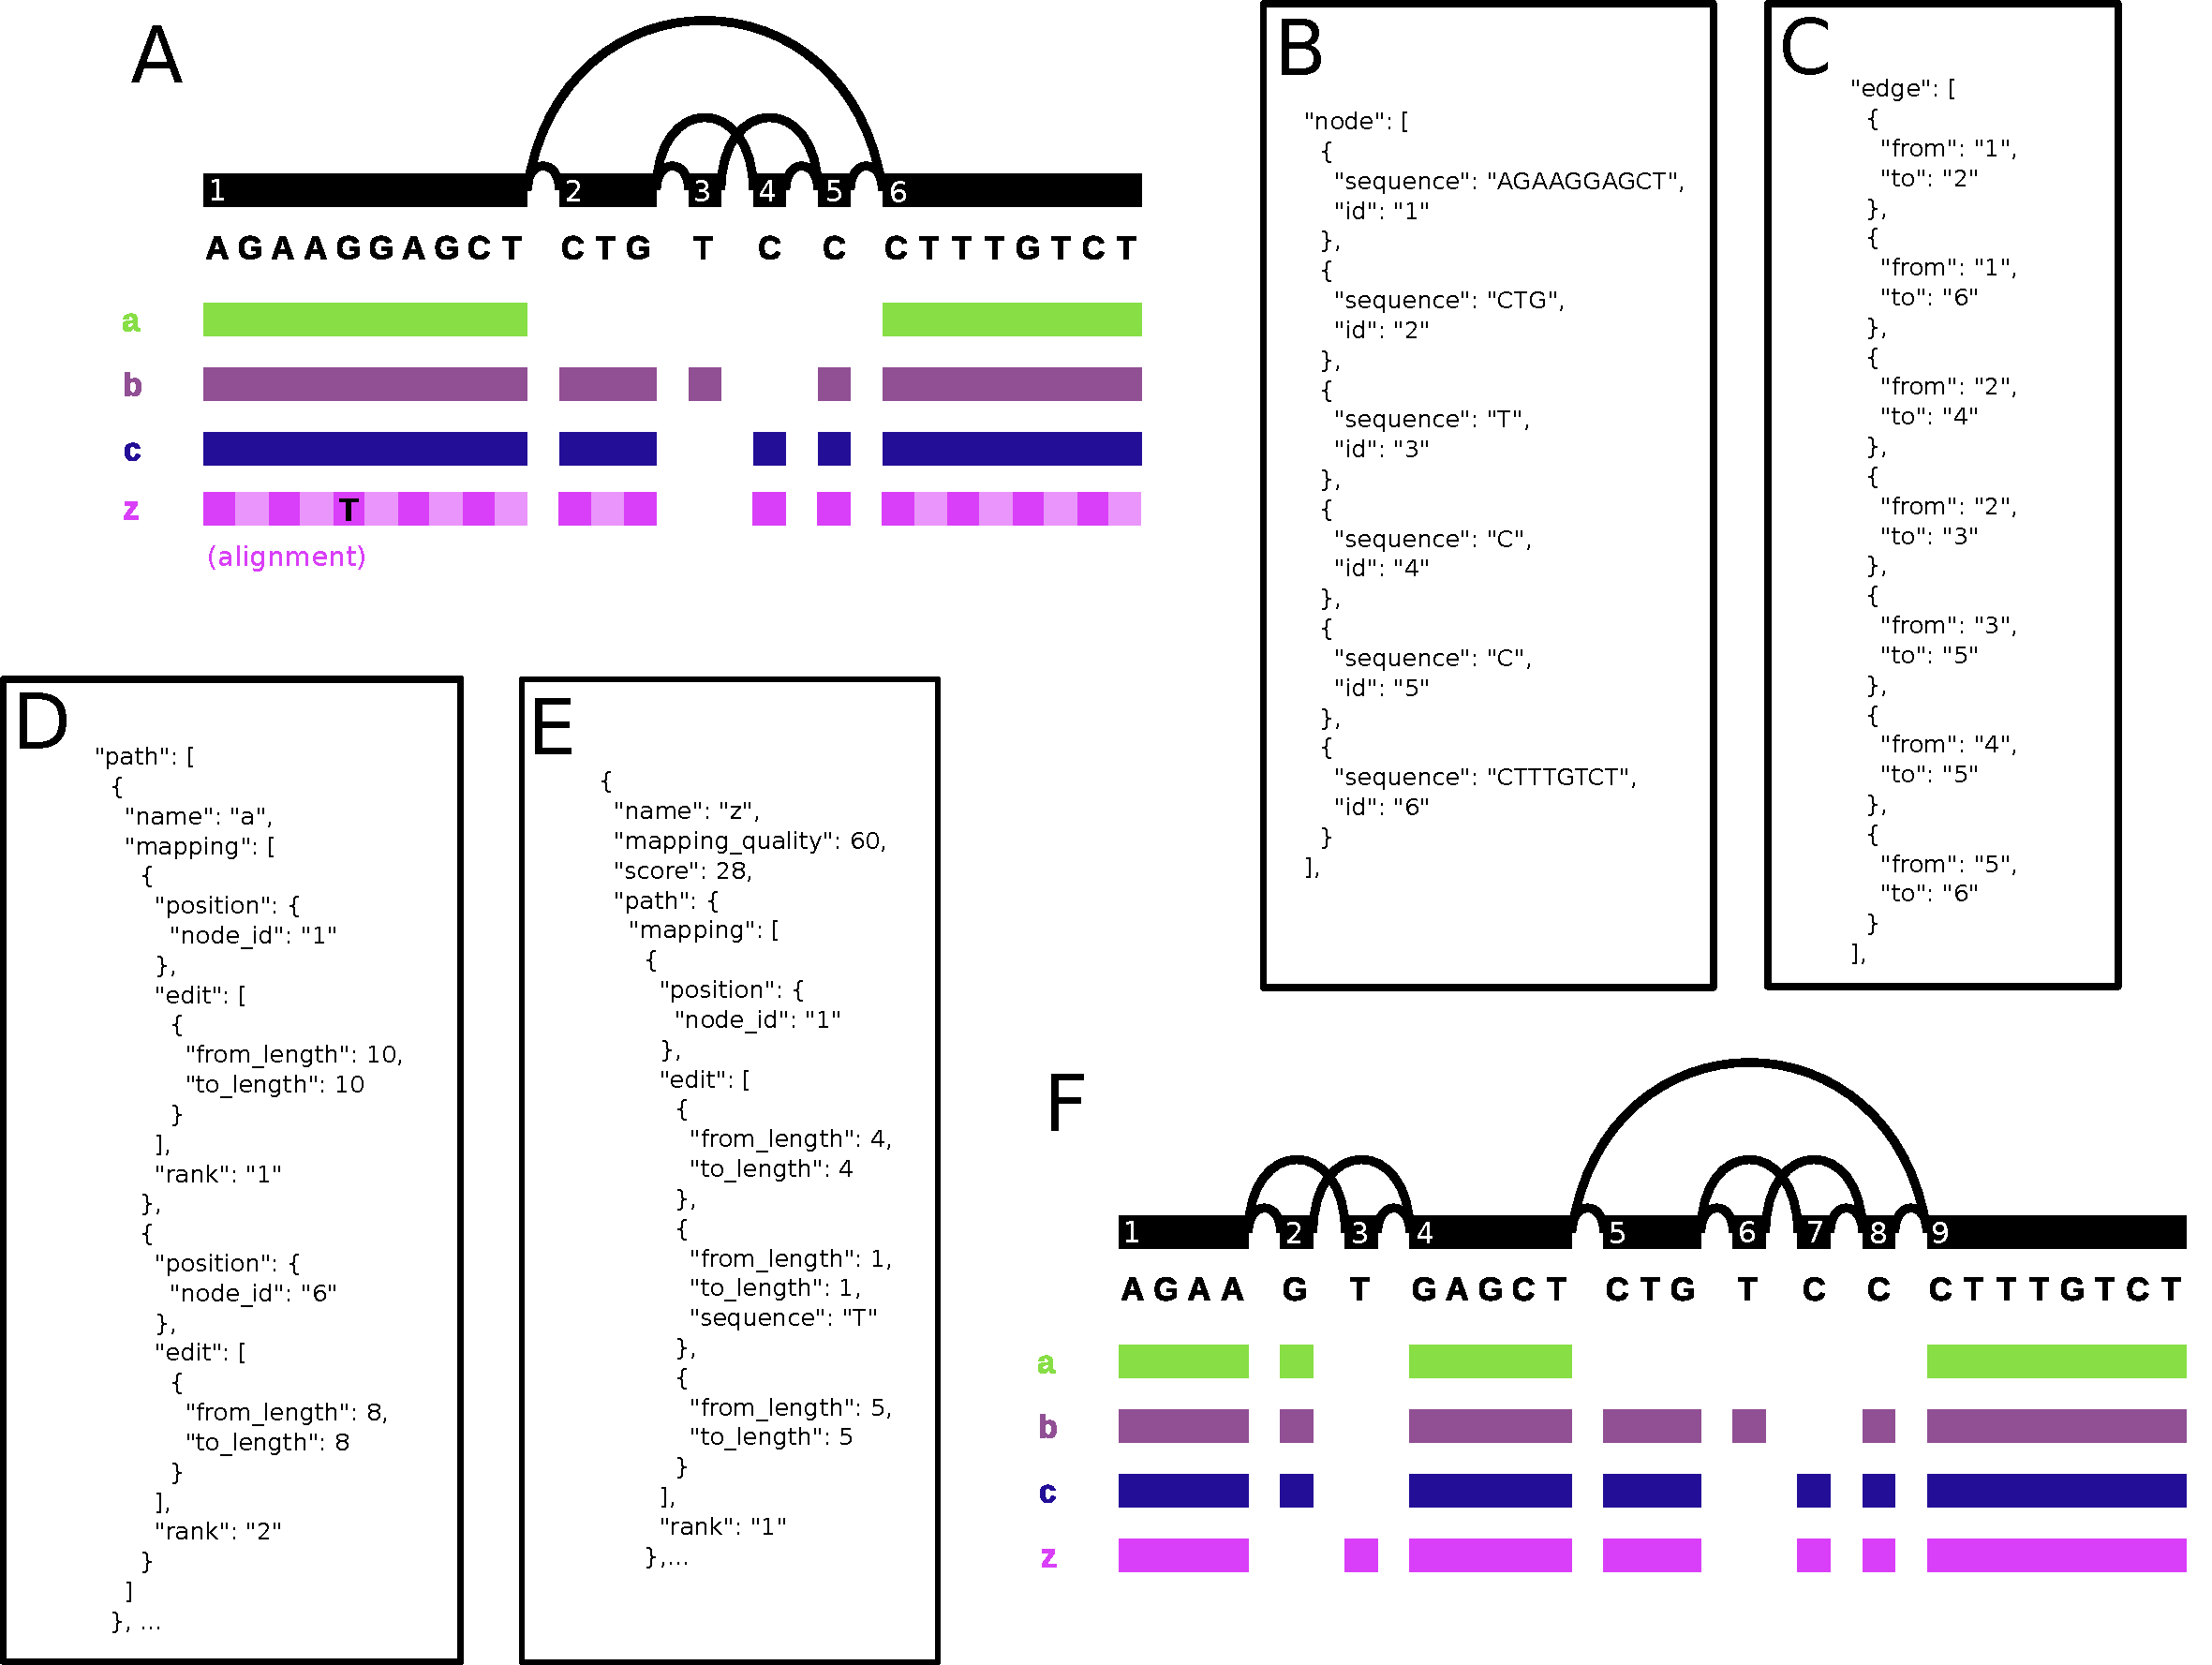
\includegraphics[width=\textwidth]{Chapter2/Figs/example_vg_construction.pdf}
  \caption[The basic elements of a variation graph]{
    A step in the progressive construction of a variation graph from homologous fragments of four haplotypes in the GRCh38 alternate allele set for the HLA gene DQB1-3119.
    (A) shows the variation graph constructed by progressive alignment of three sequences labeled \emph{a}, \emph{b}, and \emph{c}.
    The graph topology is shown at the top of the panel, with nodes represented by black bars, labeled by their node IDs (white numbers), and with edge connections between nodes shown by arcs above.
    Paths are indicated in the colored bars below, with an identifying name to the left.
    This graph is partially ordered, without cycles, and so the sequences of paths may be enumerated by concatenating the node sequences above the filled portions of each of the path rows.
    A fourth sequence \emph{z} has been aligned to the graph, and is shown in a checkerboard magenta pattern.
    It contains a single SNP relative to the graph, which is shown by the black {\tt T} matching the fifth position of the first node.
    The JSON presented in (B) describes the full node set of the graph in (A), while (C) lists the edges.
    (D) shows the path \emph{a} embedded in the graph in full. Other paths are not shown, but are recorded similarly.
    (E) describes the alignment of \emph{z} against graph (A). Only the beginning of the path of \emph{z} against (A) is given.
    The first mapping in the path describes a SNP between the matching subsequence in \emph{z} and $n_1$.
    Note the second edit in the mapping, which specifically describes the SNP as a replacement of a subsequence in $n_1$ by {\tt T}.
    Graph (F) is the result of the application of the $edit$ operation to graph (A) and alignment \emph{z}.
    The node IDs have been reassigned.
    The inclusion of the SNP increases the node count of the graph by 3.
    Path $[n_1]$ in graph (A) maps to $[n_1,n_2,n_4]$ in (F).
  }
  \label{fig:vg_illustrative_example}
\end{figure}

%\section{An extensible graphical model of many sequences}
\section{A generic graph embedding for genomics}

We define a \emph{variation graph} to be a graph with embedded paths $G = (N, E, P)$ comprising a set of \emph{nodes} $N = n_1 \ldots n_M$, a set of \emph{edges} $E = e_1 \ldots e_L$, and a set of \emph{paths} $P = p_1 \ldots p_Q$, each of which describes the embedding of a sequence into the graph.
By generalizing these paths to support edits against the graph, we provide a mechanism to describe relations between the graph and other sequences.
Augmenting the path with additional information important to sequence analysis allows us to construct an \emph{alignment}.
Collections of pairs of paths covering the space of two graphs describe a graph to graph alignment, or \emph{translation} which can be generated when the graph is edited, to allow for the projection of coordinates and sequences in one graph into the space of the other.
A limited form of this translation is a \emph{genotype}, which maps the implied bubble formed across multiple copies of a homologous locus into the space of the graph.
Collections of genotypes are the primary output of resequencing.
Phasing algorithms extend genotypes into longer phased haplotypes, which we record as paths through the graph.
These data models thus provide a sufficient informational basis for resequencing against variation graphs.

\subsection{The bidirectional sequence graph}

Each node $n_i$ represents a sequence $seq(n_i)$ that is built from an alphabet $\Sigma = \{ {\tt A, C, G, T, N} \}$. Nodes may be traversed in either the forward or reverse direction, with the sequence being reverse-complemented in the reverse direction.
We write $\overline{n_i}$ for the reverse-complement of node $n_i$, so that $seq(n_i) = revcomp(seq(\overline{n_i}))$.
Note that $n_i = \overline{\overline{n}}$. For convenience, we refer to both $n_i$ and $\overline{n_i}$ as ``nodes''.

Edges represent adjacencies between the sequences of the nodes they connect.
Thus, the graph implicitly encodes longer sequences as the concatenation of node sequences along walks through the graph.
Edges can be identified with the ordered pairs of oriented nodes that they link, so we can write $e_{ij} = (n_i,n_j)$.
Edges also can be traversed in either the forward or the reverse direction, with the reverse traversal defined as $\overline{e_{ij}} = (\overline{n_j},\overline{n_i})$.
VGs can contain ordinary cycles (in which $n_i$ is reachable from $n_i$), reversing cycles (in which $n_i$ is reachable from $\overline{n_i}$), and non-cyclic instances of reversal (in which both $n_i$ and $\overline{n_i}$ are reachable from $n_j$).

The bidirectional sequence graph underlying the variation graph model is illustrated in panels A, B, and C of figure \ref{fig:vg_illustrative_example}.

\subsection{Paths with edits}
% TODO fixme this needs an explanation of what's different between paths in the graph and those in alignments
We implement paths as an edit string with respect to the concatenation of node subsequences along a directed walk through the graph.
We do not require the alignment described by the edit string to start at the beginning of the sequence of the initial node, nor to terminate at the end of the sequence of the terminal node.
To allow the path model to support differences from the graph, each path is composed of a series of node mappings $p_i = m_1 \ldots m_{|p_i|}$ which are semantically identical to the alignment format used by standard aligners.
Each mapping $m_i = ( b_i, \Delta_i )$ has a starting position encoded as a node and offset in the graph $b_i = ( n_j, o_i )$ and a series of edits $\Delta_i = \delta_1 \ldots \delta_{|m_i|}$.
Edits $\delta_i = ( f_i, t_i, r_i )$ represent a length $f_i$ in the graph node $n_j$ (a ``from length'' in the reference), a length $t_i$ in the sequence the path encodes (a ``to length'' in the query), and an additional sequence $r_i$ that would replace the sequence at the given position in the reference in order to transform it into the query.
In the case of exact matches, we allow the replacement sequence $r_i$ to be empty.

Alignments are often described in terms of matches, mismatches, and indels.
We encode matches when $f_i = t_i \land r_i = \emptyset$, single mismatches when $f_i = t_i = 1 \land r_i \neq \emptyset$, deletions when $f_i > 0 \land t_i = 0 \land r_i = \emptyset$, and insertions when $f_i = 0 \land t_i > 0 \land r_i \neq \emptyset$.
As paths are described by a series of mappings with independent positions, they can represent all kinds of structural variation relative to the graph.
When mapping positions are always at the start of a node, the edit set for the path contains only matches, and the edges traversed by the path are all present in the graph\footnote{Note that paths may contain disjoint mappings that are not connected by edges in the graph, which allows them to represent structural variations.}, we say that the path is \emph{embedded}.
The paths from which we construct the variation graph are fully embedded, and in practice paths that contain differences occur only in the alignment of new sequences into the graph.

The example variation graph in figure \ref{fig:vg_illustrative_example} panel A contains several paths, while panel D explicitly describes a portion of one of the paths using an equivalent model to the one described here.

\subsection{Alignments}
\label{sec:alignments}

Auxiliary read information is important when analyzing collections of DNA sequencing data sets.
Each read has a name, and an identity related to a particular sequencing experiment.
It may be related to a particular genomic sample or individual.
DNA sequence reads themselves result from a previous set of analyses run on raw observations derived from DNA, perhaps fluorescence or current traces or images.
The process of collapsing this raw information into the sequence read yields a confidence in addition to a base call.
These are recorded in a quality string in FASTQ.
The need to collect this information has resulted in the development of the SAM/BAM sequence alignment format, which provides a standard for linking the called bases (sequence), quality information, read name, features of the alignment against a reference genome and additional optional typed annotations.

I follow this same model in developing an alignment format for read alignments to the graph.
An aligned set of sequences $Q$, $A = a_1 \ldots a_{|Q|}$, represents a sequencing experiment.
Each aligned read connects a sequence, an (optional) quality string, a path through the graph including possible edits, and an optional set of $D_i$ annotations: $a_i = (s_i, q_i, p_i, k_1\ldots k_{D_i})$.
In principle the read sequence can be reconstructed from the path, but retaining the sequence information makes the alignment object lossless with respect to the input FASTQ and provides redundancy which can help in data processing.

Panels A and E of figure \ref{fig:vg_illustrative_example} demonstrate how an alignment to a variation graph can encode putative variation, in this particular case encoding a SNP.

\subsection{Translations}
\label{sec:translation}

A generalization of the alignment is the translation set $\Phi = \phi_1 \ldots \phi_{|\Phi|}$, which relates paths in different graphs to describe the mapping between them.
A translation $\phi = (p_f, p_t)$ defines the projection between two paths which may arise in the context of two graphs $G_f$ and $G_t$.
In this use each $p_f$ corresponds to a path relative to $G_f$ (conventionally the base or reference graph), and each $p_t$ to some path in $G_t$.

If each node and edge and path in both graphs is represented in some graph translation in $\Phi$ then it provides an isomorphic relationship between the graphs.
Provided each $\Phi$ encodes an isomorphism, then we can layer a series of $\Phi_i$ together to provide a coherent coordinate space across any number of updates to a given graph.
Consider a function pattern $translate$, which allows the projection of paths relative to $G_f$ through translations $\Phi$ to yield paths in $G_t$: $translate(p_i, \Phi) \to p_j \in G_t$, and similarly allows the transformation of a base graph into a target graph: $translate(G_f, \Phi) \to G_t$.
If we have a series of $(G_i, \Phi_1) \ldots (G_\rho, \Phi_\rho)$, where $translate(G_i, \Phi_i) \to G_{i+1}$ and thus each $\Phi_i$ describes an isomorphism between $G_i$ and $G_{i+1}$, then we can generate a graph translation $\Phi_\Delta$ providing $translate(G_1, \Phi_\Delta) \to G_\rho$.
We build this graph translation with the function $layer(\Phi_\alpha, \Phi_\beta) \to \Phi_{\alpha \circ \beta}$ by rewriting each path translation $\phi_i \in \Phi_\alpha$ so that its $p_t$ refers to $G_\beta$.
We do so by projecting the $p_t$ through $\Phi_\beta$, and finally adding any $\phi_j \in \Phi_\beta$ for which $p_f = \emptyset$, as these represent insertions of new sequence in $G_\beta$ relative to $G_\alpha$.

\subsection{Genotypes}
\label{sec:genotypes}

As path to path relationships can provide descriptions of allelic diversity, they form the basis for a graph-relative genotype encoding.
To represent the exact genotype of a particular sample with ploidy $\nu$ at a given locus $\iota$ we can simply collect the multiset of alleles $\pi_\iota = ( p_1 \ldots p_\nu)$.
We could alternatively build a probabilistic model $\varpi$ of an unphased genotype by using a set of $\mu$ alleles $\{ p_1 \ldots p_\mu\}$.
To do so, we associate likelihoods $\gamma_\xi$ for each possible genotype $\pi_{\iota_\xi}$ that could be sampled from the alleles such that $\varpi = \gamma_1 \ldots \gamma_{\frac{\mu!}{\nu!(\mu-\nu)!} }$.
In practice, we develop our $\gamma_\xi$ out of quality information from the reads and a sampling model related to $\nu$ \cite{garrison2012haplotype,li2011statistical}.
Existing genotyping models can be applied to drive genotyping using read sets aligned to the graph, and the output of the genotyper is defined fully in the space of the graph.

\subsection{Extending the graph}
\label{sec:extending}

Given an alignment $a_i$, we can edit the graph $G$ so that it includes the alignment and the sequence it represents as an embedded path, $augment(G, a_i) \to (G', \Phi)$, such that $translate(p_i, \Phi) \in G'$.
To update the path space of the graph we project all paths, including that of $a_i$, through the translation implied by the augmentation of the graph with $p_i$.
Any other alignment $a_j$ whose path $p_j$ overlaps $p_i$ would no longer be valid, although it could be projected through the graph translation $\Phi$ as well to express it in the space of the new graph $G'$.
Updating the graph one alignment at a time is inefficient as we need to build and layer a new translation for each alignment.
It is simpler to edit the graph in a single step, taking a collection of alignments and including them in the graph, $edit(G, A) \to (G', \Phi)$.

One way to accomplish this is to first take the set of unique mappings represented in the paths of $A$, $\Omega = \{ m_1 \ldots m_{|\Omega|}\}$, and for each $m_i$ cut $n_i$ at the breakpoints where any new variation would need to be added in, adding new nodes to represent the cut portions.
Then, walking through each alignment we add in unique novel sequences and their linkages to the preexisting nodes or new breakpoints to the graph.
This process will disrupt the identifier space of the nodes and edges of the graph, but it naturally yields a translation that can be used as described in section \ref{sec:translation}.
Both alignments and genotypes are based on paths, so this mechanism can be used to extend the graph based on any sequence level differences observed through alignment or variant calling.

Figure \ref{fig:vg_illustrative_example} provides an example to provide a concrete intuition about the $edit$ function.
Editing the graph in panel A with the alignment of sequence \emph{z} yields the graph in panel F.
The corresponding translation is described in the figure legend.

\section{Variation graph construction}

We will use variation graphs as the core model for a number of essential processes in genome inference.
This model can represent many graphical sequence models used in genomics.
Each one necessitates conversion into the variation graph model.
Here I describe the transformation of a number of graphical models into variation graphs, including MSAs, assembly graphs, and alignment graphs induced from pairwise alignments.
In some cases the conversion is direct, but in others it requires the addition of new labels to our model.
Variation graphs may also be built from first principles, provided a function that aligns a sequence into the graph and the editing operations described in \ref{sec:extending}.

\subsection{Progressive alignment}

If we have a series of $k$ queries $q_1 \ldots q_k$, then we can build a progressive alignment by a series of edit and alignment operations applied to the variation graph.
First, take the empty graph $G_\emptyset$, to which any alignment will yield a path $p_1$ that has no mappings and which encodes the query sequence $q_1$ as a replacement sequence in the path.
We then edit the graph to add the sequence using $edit(G_\emptyset, p_1) \to G_1$.
For each subsequent $q_j$ we obtain the next graph by finding the alignment $align(q_j, G_j) \to p_j$ and editing the graph with it to yield the next graph $edit(G_j, p_j) \to G_{j+1}$ until $j = k$ and we obtain our final graph.
This simple approach is attractive as it allows the variation graphs to be built from whole sequences using only techniques that are native to the variation graph model itself.
However, it is obviously order dependent, with potentially different results if the set of input sequences are presented in different orders.
I later presents results based on this multiple sequence to graph alignment process, {\tt vg msga}.

\subsection{Using variants in VCF format}
%*1.5p 1h*
As discussed in section \ref{sec:seq_dag_vcf}, the VCF format that is popular in resequencing implies a sequence DAG.
We can consider how to build a trivial variation graph using the core operation $edit$.
First, we build a variation graph from the reference genome $Q_\textbf{ref}$ : $G_\textbf{ref}$.
This graph contains one path $p_\textbf{ref}$ : $seq(p_\textbf{ref}) = Q_\textbf{ref}$.
As described in section \ref{sec:genotypes} each locus reported in VCF can be encoded as a set of paths $P_\textbf{vcf} = p_1 \ldots p_V$, each representing a different allele.
We now edit the graph to embed these allele paths, $edit(G_\textbf{ref}, P_\textbf{vcf}) \to G_\textbf{vcf}$.
It is possible to regenerate the VCF file input by walking the positions of $p_\textbf{ref}$ and enumerating the overlapping paths as alleles in VCF format.

For efficiency, we have not implemented VCF to variation graph conversion with specifically this algorithm, but instead build up $G_\textbf{vcf}$ by walking along the reference genome $Q_\textbf{ref}$ and processing each locus sequentially.
This exploits the partially ordered property of the VCF to limit memory requirements.
For regions before, after, and between variant records at reference offsets $i$ and $j$ we add a node $n_\textbf{curr} : seq(n_\textbf{curr}) = substr(Q_\textbf{ref}, i, j)$, linking these by edges to those nodes ending at position $i$ of the reference and adding corresponding mappings for the reference path to $p_\textbf{ref}$.
At simple variant sites we add each of the alleles as a new node $n_{\textbf{var}_i}$, including an edge for each $e_{\textbf{curr} \prec \textbf{var}_i}$.
Here we also handle the reference allele differently in that we append a mapping $m_\textbf{ref} = ((n_\textbf{ref}, 0), \emptyset)$ to $p_\textbf{ref}$.

As long as the VCF records are ordered, this process allows for streaming conversion of the VCF format into a variation graph.
However, VCFs used to represent structural variation often do not describe a fully-ordered series of loci.
For instance, a large deletion may be described in one record, and followed by a number of records describing variation on the reference within the scope of the deletion.
In the graph, this results in the nesting of bubbles, and requires a deviation from a simple streaming algorithm in order to be handled.
Deletions must be recorded and linked into the downstream portion of the graph as it is later generated.

VCFs may also encode phased haplotypes, which, like the reference, have a natural representation in the graph as paths.
Parsing these may require multiple passes over the VCF due to the memory requirements for storing large numbers of haplotypes uncompressed and cross-indexed to allow traversal in RAM.
To prevent $O(H|G_\textbf{vcf}|)$ growth of the required memory to store these, we implement compression strategies on the haplotype set that exploit their repetitiveness.
The VCF format does not impose a semantic requirement that the encoded haplotypes are valid, which introduces some complexity in the implementation of this method.
We must break haplotypes where they are found to be invalid in order to record them in VG format.
For instance, a phased VCF may report more than $\nu$ (expected ploidy) alleles for a given individual, such as when deletion and SNP variants overlap.
We expect these haplotype paths to be embedded in the graph.
Although haplotype sets are equivalent to large collections of paths, we term their components \emph{threads} to indicate that they have a simpler representation than arbitrary paths.

\subsection{From gene models} % (GFF)
\label{sec:construct_from_gff}

A reference-based RNA splicing graph is usually expressed as a set of named intervals in BED or the General Feature Format (GFF).
As with the generic VCF generation algorithm, we can convert the transcripts to alignments $A$ relative to the graph.
Then we can then embed the transcript paths in the graph $edit(G_\textbf{ref}, A) \to G_\textbf{splice}$.
Any transcript in our set is thus encoded by the graph, and can be matched to it directly with alignment.
The resulting structure will also support novel isoforms built with splices from the known set.

\subsection{From multiple sequence alignments}
%*0.5p 0.5h*
A multiple sequence alignment in matrix form has a simple translation into a sequence DAG and thus a VG \cite{lee2002POA}.
Given a set of sequences $Q = q_1 \ldots q_\kappa$ their $\upsilon$-long mutual alignment may be described in a $\kappa \upsilon$ matrix $X$ designed to maximize $\sum_{i=1}^{\upsilon} \sum_{j=1}^{\kappa} \sum_{k=1}^{\kappa} \delta_{X_{ij}X_{ik}}$, where $\delta$ is the Kronecker delta, or some generalization of this.
The alphabet used to encode the matrix is the same as the input sequences with the addition of a special gap character $\Box$ which does not match itself, and gaps thus do not contribute positively to the matrix score.
To build a variation graph $G_\textbf{msa}$ from the MSA we proceed from $i = 1 \to \upsilon$ through $X$.
For each unique character ${\cal B}$ in the query alphabet $\Sigma \setminus \Box$ found in each row $i$, we create a node $n_{\cal B}$ in $G_\textbf{msa}$ and append a mapping to each path $p_i$ for which $n_{\cal B} \in q_i$.
We construct the edges of $G_\textbf{msa}$ by taking the distinct pairs of consecutive node traversals found in the path set $P_\textbf{msa}$ produced after the generation of the nodes in MSA traversal.
Adding add an edge $e_{ij}$ for each pair of nodes $(n_i, n_j)$ consecutively traversed in $P_\textbf{msa}$ ensures that our sequences are present as walks through the graph.
We can optionally compact series of nodes (which represent single characters) where no furcations occur to obtain a simpler graph.

Instead of a matrix, we can formulate the multiple alignment as an alignment graph (described in section \ref{sec:genome_alignment_graphs}).
By making this graph bidirectional, and thus equivalent in information content with the Enredo graph, it becomes equivalent to a variation graph.
Aligners that produce data formats of this type, such as Cactus \cite{Paten:2011fva}, can thus be used to produce VGs, so long as the relationship between the input sequences and the graph is recorded and can be converted into a path description.
In section \ref{sec:yeast_cactus} I discuss the use of this method to build a pangenomic reference system for a diverse set of yeast strains.

\subsection{From overlap assembly and de Bruijn graphs}
%*2p 1.5h*

Overlap-based sequence graphs used in assembly, described in sections \ref{sec:overlap_graphs}, \ref{sec:de_bruijn_graphs}, and \ref{sec:string_graphs}, are nearly identical to variation graphs.
The critical difference between these models and the variation graph is that they attach a label to each edge (or node) describing the alignment between the pair of nodes (or edges) which they connect.
Variation graphs do not support such a feature in their basic definition, as it is unimportant for any use besides temporarily representing overlap graphs.
We call the process of transferring sequence information from the edges to the nodes \emph{bluntification}.

We start by assigning the sequence of each node to be the sequence of the corresponding read.
If we shorten the sequence of a node to reduce an overlap between a pair of nodes, it will render other overlaps on the same nodes incorrect.
Thus, it is essential that the bluntification algorithm work by the reduction of sets of overlaps on edges which are transitively closed by connection to the same ends of each node, $net(e_{ij}) \to { \forall e_{i*} \in G } \cup { \forall e_{*j} \in G }$, considering both strands of the graph when doing so.
For each net we apply a function $pinch(net(e_{ij})) \to G_{\textbf{pinch}_{ij}}$, which reduces the overlaps between the nodes in the net into a blunt-edged variation graph.
We then link $G_{\textbf{pinch}_{ij}}$ back into the rest of the graph by connecting with the inbound links to each node involved in the net.

In a de Bruijn graph or string graph as generated by SGA or Fermi2, overlaps are exact matches and so are defined given only a length.
This simplifies the implementation of $pinch$, as no further computation is required to correctly determine the mutual alignment of overlapping sequences.
In contrast, overlaps in a generic string or overlap graph are correctly defined as alignments.
Resolving a single pairwise alignment into structures in the graph is trivial, but it becomes considerably more complex when many sequences map into a transitively closed set of overlaps.
These nets can then be resolved into an alignment graph by an algorithm similar to that given in section \ref{sec:from_pairwise_alignments}, but in practice, {\tt vg} implements bluntification using a pinch graph library developed for whole genome alignment \cite{Paten:2011fva}.

\subsection{From pairwise alignments}
\label{sec:from_pairwise_alignments}

A set of pairwise alignments imply a variation graph, however I know of no contained method that will generate the variation graph or lossless string graph from these alignments.
To explore this, I developed an algorithm to do so that operates in external memory, which I here present in detail.
It operates by conversion of the alignment set into an alignment graph and the subsequent use of this graph in the elaboration of the variation graph including paths representing the input sequences.
The resulting graph is a lossless representation of the input and the alignments between them.
To distinguish the approach from string graphs, which imply error correction, I call this variation graph induction model the \emph{squish graph}.

% seqwish algoritm
{\tt seqwish}\footnote{\url{https://github.com/ekg/seqwish}} implements a lossless conversion from pairwise alignments between sequences to a variation graph encoding the sequences and their alignments.
As input, we typically take all-versus-all alignments, but the exact structure of the alignment set may be defined in an application specific way.
{\tt seqwish} uses a series of disk-backed sorts and passes over the alignment and sequence inputs to allow the graph to be constructed in low memory relative to the size of the input sequence set.
Memory usage during construction and traversal is limited by the use of sorted disk-backed arrays and succinct rank/select dictionaries to record a queryable version of the graph.

%## squish graph induction algorithm

As input, we have $Q$, which is a concatenation of the sequences from which we will build the graph.
We build a compressed suffix array (CSA) mapping sequence names to offsets in $Q$, and also the inverse using a rank/select dictionary on a bitvector marking the starts of sequences in $Q$.
This allows us to map between positions in the sequences of $Q$, which is the format in which alignment algorithms typically express alignments, and positions in $Q$ itself, which is the coordinate space we will use as a basis for the generation of our graph.
We encode the set of input pairwise alignments between sequences in $Q$ as object $A$.
Although these alignments tend to be represented using oriented interval pairs in $Q$, for simplicity and robustness to graph complexity, we describe $A$ as a set of pairs of bidirectional positions (sequence offsets and strands) $[1 \ldots |Q_1 \ldots Q_{|Q|}|]$ , such that $A = \{ (b_{q}, b_{r}), \ldots \}$.
We sort $A$ by the first member ($b_{q}$) of each pair, ensuring that the entries in $A$ are ordered according to their order in $Q$.

To query the induced graph we build a rank/select dictionary allowing efficient traversal of $A$, based on a bit vector $A_{bv}$ of the same length as $A$ such that we record a 1 at those positions which correspond to the first instance of a given $b_{q}$ and record a 0 in $A_{bv}$ otherwise. 
We record which $b_{q}$ we have processed in the bitvector $Q_{seen}$ which is of the same length as $Q$.
This allows us to avoid a quadratic penalty in the order of the size of the transitive closures in $Q$ generated by pairs in $A$.

Now we inductively derive the graph implied by the alignments.
For each base $b_{q}$ in $Q$ not already marked in $Q_{seen}$, we find its transitive closure $c_{q} := \{b_{q}, b_{r_{1}}, \ldots \}$ by traversing aligned base pairs recorded in $A$.
We write the character of the base $b_{q}$ to an entry $s_i$ in a vector $S$, then for each $b_{c}$ in $c_{q}$ we record a pair $(s_{i}, b_{c})$ into $N$ and its reverse, $(b_{c}, s_{i})$ into $P$.
We mark $Q_{seen}$ for each base in each emitted cluster, so that we will not consider these bases in subsequent transitive closures.
By sorting $N$ and $P$ by their first entries, we can build rank/select dictionaries on them akin to that we built on $A$ that allow random access by graph base (as given in $S$) or input base (as given in $Q$).

To fully induce the variation graph we need to establish the links between bases in $S$ that would be required for us to find any sequence in the input as a walk through the graph.
We do so by rewriting $Q$ (in both the forward and reverse orientation) in terms of pairs of bases in $S$, then sorting the resulting pairs by their first element, which yields $L = [(b_{a}, b_{b}), \ldots ]$.
These pairs record the links and their frequencies, which we can emit or filter (such as by frequency) as needed in particular applications.
In typical use we take the graph to be given by the unique elements of $L$.

Our data model encodes the graph using single-base nodes, but often downstream use requires identifying nodes and thus we benefit from compressing the unitigs of the graph into single nodes, which reduces memory used by identifiers in analysis.
We can compress the node space of the graph by traversing $S$, and for each base querying the inbound links.
Maintaining a bitvector $S_{id}$ of length equal to $S$ we mark each base at which we see any link other than one from or to the previous base on the forward or reverse strand, or at bases where we have no incoming links.
By building a rank/select dictionary on $S_{id}$ we can assign a smaller set of node ids to the sequence space of the graph.

Given the id space encoded by $S_{id}$ we can materialize the graph in a variety of interchange formats, or provide id-based interfaces to the indexed squish graph.
To generate graphs in {\tt vg} or GFA format, we want to decompose the graph into its nodes ($S$), edges ($L$) and paths ($P$).
The nodes are given by $S$ and $S_{id}$, and similarly we project $L$ and $P$ through $S_{id}$ to obtain a compressed variation graph.


\section{Data interchange}
%*0.5p 0.5h*

In {\tt vg}, a schema language, Google Protocol Buffers (Protobuf), is used to define a compact description of data structures sufficient for the representation of all the required components.
One cause of this pattern was my involvement in the GA4GH-DWG at the beginning of my thesis, which was then seeking a coherent way of describing graph genomes\footnote{\url{https://github.com/ga4gh/ga4gh-schemas}} to support pangenomic resequencing and related information exchange across the internet.
I implemented the schema for {\tt vg} in the popular Protobuf schema language.
This provided a core API on which to build {\tt vg}.
It also implied a set of streaming data formats, which I implemented as a template library capable of serializing any stream of Protobuf objects.
Due to the reliance on Protobuf, the only code needed to implement reading and writing of these formats is {\tt vg} schema and the stream library\footnote{At the time of writing the schema, \url{https://github.com/vgteam/vg/blob/master/src/vg.proto} and stream parsing library \url{https://github.com/vgteam/vg/blob/master/src/stream.hpp} total around 1000 lines of code, and are sufficient to link any C++ program into the {\tt vg} ecosystem.}.
This greatly simplified the process of developing libraries for working with the variation graph data models.
Although in practice the Protobuf data structures are slower to parse than handmade C-struct serializations like BAM, the amount of effort required to begin writing efficient and structured binary data formats was considerably less with the schema based approach.
Most importantly, the schema based definition of the core data types in {\tt vg} helped new developers and researchers using the system quickly appreciate the basic concepts.

Several data formats are important to {\tt vg}.
In {\tt .vg} format, the graph itself is serialized in non-overlapping chunks, where each edge $e_{ij}$ is stored once in the chunk $G_\textbf{chunk} : n_i \in G_\textbf{chunk}$.
Path mappings must have a rank that identifies their position in the path in order to be subdivided in this way.
This allows them to be read in and rebuilt even if they have been serialized out of order.
A series of alignment objects is a sensible output of the mapping algorithm {\tt vg map}.
The file format produced by writing out a series of Protobuf alignment object serializations using the {\tt stream.hpp} library is called GAM, for Graphical Alignment/Map, in analogy to SAM (Sequence Alignment/Map format).

These data models have various other equivalent serializations.
The GFA format can be used to directly encode VGs.
However, GFA lacks a representation of an alignment with the semantics required by {\tt vg}.
VGs that are partially ordered can be deconstructed into VCF files.
As paths in variation graphs can be used to represent any kind of existing annotations, data providers who represent annotations across many genomes (such as ENSEMBL Genomes) can build their annotation sets which were previously spread across many genomes into a single one embedded in a VG.
To enable this several collaborators\footnote{Jerven Bolleman and Toshiaki Katayama among others.} have developed a Resource Description Framework (RDF) compatible version of the core VG model.

\section{Index structures}
\label{sec:index_structures}

As described in section \ref{sec:sequence_alignment}, the large collections of read data produced by current sequencing methods require efficient read alignment to support downstream analysis.
Typically, these methods develop indexes of their reference genome, using $k$-mer hash tables or FM-index/CSA based data structures that support efficient arbitrary-length exact matching.
These indexes remain static during the resequencing analysis, and can thus be designed to be very compact and to support efficient queries.

When the genome is just a linear string, distances between locations may be computed trivially, and subsets of the sequence are simply substring operations on the vector representing the genome, so no additional structure beyond a full text index is required to seed the alignment of reads to the genome.
However, this situation changes in graphs, where the computation of distances is more complex and particular topologies of the graph must be recorded and reproduced.
Graph distances may be estimated using an approximate sort and the paths embedded in the graph.
However, to do so requires efficient indexes of the path structure in the graph.
Furthermore, loading the entire graph into memory in a na\"{i}ve manner can be very expensive, and effort is required to minimize the runtime costs to enable resequencing even on lower-memory commodity compute servers.

\subsection{Dynamic in-memory graph model}

Serialized in {\tt .vg} or compressed GFA format, the graph of the 1000GP is not much larger than the uncompressed human reference genome.
However, the performance-oriented implementation of the dynamic variation graph which I developed at the beginning of my studies can use a hundred times this much memory when the entire graph is loaded into RAM.
In this scheme implemented in {\tt vg}, indexes on the node identifier space of the graph allow for fast traversal and query of nodes by identity and neighborhood, as well as insertion or deletion of nodes and edges and associated editing of paths.
Various inefficiencies are accepted, such as on the hash table occupancies used to build these indexes, in the pursuit of higher performance during dynamic modification of the graph.
I now believe that it should be easy to provide a dynamic VG in low memory by using a succinct encoding, but I have not yet completed any work on this issue.
Operating on graphs of hundreds of millions of nodes with annotations like paths remains a difficult problem.
In most cases the graph can be subdivided (as with map/reduce processing patterns \cite{dean2008mapreduce} which underpin most industrial operation on large graphs \cite{cohen2009graph}).
This is particularly easy to implement for sequence DAG VGs, allowing for us to work on graphs of arbitrary sizes if they are approximately linear.

\subsection{Graph topology index}
\label{sec:graph_topology_index}
%*2p 3h*

The graph is unlikely to be changed during many kinds of analysis, and so we have the opportunity to compress it into static data structures that provide efficient access to important aspects of the graph with low memory overhead.
Specifically, we care about the node and edge structure of the graph and queries that allow us to extract and seek to positions in embedded paths.
We would like to be able to query a part of the graph corresponding to a particular region of a chromosome in a reference path embedded in the graph.
Similarly, if we find an exact match on the graph using GCSA2, we would like to load that region of the graph into memory for efficient local alignment.

We implement a succinct representation of variation graphs in the XG\footnote{``X'' implies compression and ``G'' refers to the graph that is compressed.} library, using data structures from the C++ toolkit \href{https://github.com/simongog/sdsl-lite}{SDSL-lite} \cite{gbmp2014sea}.
Node labels and node ids are stored in a collection of succinct vectors, augmented by rank/select dictionaries that allow the lookup of node sequences and node ids.
An internal node rank is given for each node, and we map from and to this internal coordinate system using a compressed integer vector of the same order as the node id range of the graph we have indexed.
To allow efficient exploration of the graph, we store each node's edge context in a structured manner in an integer vector, into which we can jump via a rank/select dictionary keyed by node rank in the graph.
Efficient traversal of the graph's topology via this structure is enabled by storing edges as relative offsets to the nodes to which they connect, which obviates the need for secondary lookups and reduces the cost of traversal.
Paths provided to XG are used to induce alternative coordinate systems over the graph. 
We store them using a collection of integer vectors and rank/select dictionaries that allow for efficient queries of the paths at or near a given graph position, as well as queries that give us the graph context near a given path position.

An XG index of $G = (N, E, P)$ is composed primarily of the backing graph vector $G_\textbf{iv} = g_1 \ldots g_{|N|}$, with each $g_i$ recording the edge context for node $n_i$ in the graph: $g_i = ( \eta_i, \Xi_i)$, a sequence vector $S_\textbf{iv}$ recording the sequences labels of the nodes in a bitcompressed form, and a path membership mapping $N_\textbf{path}$.
Each $p_i \in P$ is encoded with a set of structures that allow random access to the graph by path position, which is important for the use of paths as reference coordinate systems in the graph.
A visual sketch of this model is provided in figure \ref{fig:xg_index}.

\begin{figure}[htbp!]
  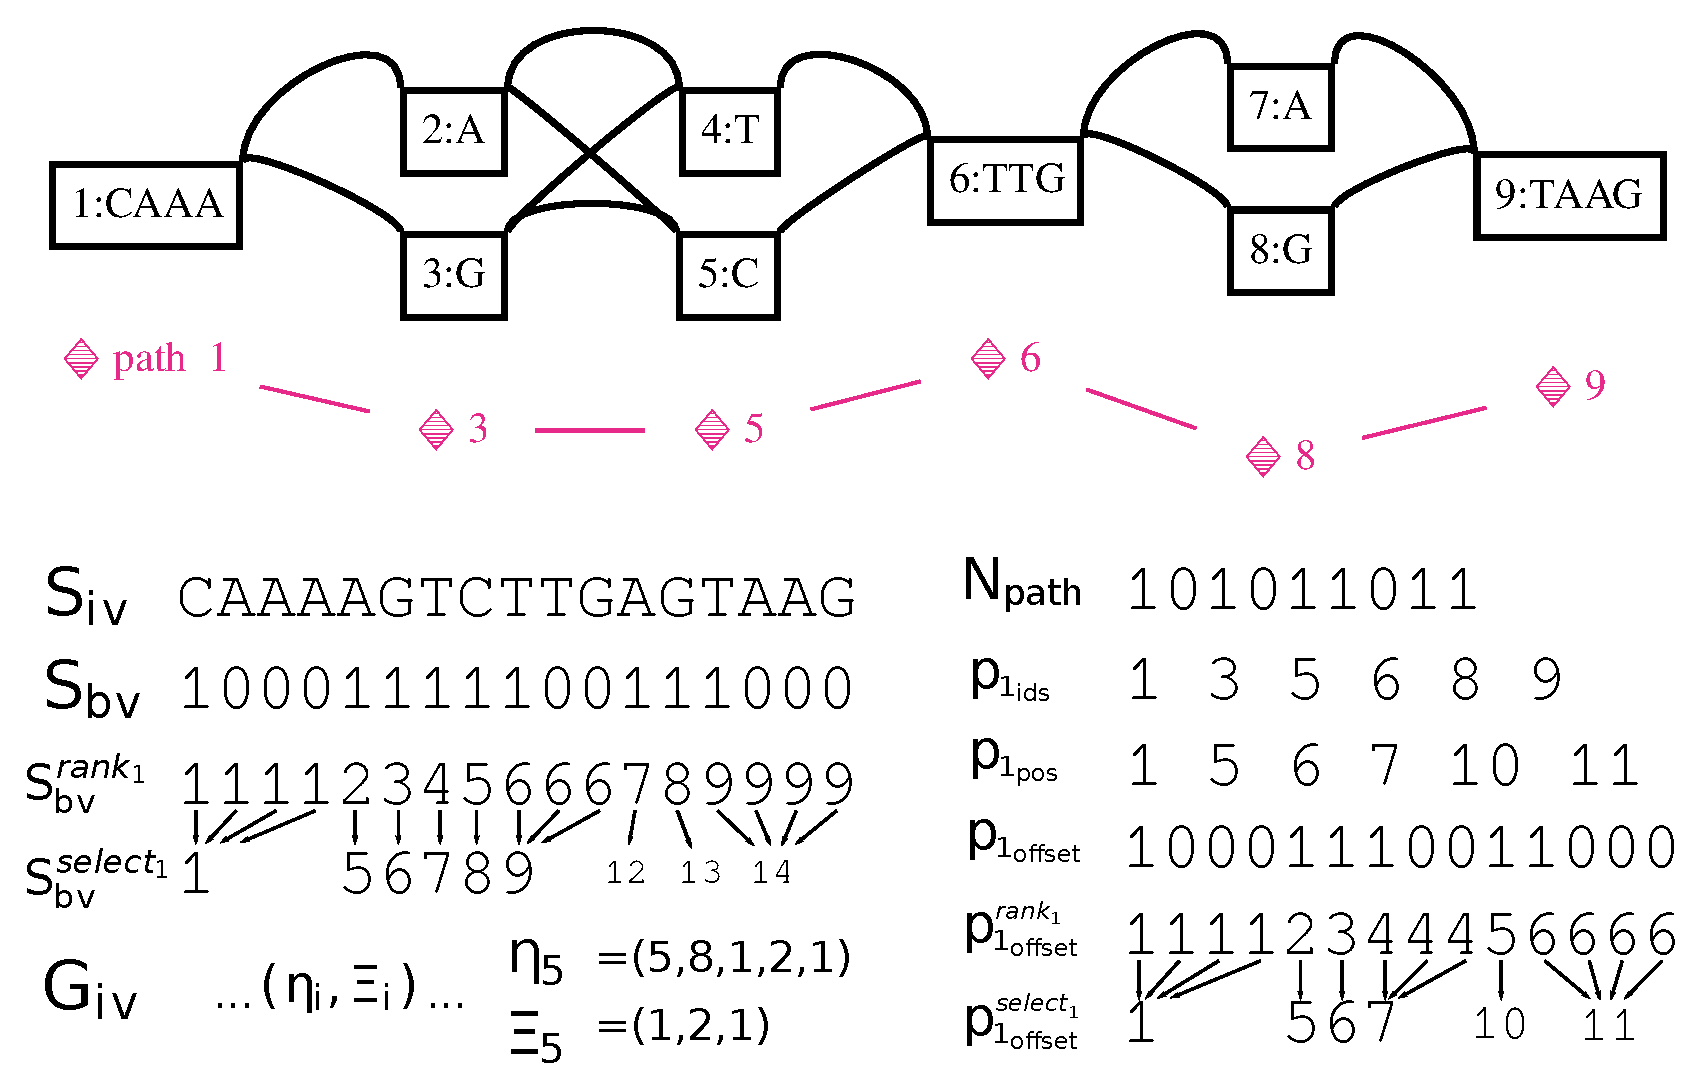
\includegraphics[width=\textwidth]{Chapter2/Figs/xg_index_sketch_nice.pdf}
  \caption[A sketch of the XG index]{
    A visual presentation of the key elements of the XG index for the given graph.
  }
  \label{fig:xg_index}
\end{figure}

To enable better compression, the node sequence space is recorded as a concatenation of node labels $S_\textbf{iv} = seq(n_i) \ldots seq(n_{|N|})$, in which each node has an offset in this sequence space defined by $seq_\textbf{offset}(n_i)$.
In bitvector $S_\textbf{bv} : |S_\textbf{bv}| = |S_\textbf{iv}|$ we set 1 at each first character in a node label, and 0 otherwise: $S_\textbf{bv}[i] = 1 \iff \exists j : seq_\textbf{offset}(n_j) = i \lor 0$.
Random access by node rank $i$ is provided by function $S_\textbf{bv}^{select_1}$, allowing us to find the sequence given a node rank in $G_\textbf{iv}$.

Each $\eta_i$ records node contextual information, including an external id, its offset in the sequence vector, and the degree of $n_i$ in terms of inbound and outbound nodes: $\eta_i = \left[ id(i), seq_\textbf{offset}(n_i), |seq(n_i)|, in(n_i), out(n_i) \right]$.
The use of an external identifier allows the index to work on subsets of larger graphs, and the information about node degree allows us to parse the edge records and efficiently traverse $G_\textbf{iv}$.

The edge context $\Xi_i$ enumerates the set of edges that connect to this node in a structured way that allows for oriented traversals across the two strands of the graph.
To enable fast traversal we rewrite the edges in terms of relative positions in the encoded $G_\textbf{iv}$ vector, which is stored as a bitcompressed integer vector using SDSL-lite's template primitives.
Each node record is stored contiguously.
We delimit the records by a secondary bitvector $G_\textbf{bv}$, for which we build supports for functions $G_\textbf{bv}^{rank_1}$ and $G_\textbf{bv}^{select_1}$, which allow random access of $G_\textbf{iv}$ by node $id$.
Previous designs decomposed the graph structure into a set of parallel vectors, but this required multiple select queries during traversal and provided poor cache locality and performance.

Node to path membership is recorded in an integer vector $N_\textbf{path}$, which contains a contiguous record of path ids that cross each node.
Random access to $N_\textbf{path}$ is provided by a rank/select dictionary built on a bitvector delimiting the various node path membership lists.
Nodes with no path membership are marked in $N_\textbf{path}$ with a 0.

Each path is represented in a set of succinct data structures that let us walk the path by starting at a particular node, query the path position of a given node, or find the node at a particular path position.
We store the path $p_i = m_1 \ldots m_{|p_i|}$ by decomposing its mappings into the nodes (id and orientation) it traverses $p_{i_\textbf{ids}} = id(n_j) \forall n_j \in p_i$ and $p_{i_\textbf{dir}}$ such that $p_{i_\textbf{dir}}[j] = 0 \iff m_j = (n_j, \ldots) \lor 1 \iff m_j = (\overline{n_j}, \ldots)$.
To allow rank and select queries on the node ids, we can store $p_{i_\textbf{ids}}$ in a wavelet tree, although in practice performance is greatly improved by also recording a minimum node id, which decreases the alphabet size and thus memory and runtime costs of the wavelet tree.
So that we may transform nodes to path positions, we use an integer vector to store a path position for each node traversal in the path, $p_{i_\textbf{pos}}$.
To go from path offset to node, we build a bitvector that marks the beginning of each node traversal in the path in a manner similar to that used to mark the sequence beginning of each node in $S_\textbf{iv}$, such that $p_{i_\textbf{offset}}$ is a bitvector of length $\sum_{j=1}^{|p_i|} |seq(p_i[j])|$ where we have marked 1 for each node start in the path, $p_{i_\textbf{offset}}[j] = \left( 1 \iff \exists n_k \in p : j = \sum_{m=1}^{k} |seq(p_i[m])| \right) \lor 0$.
By implementing $p_{i_\textbf{offset}}^{rank_1}$ we can find the node at a given path position $\mathcal{Q}$ by $p_{i_\textbf{offset}}^{rank_1}(\mathcal{Q}) \to j : \left( \sum_{k=1}^{j} |seq(p_i[k])| \leq \mathcal{Q} \land \sum_{k=1}^{j+1} |seq(p_i[k])| > \mathcal{Q} \right)$.
We can also find the position of the $j$th node in a path as $p_{i_\textbf{offset}}^{select_1}(j)$.
A compressed suffix array (CSA) and rank dictionary $P_\textbf{csa}$ and $P_\textbf{name}^{rank_1}$ map from path name to internal rank of the path in $P$.

A number of compression techniques can be applied to the data models in XG to reduce the size of the overall index without any loss in functionality.
However, many of these compression methods producing compressed bitvectors, integer vectors, and wavelet trees, will result in slower access.
In the context of read alignment, such losses may be undesirable as long as there is sufficient memory to load the entire index into system memory, and so I have tuned the index by choosing compression strategies appropriate for its use on current datasets.

\subsection{Graph sequence indexes}
\label{sec:graph_sequence_indexes}
%*1p 2h*

As I presented in section \ref{sec:sequence_alignment}, sequence alignment is driven by sequence indexes that allow efficient queries of subsequences in a given corpus (for instance a reference genome, or a set of reads).
Two main varieties have proved useful.
In $k$-mer indexes, short subsequences of length $k$ are recorded in a hash table or equivalent data structure that allows efficient lookup.
The keys in this table are the $k$-mers, while the values are typically a list of strand-oriented positions in the target set of sequences.
BWT-based indexes emulate the suffix tree of their input text in small space, and allow $O(l)$ time queries for sequences of length $l$, irrespective of the size of the target corpus.
Implementations of the popular FM-index \cite{fmindex2000,fmindex2005} and the functionally equivalent compressed suffix array (CSA) \cite{grossi2005compressed} compress the BWT using encodings that allow fast decompression or direct operation on the compressed data (compressed for example with run-length compression, or that of Raman, Raman, and Rao \cite{raman2002succinct}), and augment the BWT with positional information that allows the index to be used for substring matching.

Indexing the sequence space of variation graphs requires a generalization of the principles behind these indexing techniques.
Junctions allow for the representation of alternative sequences, with an exponential size relative to the number of furcations in the graph.
This introduces problems of representation and scale which have required substantial work to resolve.
In {\tt vg}, I was ultimately to encourage the development of and use a practical implementation of a succinct data structure akin to the CSA, the GCSA2.
This model was developed within the context of {\tt vg}, and is the first sequence index specifically designed to work on variation graphs.
It generalizes concepts and algorithms from the CSA to any kind of bidirectional sequence graph.
Here, I will provide a description of related data structures from which this model draws inspiration, as well as a careful summary of the GCSA2 and the features which make it ideal as the core sequence index to drive a short read to variation graph mapper.
Due to space, I will not fully elaborate this model, as it is not among my contributions.
Readers are encouraged to examine the cited works if they seek a complete description of this and related data structures.

\subsubsection{Graph $k$-mer indexes}

It is straightforward to construct a $k$-mer index of a variation graph.
We simply enumerate the $k$-length walks through the sequence space of the graph.
Problematically, the $k$-mer space of a graph can grow exponentially where variant bubbles cluster within the given length $k$.
To mitigate this issue, we can short-circuit the $k$-mers enumeration when a given number of edges are crossed within $k$ characters.
Another way to mitigate the limitations posed by the exponential number of $k$-mers in the graph is to build the index on disk, rather than using main memory.
In the early stages of the {\tt vg} project, I implemented a $k$-mer based index using a disk-backed system (see section \ref{sec:generic_disk_backed_indexes}).
By sorting the $k$-mers, the index could be efficiently compressed, but still the graph for the human 1000 Genomes Project required over 200GB of memory, and was too slow to use unless cached in main memory.
This index formed the basis for the first prototypes of the {\tt vg} mapper, but is impractical due to its time and memory requirements.

\subsubsection{The FM-index and Compressed Suffix Array (CSA)}
\label{sec:fmidx_csa}

As introduced in section \ref{sec:compressed_full_text_indexes}, compressed full text self indexes like the CSA and equivalent FM-index provide functionality similar to that of the suffix tree (as in Figure \ref{fig:suffix_tree}) but in compressed space.
The functionality of these indexes is the basis for the indexing techniques applied in {\tt vg} to the alignment of reads to variation graphs.
Here, I will first illustrate the construction of a full text index based on the Burrows Wheeler transform (BWT) and suffix array (SA), and show how it can be used to locate occurrences of a pattern in the source text.
This discussion will form the basis for an elaboration of the generalizations that lead to a similar kind of index built over a variation graph.

\begin{figure}[htbp!]
  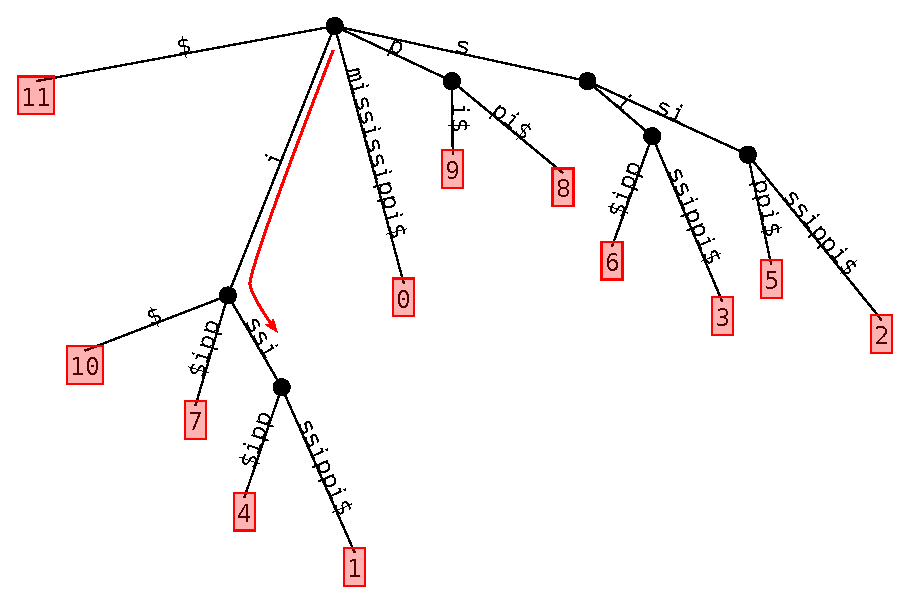
\includegraphics[width=\textwidth]{Chapter2/Figs/mississippi_suffix_tree.pdf}
  \caption[An example of a suffix tree]{
    A suffix tree built from the suffixes of the string {\tt mississippi}.
    Suffixes begin at the root, shown at the top.
    Leaves are labeled by their suffix, which is written in terms of the 0-based starting position of the suffix in the source text.
    A red arrow shows a search for the string ``iss'' on the tree.
    The leaves of the tree below the ultimate point reached by this search give the positions of the matched pattern in the source text, in this case 1 and 4.
    Rendered with \url{https://github.com/mpetri/draw-suffix-tree}.
  }
  \label{fig:suffix_tree}
\end{figure}

To construct the BWT from a given string $T$, we first append a marker character that is outside the alphabet (e.g. {\tt \$}) to the text.
We take all rotations of this string, and lexicographically order them to form a matrix, which is sometimes referred to as the Burrows Wheeler matrix (BWM).
The first column of this matrix is $F$, and lists the characters in the source text in lexicographic order.
We can compactly represent it as a vector of counts $C$ of characters that are lexicographically smaller than a given one, indexed by the characters as encoded in a compact set of integers.
The last column of the BWM is the Burrows Wheeler transform (BWT) of the source text.
The order in which the rotations (or equivalently, suffixes) appear in the sort is the suffix array (SA) of the text.
Assume a function $rank_{BWT}(c, i)$ which returns the number of characters equal to $c$ in the prefix of $BWT[0\ldots i]$.
The function $LF(i) = C[c] + rank_{BWT}(c, i) - 1$ reconstructs the mapping between the same character in the BWT and $F$, thus provides a way to unwind the permutation generated by the sort and reconstruct the source text.
These construction steps are illustrated in Figure \ref{fig:bwt_construction}.

\begin{figure}[htbp!]
  \centering
  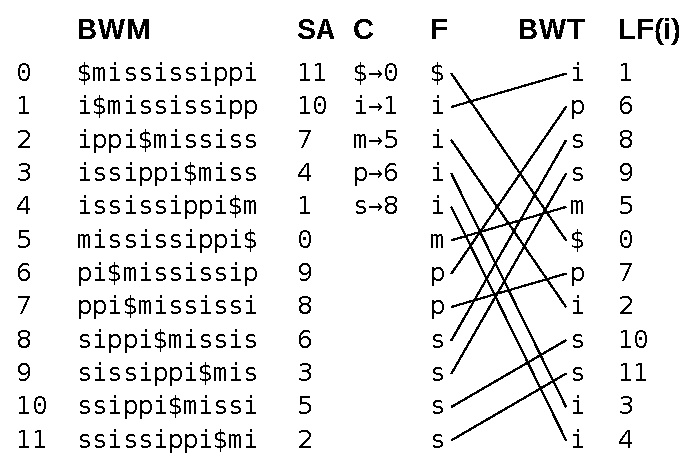
\includegraphics[width=0.65\textwidth]{Chapter2/Figs/mississippi_bwt_construction.pdf}
  \caption[Building the BWT and suffix array]{
    A BWT and suffix array built from the string {\tt mississippi}.
    The Burrows Wheeler Matrix (BWM) shows all rotations of the string (appended with terminal marker {\tt \$}) in lexicographical order.
    $SA$ provides the suffix array, which lists the suffixes relative to the original string in their sorted order in the BWM.
    The first column of the BWM corresponds to vector $F$, which contains a series of runs of single characters in their lexicographic order, and is compactly represented in $C$.
    We find the $BWT$ in the last column of the BWM.
    The function $LF(i)$ is shown for each position in the $BWT$, and lines drawn between $F$ and $BWT$ show the characters in the system that have the same identity in the source text.
    Produced using \url{https://github.com/ekg/drawbwt}.
  }
  \label{fig:bwt_construction}
\end{figure}

We can iteratively apply $LF$ mapping to execute search on the BWT.
Algorithm \ref{alg:bwt_find} defines the function $find(Q)$, which returns the suffix array interval (or lexicographic range) in which suffixes are prefixed by $Q$, should it exist, and an empty interval if $Q$ is not a substring of $T$.
We begin our search by looking at the SA interval prefixed by the last character in our pattern, which is trivially obtained from array $C$.
The body of the loop constitutes one step of backward searching.
Searching works by maintaining the invariant that the prefix of the suffixes in the SA interval defined by $[sp, ep]$ is that given by the set of characters that we have considered in reverse order from the query string $Q$.

\begin{algorithm}
  \caption[BWT find]{
  Backward searching on the BWT
  }
  \label{alg:bwt_find}
  \begin{algorithmic}
    \Function{find}{Q}
    \State $c \gets Q[|Q|-1]$ \Comment{Current character in our search}
    \State $sp \gets C[c]$ \Comment{Beginning of our SA interval}
    \State $ep \gets C[c+1]-1$ \Comment{End of our SA interval}
      \For{$i \in [|Q|-2 \ldots 0]$} \Comment{Step backwards through the string}
        \State $c \gets Q[i]$ \Comment{Update our character}
        \State $sp \gets C[c] + rank_{BWT}(c, sp - 1)$ \Comment{Update $sp$ dependent on $c$}
        \State $ep \gets C[c] + rank_{BWT}(c, ep) - 1$ \Comment{Do the same for $ep$}
        \If{$sp > ep$} 
          \Return{$\emptyset$}  \Comment{We do not find $Q$ in our text}
        \EndIf
      \EndFor \\
      \Return{$[sp, ep]$} \Comment{Return the SA interval prefixed by $Q$}
    \EndFunction
  \end{algorithmic}
\end{algorithm}


\begin{figure}[htbp!]
  \centering
  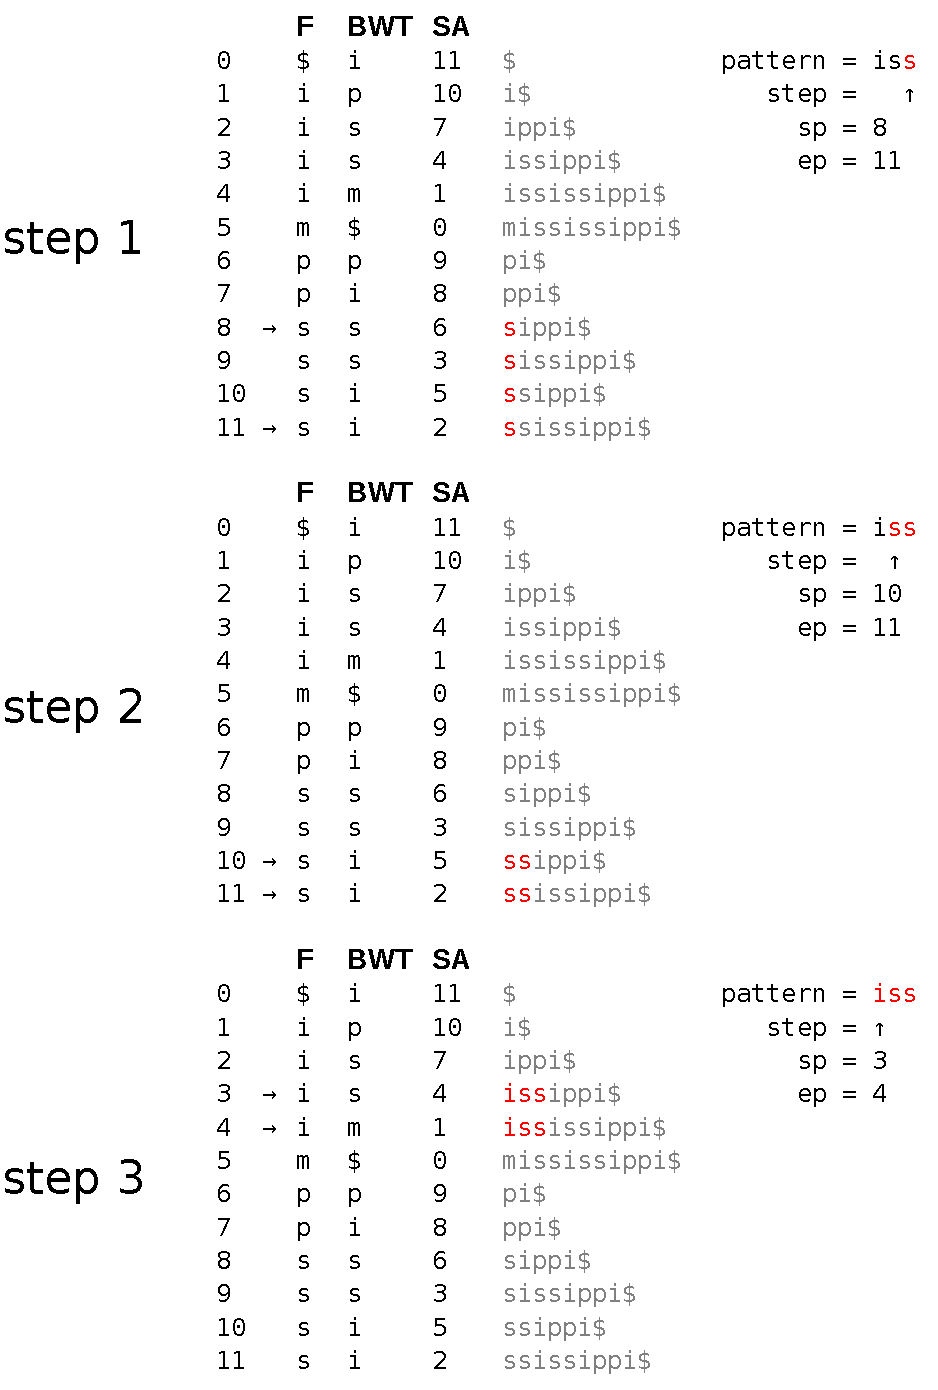
\includegraphics[width=0.65\textwidth]{Chapter2/Figs/mississippi_iss_search.pdf}
  \caption[Backward search in the BWT and suffix array]{
    Using backward search to find all occurrences of {\tt iss} in {\tt mississippi}, using the BWT and suffix array constructed in Figure \ref{fig:bwt_construction}.
    The index structure is shown in each of the three required steps (1$\to$3), which progress from top to bottom.
    At each step, we consider a character, beginning from the end of the string we are searching.
    We apply $LF$ mapping to find the new SA interval corresponding to the backwards extension of our query pattern.
    The subsequence matched up to the current step is shown in red in the sorted suffixes (in gray) represented by $F$, $BWT$, and $SA$.
    We do not store these sorted suffixes, as they are given by the $BWT$ and $SA$.
    Nor do we store $F$, as the $C$ array is sufficient to reconstruct it.
    Rendered with \url{https://github.com/ekg/drawbwt}.
  }
  \label{fig:bwt_search}
\end{figure}

The addition of the longest common prefix (LCP) array on the sorted suffixes allows the CSA to emulate all algorithms on suffix trees \cite{abouelhoda2004replacing}.
This augmented data structure provides a compact encoding of the full suffix tree topology.
In {\tt vg}, an equivalent generalization is used to enable the determination of maximum exact matches between query $P$ and the sequences of a graph.


\subsubsection{BWT-based tree and graph sequence indexes}

In contrast to $k$-mer based indexes, generalizations of the CSA to graphs have required substantial conceptual development to produce.
But, they have yielded compact, efficient data structures that require similar space to their linear counterparts while supporting a wide array of query patterns.

Most generalizations of succinct self indexes from strings to graphs draw on the XBW transform \cite{ferragina2005structuring}, which provides a compressed self index of trees based on a generalization of the FM-index \cite{ferragina2009compressing}.
In the XBW transform (figure \ref{fig:xbw}), rather than considering all suffixes of a linear sequence in the construction of the BWT, we sort all concatenated paths from the root to leaves of each node in the tree and use this as the basis for the BWT in a manner analogous to the use of sorted suffixes for a linear sequence.
To record the topology of the tree and support its navigation relative to the resulting BWT, auxiliary bitvectors record which edges connect to leaf nodes $e$ (or equivalently, an expanded alphabet as originally presented in \cite{ferragina2005structuring}), and which are the last edge among their siblings: ${\cal F}$.
Rank and select queries on these bitvectors allow the generalization of the \emph{LF-mapping} (last-first) permutation and its inverse $\Psi$ to work on the tree.
The lexicographic ranks of the standard versions of these functions are mapped into the appropriate BWT ranges using rank and select queries on ${\cal F}$.


\begin{figure}[htbp!]
  \centering
  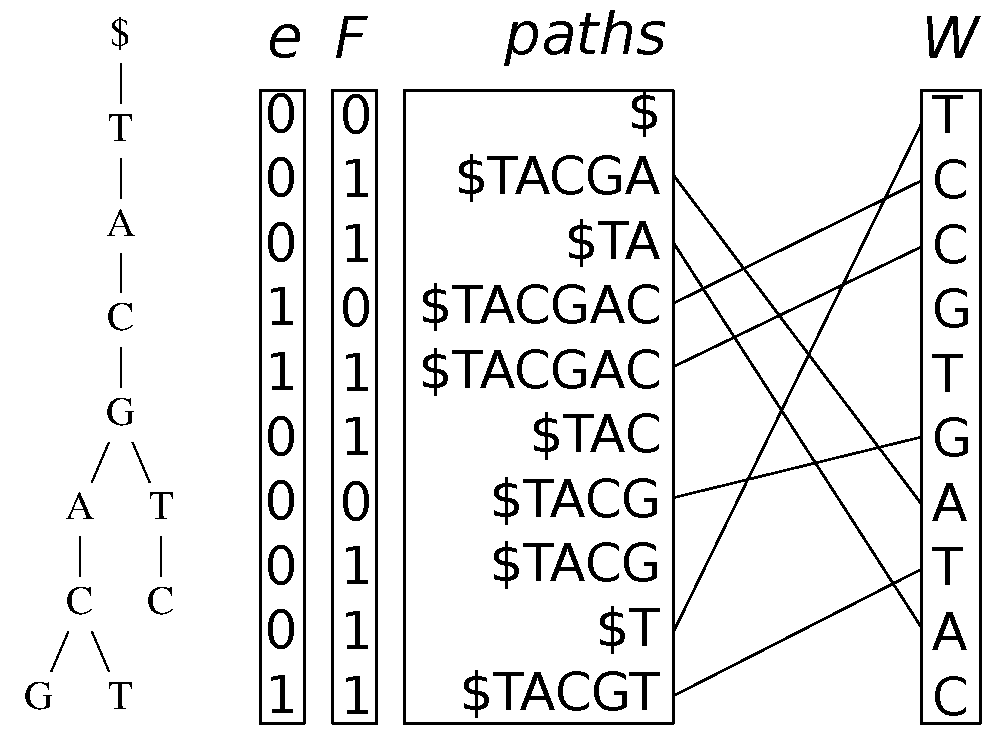
\includegraphics[width=0.6\textwidth]{Chapter2/Figs/xbw_viz.pdf}
  \caption[The XBW transform]{
    The XBW transform and the $LF$ function computed for the given graph.
    Nodes are stored in $W$, while bitvector $e$ marks the leaf nodes (whose LF-mapping is $\emptyset$), and bitvector ${\cal F}$ marks the last nodes in each set of siblings.
    By construction, siblings are sorted together in the set of sorted paths.
    Paths are not stored, but are shown here for clarity.
    Example adapted from a public talk by Alex Bowe, posted at \url{https://pdfs.semanticscholar.org/e42a/daab2806d5c0d715cb812c3a10aa26a2c75a.pdf}.
  }
  \label{fig:xbw}
\end{figure}


Succinct de Bruijn graphs (SDBG) extend the XBW model to support DBGs by recording both in and out degree for each node \cite{bowe2012succinct,muggli2017succinct}.\footnote{See \url{https://alexbowe.com/succinct-debruijn-graphs/} for a high-level overview of Bowe's initial model for succinct DBGs, which explains in detail how the various graph traversal and query operations are implemented.}
In {\tt vg}, we do not use the SDBG model directly, but it is important to describe here as the GCSA2 model draws heavily on its design.

To construct the SDBG (illustrated in figure \ref{fig:sdbg}), we build two sorted lists of tuples representing the edge and $k$-mer space of the DBG $G = (N, E)$.
First, we pad the graph with additional nodes labeled by a character lexicographically lower than the alphabet of the graph, so that each $k$-mer in $G$ is now reachable from a path at least $k-1$ long.
This ensures that we can reconstruct the graph without loss.
In $F$, we record the list of $G$'s edges sorted co-lexicographically by the reverse sequence of their \emph{ending} node and their label.
In $L$, we record the list of $G$'s edges sorted co-lexicographically by the reverse sequence of their \emph{starting} node and their label.
The edge-BWT (EBWT) is the sequence of edge labels as given in $L$.

Navigation of the graph is provided by the mapping between $F$ and $L$ that is based on the relative stability of sorting of edges with the same label in the two lists.
If an edge $e$ is in position $p$ in $L$, and $l(e)$ is a function that gives the character label of edge $e$, then its position in $F$ is given by $|{d : d \in E \land l(d) \prec l(e)}| + rank_{EBWT}(l(e), p) - 1$.
Note that this function corresponds to $LF$ mapping on the BWT.
A similar extension of this idea affords backward search of patterns in node labels in the SDBG.
For full navigation, we must edge topology bitvectors $B_F$, which marks the last edge for each node in $F$, and $B_L$, which does the same for $L$.
We can traverse the graph using these structures.
Given a character $c$ and the co-lexicographic rank of a node, we can use $B_L$ to find the interval in $L$ containing its node's outgoing edges, then find the edge $e$ labeled $c$ in the $EBWT$, and finally use $B_F$ to find the co-lexicographic rank of $e$'s ending node, should it exist.

\begin{figure}[htbp!]
  \centering
  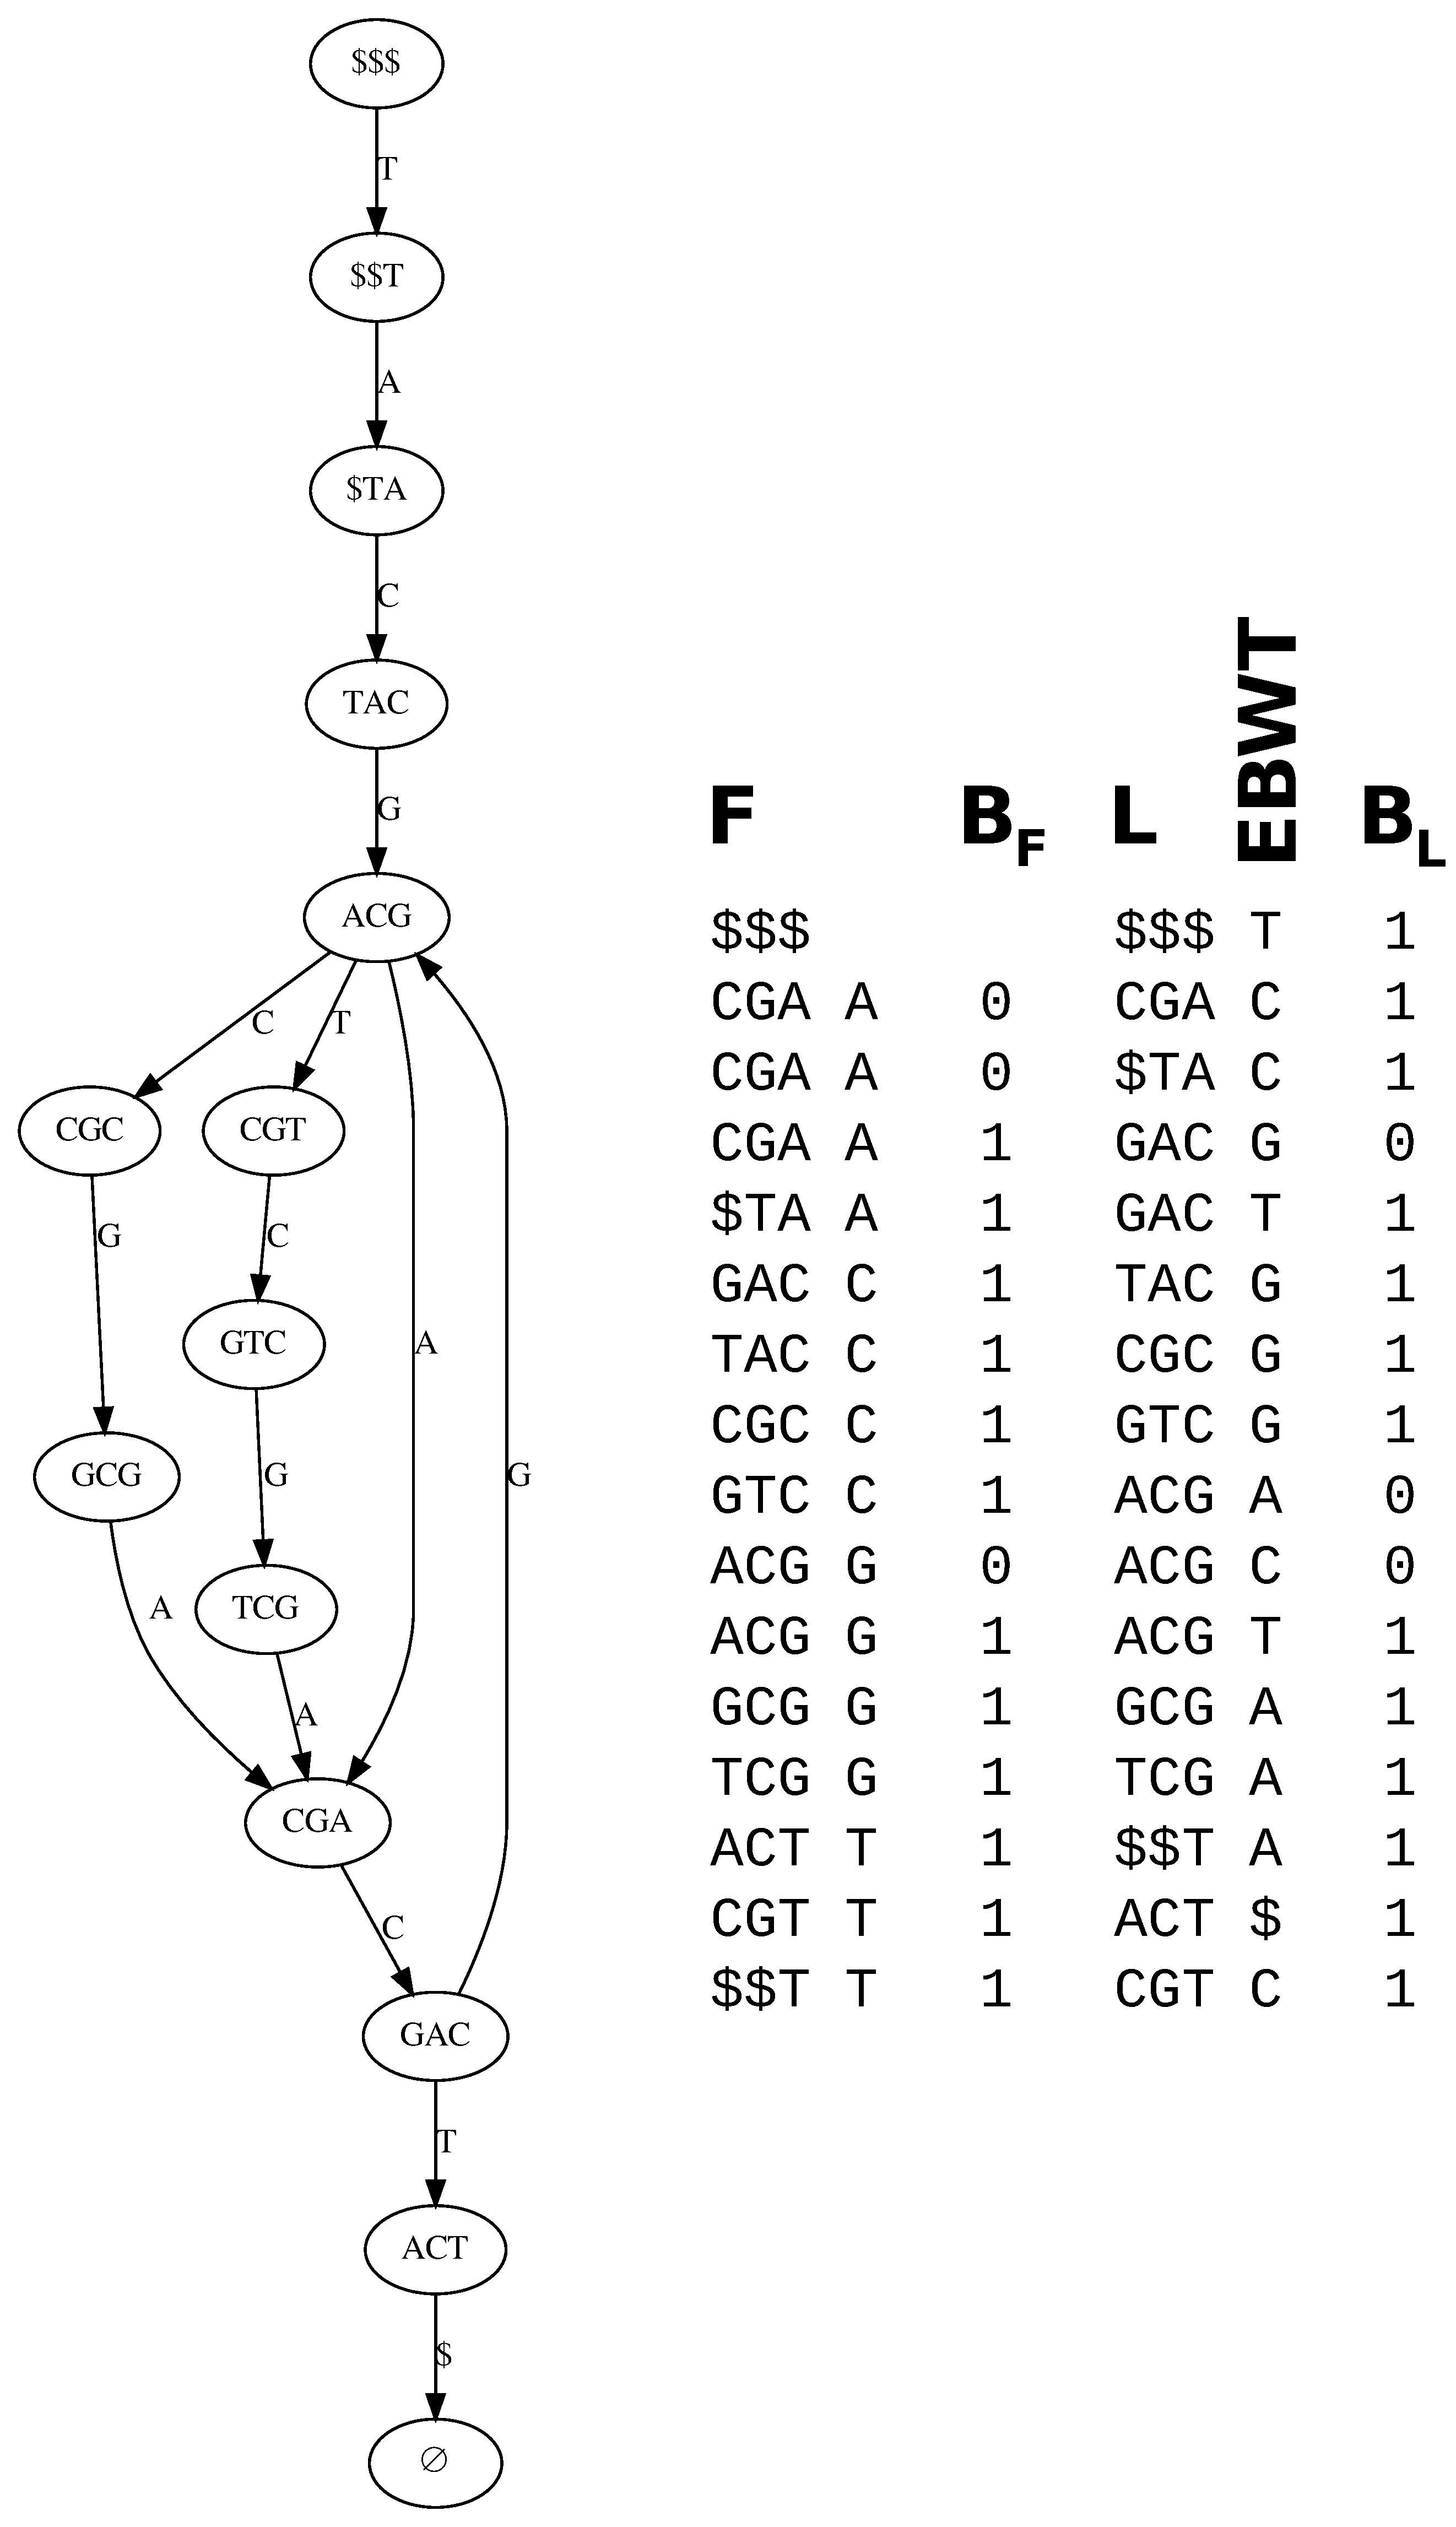
\includegraphics[width=0.65\textwidth]{Chapter2/Figs/sdbg_construction.pdf}
  \caption[Succinct de Bruijn graph construction]{
    On the left, a de Bruijn graph with $k=3$, with edges labeled by the character transition that they imply.
    Right, the construction of the succinct de Bruijn graph for the given graph.
    $F$ indicates the co-lexicographically sorted set of edges keyed by the node that they enter.
    $L$ indicates the co-lexicographically sorted set of edges keyed by the node that they leave.
    $B_{F}$ marks if the edge in $F$ is co-lexicographically the last for its corresponding node, and $B_{L}$ marks the last edge for a given node in $L$.
    The ``edge BWT'' or $EBWT$ is given as the set of edges ordered as in $L$.
    The SDBG is given by $B_F$, $B_L$, and $EBWT$.
    Example adapted from \cite{muggli2017succinct}.
  }
  \label{fig:sdbg}
\end{figure}


\subsubsection{The Generalized Compressed Suffix Array}

In section \ref{sec:pangenomic_sequence_indexes}, I discuss a variety of indexing models that support indexing reference genomes and variants.
Many schemes are possible, but the first to provide a conceptually complete solution to the problem of establishing a sequence index for a structure similar to a variation graph is Sir\'{e}n's Generalized Compressed Suffix Array (GCSA) \cite{siren2014indexing}.
This structure allows for queries of arbitrary length within a directed, acyclic variation graph (equivalently, a finite language model or MSA) in much the same way as the FM-index or CSA do for linear sequences.

To build the GCSA, we first construct a sequence labeled DAG (which Sir\'{e}n describes as a MSA) from the reference and a set of genetic variants.
As in the succinct DBG, we attach marker nodes to the graph for its head and tail.
The MSA is converted into a reverse deterministic automaton via a standard procedure for determinizing finite state automata.
This results in a structure where there is no more than one of each character in the alphabet among the predecessors of each node.
Recall (section \ref{sec:fmidx_csa}) that backward searching using the BWT requires that positions in the text containing a given character $c$ are sorted in the same order as text positions preceded by character $c$.
Thus, to provide equivalent functionality for an automaton, we must ensure that each node in the automaton will be stably sorted when we enumerate and sort its suffixes.
This implies a transformation of the automaton that ensures that each prefix of a path through the graph is the only way to generate a suffix with the particular prefix.
Sir\'{e}n implements this prefix-sorting transform in an algorithm that $k$-prefix-sorts the graph for a given $k$.
The process is iterated for $k' = 2k$ until $k'$ is greater than the length of the longest path in the automaton.
At this point, it is possible to enumerate and sort the suffixes of the given automaton, build the corresponding BWT, and augment the data structure with bitvector ${\cal F}$, which allows a single node to have multiple predecessors, and bitvector ${\cal M}$, which records the number of successors or outgoing edges from each node in the automaton.
Backward searching in this structure ($LF$) uses a similar principle to the XBW and succinct DBG models.
We first use bitvector ${\cal F}$ to convert lexicographic ranks to a BWT range, and then we use ${\cal M}$ to convert the edge range to lexicographic ranks.

%The GCSA is also an important basis for the GCSA2 model used in {\tt vg}, but for space reasons I will not provide an exhaustive description of it.
%Although it provides full text queries over a sequence DAG, the GCSA is impractical because to construct it we must enumerate all suffixes of the graph.
%This requires exponential space with respect to the number of variants in the graph, and renders it unusable for arbitrary inputs.

\subsubsection{GCSA2}

Sir\'{e}n's update to GCSA, GCSA2, is specifically designed for application to arbitrary variation graphs \cite{siren2017indexing}.
It is the first index to provide an emulation of the full range of suffix tree operations in the context of a sequence graph.
The crucial observation that drove the development of GCSA2 is that it is not necessary to enable full length queries of the graph for a graph path index to be useful.
Shorter graph path queries are fully sufficient as the basis for sequence mapping to the graph, which is the primary application of a graph sequence index.

GCSA2 brings together ideas from succinct DBGs and the GCSA model.
At a high level, we can consider it to be a compact de Bruijn graph $k$-mer index of a variation graph.
However, in implementation several transformations are required to maintain acceptable bounds on the space required by this model.
The de Bruijn graph is \emph{pruned} by using strings smaller than $k$ characters as nodes so long as the shorter strings still uniquely identify the corresponding paths in the graph.
GCSA2 transforms the pruned DBG into a BWT, using additional bitvectors $IN$ and $OUT$ analogous to $F$ and $L$ in SDBG to record the graph topology in a generalization of the FM-index.
The full data structure includes extensions to allow suffix tree operations that are important for finding maximal exact matches during sequence search.

The GCSA2 model is more flexible with respect to the complexity of input graphs than GCSA.
GCSA2 uses disk backed construction methods to allow the indexing process to scale to very large graphs.
The $k$-mer length limitation of the index allows it to be applied to any variation graph, including those that have cycles or other regions of topological complexity, with the caveat that we cannot search for sequences of length greater than $k$ without the risk of finding false positives.
Denser graphs may be indexed by limiting the maximum query length.
The DBG transformation provides flexibility by decoupling the graph we are indexing from the index structure itself.
For instance, edge pruning can be applied to the input graph to remove regions of local complexity, yet it is still possible to generate an index from such fragmented subgraphs because we can always generate a DBG by enumerating $k$-paths through a variation graph.
Unlike competing graph indexing methods, such as BWBBLE and the vBWT (section \ref{sec:pangenomic_sequence_indexes}), GCSA2 avoids exponential costs during backwards search.
However, it does incur exponential costs in construction of the index, as it must enumerate all $k$-paths in the graph.

\begin{figure}[htbp!]
  \centering
  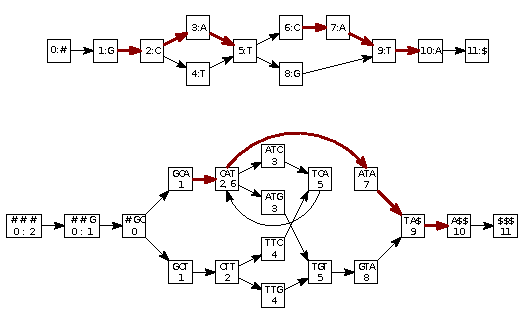
\includegraphics[width=0.8\textwidth]{Chapter2/Figs/sequence_graph_to_DBG.pdf}
  \caption[A sequence graph and its de Bruijn transformation]{
    A sequence graph (top) and its de Bruijn transformation (bottom) for $k=3$.
    The highlighted path in the DBG is a false positive, as it consists of two disjoint paths in the input graph, and is shown to demonstrate the fact that the DBG is not a lossless representation of the input for any length greater than $k$.
    Reprinted from \cite{siren2017indexing}.
  }
  \label{fig:seq_graph_to_dbg}
\end{figure}

To construct the GCSA2 index from variation graph $G$, we transform it into a de Bruijn graph whose nodes are the full set of $k$-length walks through the $G$ (as in figure \ref{fig:seq_graph_to_dbg}) on both strands.
Before doing so, to ensure that all elements of the graph are included in $k$-length paths, we add head and tail nodes labeled $\#$ and $\$$ to the variation graph prior to this transformation.
To maintain the lexicographic ordering invariance required for searching in the GCSA2, we add a special edge connecting these nodes prior to generating our $k$-mer set.\footnote{This can be seen in the LF mapping drawn between $BWT$ and $OUT$ in figure \ref{fig:gcsa2_search}, where a line connects $\$$ with $\#$.}
To allow larger query lengths without direct in-memory enumeration of the full length paths in the source variation graph, GCSA2 uses a series of disk backed steps to double the DBG $k$ until it reaches the desired length.
In practice, it uses four rounds of doubling, beginning with $k=16$, and progressing through $2k$, $4k$, $8k$, and $16k = 256$.
At each step, the DBG is pruned to remove redundancy and reduce memory usage (compare the graph in figure \ref{fig:gcsa2_search} to the DBG in \ref{fig:seq_graph_to_dbg}).
The final FM-index-like model is encoded using succinct data structures from \href{https://github.com/simongog/sdsl-lite}{SDSL-lite} \cite{gbmp2014sea}, with succinct bitvectors used for rare characters like ${\tt N}$, $\$$, and $\#$.

The final GCSA2 data structure model (illustrated in figure \ref{fig:gcsa2_search}) consists of: the $BWT$, which (as in SDBG) represents the edge space of the pruned DBG; $IN$, which marks which edge is the last among the inbound edges to a given node; $OUT$, which marks which edge is the last among the outgoing edges from a given node; and positional samples connecting the DBG nodes with positions in the input graph $G$.
As in the SDBG and GCSA, the nodes of the pruned DBG are not stored, but given implicitly in the number of 1-marked bits in $IN$ and $OUT$.
This can be seen in the relationship between the ``key'' vectors in figure \ref{fig:gcsa2_search} and the $BWT$ vector.
A vector (not shown in figure \ref{fig:gcsa2_search}) $C$ records the lexicographic ranges of the starting characters in the node labels, serving the same purpose as the equivalent vector in the FM-index.
For the index to be useful for graph path queries, we should be able to link lexicographic ranges within the BWT to positions in the original graph.
To do so, we store a set of positional samples as: a vector $B_S$, which indicates those nodes for which we have positional samples; a unary encoding of the number of values stored for each node $B_V$; and the vector of positional samples themselves $V_S$.
Positional samples are stored at the case of branches in the pruned DBG, or at some configurable frequency otherwise.
In linear regions of the pruned DBG, it is possible to use graph DBG graph traversal operations to compute un-sampled positions, thus trading off time and space as is typically done in FM-index implementations on linear strings.

The GCSA2 encoding is highly efficient on real data sets.
When including the suffix tree extensions, GCSA2 uses around 1 bit per $k$-mer in indexes of the 1000GP pangenome graph for $k=128$, which is favorable with comparison to SDBG indexes \cite{siren2017indexing}.
To appreciate the costs of indexing a human genome sized graph\footnote{Precise sizes are given later in the discussion of results.}, the order-256 GCSA2 index of the 1000GP variation graph may be constructed using less than 500GB of scratch space, to and from which are written approximately 3TB during construction, all while requiring less than 50GB of RAM.
This puts GCSA2's indexing resource requirements well within the specifications of standard commodity compute servers.
The resulting index occupies between five and ten times the input graph's serialized size, no more than 50GB for a human genome.
Although it could appear to be a critical limitation, the limit on query length is not a problem in practice.
Few contemporary reads are likely to generate 256bp-long sequences with no mismatch from the reference\footnote{Illumina's reads rarely reach 256bp, and when they do they tend to have higher error rates in the later cycles. The 10-15\% error rate of PacBio and ONT sequencing mean that a 256bp exact match is extremely unlikely, although PacBio circular consensus reads (CCR) may approach this level of accuracy.}, this approach effectively allows us to find all the exact matches for a typical sequencing read.




%To be more precise, we find supermaximal exact matches (SMEMs) as defined in \cite{li2013aligning}.
%The addition of the longest common prefix (LCP) array alongside GCSA2's BWT effectively generalizes all essential operations on a suffix tree to the GCSA2, and enables us to find SMEMs and develop sensitive MEM-based seeding heuristics using the index.



%As an FM-index like structure, GCSA2 supports queries for a pattern $X$ that yield the suffix array interval matching a given pattern: $find(X) = ( sp_{X}, ep_{X} )$, and $locate( sp_{X}, ep_{X} ) = \{ b_1 \ldots b_{count(sp_{X}, ep_{X})} \}$ which yields the positions in the input VG where the given patterns occur.
%The LCP array allows the index to support several operations that require a suffix tree, including $count(sp_i, ep_i)$, which returns the number of matches for a given suffix array range, and $parent(sp_i, ep_i) = (sp_j, ep_j)$, which allows us to traverse the suffix links embedded in the suffix tree and forms the basis of maximal exact match (MEM) inference using GCSA2.

\begin{figure}[htbp!]
  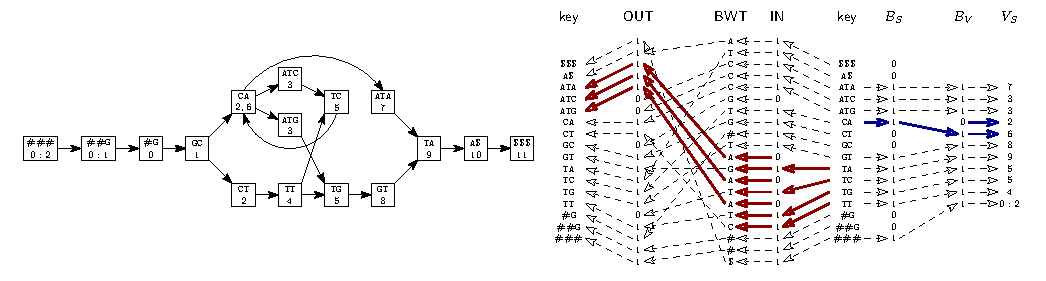
\includegraphics[width=\textwidth]{Chapter2/Figs/DBG_to_GCSA.pdf}
  \caption[Searching in the {\tt GCSA2}]{
    Top: An order-3 pruned de Bruijn graph 3-equivalent to the de Bruijn graph in figure \ref{fig:seq_graph_to_dbg}.
    Bottom: the GCSA2 for the given graph, including both stored elements ($IN$, $OUT$, $BWT$, $B_S$, $B_V$, and $V_S$) and the implicit node sequences shown as the vectors labeled ``key''.
    Not shown, a vector $C$ encodes the number of nodes lexicographically smaller than a given character, supporting backward search and LF-mapping as in the normal FM-index.
    Leftward red arrows illustrate backward searching, showing the steps taken from {\tt T} to {\tt AT}.
    As in algorithm \ref{alg:bwt_find}, the range of nodes beginning with {\tt T} is found from two queries on $C$: $[sp, ep] = [C[T], C[T+1]-1] = [9,12]$.
    The lexicographic range in $BWT$ corresponding to this interval is found by $[select_{IN}(1, sp-1)+1, select_{IN}(1, ep)] = [10,16]$.
    We then apply LF-mapping (as in algorithm \ref{alg:bwt_find}) to find the range in $OUT$ corresponding to the pattern {\tt AT}.
    Finally, rank queries on $OUT$ allow us to convert to a lexicographic range of nodes prefixed by the pattern {\tt AT}, although in this case the mapping is trivial: $[sp,ep] = [rank_{OUT}(1,2),rank_{OUT}(1,4)] = [2,4]$.
    Rightward blue arrows mark the samples belonging to each node, with the blue ones showing them for node {\tt CAT}, which does not correspond to the given backward searching steps, but which would be found by another round of backward searching on {\tt C}.
    Reprinted from \cite{siren2017indexing}.
  }
  \label{fig:gcsa2_search}
\end{figure}

%GCSA2 resolves a number of problems that limit the utility of other graph path indexing schemes.
%Indexing a pruned DBG allows GCSA2 to be applied to arbitrary bidirectional string graphs that include reversals and loops.

\subsection{Haplotype indexes}
%*1.5p 3h*
% worth mentioning gpBWT and PBWT
Recording the path set of a graph in XG (described in section \ref{sec:graph_topology_index}) requires $O(N\overline{P} + {\cal L}|P|)$ space where ${\cal L}$ is the average haplotype length in terms of nodes it crosses, $N$ is the number of nodes in the graph, $|P|$ is the number of paths in the graph, and $\overline{P}$ the average number of paths crossing each node.
Although, such a representation can be compressed, the size of this representation will grow linearly with the addition of new paths, making it impractical as a means to record very large numbers of genomes.

Recording collections of paths is an important requirement for the use of VG in resequencing, as the Markovian property of the bare sequence graph $G = (N, E, P= \emptyset)$ means it can encode exponentially many paths relative to the true input path set used to build the graph.
This introduces significant issues during read mapping and genome inference.
With increasing variant density the number of possible sequence paths of a given length grows exponentially, and this can lead to spurious mismapping (section \ref{sec:1000GP_sim}).
The exponential growth of the path space of the graph has relevance for sequence indexing with GCSA2, and as described in \ref{sec:graph_sequence_indexes}, simplification of the graph in complex regions prior to GCSA2 indexing is required to build indexes in practice.
A haplotype index allows the pruning operation to preserve known haplotypes, rather than defaulting to the reference genome in such cases.
Efficient path indexes could be used for many operations in variant calling and phasing, and may have utility in assembly problems, for instance to losslessly record a read set embedded in a variation graph representing their mutual alignment (section \ref{sec:from_pairwise_alignments}).

Haplotype sequences from the genomes of the same species often share extensive regions of homology, which suggests that they may be very efficiently compressed.
This property was used to store large haplotype sets in the \emph{positional BWT} (PBWT) \cite{durbin2014efficient}.
As input, the PBWT assumes a set of haplotype strings $S_1 \ldots S_m$ of the same length which describe a set of haplotypes relative to a set of variable loci.
$S_j[i]$ records the allele in haplotype $j$ found at locus $i$.
We set $S_j[i] = 0$ when haplotype $j$ has the reference allele at locus $i$, and $S_j[i] > 0$ if it encodes one of possibly several alternate alleles.
The PBWT can be understood as an FM-index of texts $T_1 \ldots T_m : T_j[i] = (i, S_j[i])$ \cite{gagie2017wheeler}.
To search for a haplotype of $h$ in the range $[i,j]$ we look for pattern $h' = (i, h[1]) \ldots (j, h[|h|])$.
The alphabet size of this FM-index is large, but the matrix like structure of the haplotype set means that we can implicitly encode the array indexes by building a separate sub index for each position.
Applying run length encoding to the BWT allows extremely good compression of real haplotype sets.

With the \emph{graph positional Burrows–Wheeler transform} (gPBWT) \cite{Novak2017gPBWT}, we extended this model to work on variation graphs.
The basic model is the same as the generic PBWT except that instead of variant matrix positions we consider haplotype traversals of oriented nodes\footnote{These are described as ``sides'' in \cite{Novak2017gPBWT}.} $n_i$ or $\overline{n_i}$, and rather than a local alphabet of variant alleles we encode a local alphabet $\Sigma_{n_i} = \{ j \in N | e_{ij} \in E \}$ which describes the set of nodes $n_{\{j \in N | e_{ij} \in E \}}$ to which haplotypes continue immediately after the current node $n_i$.
As in the generic PBWT we build an FM-index of $T_1 \ldots T_m$, encoded in what we call the $B_s$ arrays, which provide the local description of prefix sorted haplotypes (equivalently, threads) traversing each node $n_s$.
To deal with the bidirectionality of paths in variation graphs, each haplotype must be encoded in its forward and reverse orientation.
In \cite{Novak2017gPBWT} we demonstrated the expected sublinear scaling of the gPBWT by building an index for chr22 with increasing numbers of samples.
Constructing the gPBWT for haplotype sets representing more than a few hundred samples proved difficult when using our particular implementation.
Progressive construction of the gPBWT in generic graphs was enabled by encoding the gPBWT into dynamic succinct data structures and adding a single haplotype thread and its inverse one at a time.
While functional, we found this to be untenable for large graphs and haplotype sets.
Overheads associated with the dynamic data structures it uses were significant, but the most-difficult issue was the serial nature of the progressive construction algorithm, which gives the algorithm $O(m)$ runtime.
Consequently, all our large-scale experiments were carried out using a partially ordered construction algorithm that worked using a VCF file as input.


\begin{figure}[htbp!]
  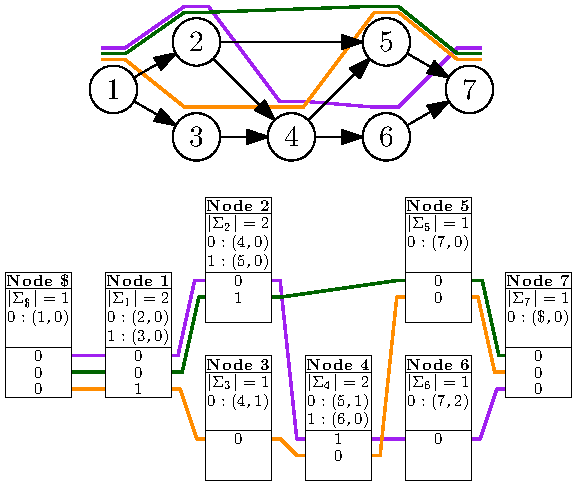
\includegraphics[width=\textwidth]{Chapter2/Figs/gbwt-example.pdf}
  \caption[The Graph Burrows Wheeler Transform]{
    Top: A graph with three paths, each represented as a colored line walking above a series of nodes, where $N={n_1\ldots n_7}$.
    Bottom: GBWT of the paths.
    To build the GBWT we first append a marker node, $n_\$$, to the head of the graph.
    Each node in the GBWT is represented by a record, shown as a white box.
    At the top of each record we find the node identifier, which is implicitly stored in the actual GBWT.
    Each record consists of a local alphabet described in a header and a body consisting of the subset of the full GBWT applying to the given node.
    The alphabet $\Sigma_i$ maps nodes which paths crossing this node reach in their next step into a more compact alphabet.
    It is encoded as a mapping between next node identifier $i$, the local character used to represent that node $\in [0 \ldots |\Sigma_i|)$, and the number of instances of $i$ in the BWTs of all nodes which are lexicographically smaller than the current one.
    For instance, at $n_6$ we find $\Sigma_6 = \{ 0: (7, 2) \}$, because $n_7$ is referred to by the orange and green path crossing the edge $n_5 \to n_7$.
    This arrangement encodes the full BWT in per-node local records.
    We see each path represented as it passes through the BWT record for each node.
    At each node, the sort order of the paths implicitly represented in the BWT reflects the lexicographic sort of their prefixes.
    For instance, at $n_4$, we see $n_{BWT} = [1, 0]$, because the prefix of the purple path before $n_4$ is encoded as $[0,0,0]$, which is lexicographically lower than the prefix of the orange path, $[0,1,0]$.
    Reprinted from \cite{siren2018haplotype}.
  }
  \label{fig:gbwt-example}
\end{figure}

The \emph{graph Burrows-Wheeler transform} (GBWT) \cite{siren2018haplotype} simplifies the data model used by gPBWT so that it is independent of {\tt vg}.
Conceptually, the GBWT can be understood as the FM-index of a transformation of the graph's paths $p_1\ldots p_m \cup \overline{p_1}\ldots \overline{p_m}$ into the text $T = \$( p1 = n_i\ldots n_j) \ldots \$ (\overline{p_m} = \overline{n_j} \ldots \overline{n_i}) $ wherein the paths are rewritten as a series of characters representing node traversals in a large alphabet and delimited by a marker $\$$.
This approach is challenging due to the large size of $T$ for moderately-sized haplotype sets embedded in variation graphs, e.g. $|T| \approx 10^{12}$ for the 1000GP \cite{siren2018haplotype}.
Literally implementing this model would require a large alphabet CSA with suboptimal performance bounds.
Serializing the path set during construction is not feasible, which suggests a dynamic version of the model is required during large scale construction.
Natural variation graphs have a number of properties, such as a manifold partial order, which ca be exploited to improve the memory usage of the GBWT.

In the GBWT we break the full FM-index into per-node records, each of which encodes a header defining an alphabet $\Sigma_{n_i}$ of all the nodes that follow $n_i$ in any path, and a body $BWT_{n_i}$ which is the subset of the full BWT specifying which node follows $n_i$ in each path that passes through $n_i$, with the paths sorted in reverse sequence order up until $n_i$.
Since paths that are similar before $n_i$ tend to be similar after it, this sequence of next node values run length compresses well.

The GBWT supports essential FM-index operations including: $find(X) \to [sp, ep]$ yielding the lexicographic range of suffixes starting with pattern $X$; $locate(sp, ep) \to$ paths occurring in $SA[sp, ep]$; and $extract(j) \to p_j$ which returns the $j$th path in the graph.
By encoding all paths in both orientations, the GBWT can be treated as a kind of FMD-index for haplotypes, allowing bidirectional search.
This means that the GBWT in turn supports MEM-based haplotype matching, which has potential uses in genotype imputation, phasing, association mapping, and other population genetic and evolutionary assays.
Although supported, this particular modality has not yet been explored.

The GBWT representation reflects a number of assumptions that tend to hold for most DNA sequence graphs.
Nodes tend to have low degree, which means the local alphabet size $|\Sigma_{n_i}|$ is small, and we can afford to decompress a small local alphabet encoding efficiently.
Most nodes are not traversed more than once by each path, so the $BWT_{n_i}$ remains small and can be accessed and modified in bounded time.
Due to relatedness among individuals in many species, it is sensible to assume that haplotypes will be highly repetitive, which allows for efficient RLE encoding of $BWT_{n_i}$.
The graph is sorted, and its identifier space has been compacted, which allows us to store the same information for the entire range of node identifiers in bounded memory with respect to $|N|$.
The graph tends to be locally ordered in most places, which decreases the complexity of construction.

A \emph{dynamic GBWT} implementation presents the node records through an index over the range of $[min(i : n_i \in N), max(i : n_i \in N)]$, for each linking to its header, body, incoming edges, and haplotype identifiers.
Construction employs this model in a manner similar to RopeBWT2 \cite{li2014fast}, where batches of paths are insert into the index in a single step following the BCR construction algorithm \cite{bauer2013lightweight}.
This process includes the new paths in the dynamic GBWT by rebuilding each node record affected by the extension.
By breaking the construction process apart for each chromosome and finally merging the compressed GBWTs, it is possible to build the GBWT for the entire 1000GP haplotype set in around 30 hours.
When constructed, the GBWT may be encoded in a compacted but immutable form that uses less memory by representing the per-node model of the dynamic GBWT in a columnar model, for instance concatenating the node BWT vectors and header information for each node each into a single compressed integer vector.
The resulting GBWT requires $\approx 15$ GB, with around half allocated to the GBWT structure itself and half to haplotype identifiers.
The index consumes less than 0.1 bit per node in the stored paths, and we should expect this to improve when we build the GBWT for larger haplotype panels.

\subsection{Generic disk backed indexes}
%*0.5p 0.5h*
\label{sec:generic_disk_backed_indexes}
I began the development of {\tt vg} alone, starting with schemas for the data models, then building an index of the graph using the disk-backed key/value store RocksDB\footnote{\url{https://github.com/vgteam/vg/blob/master/src/index.hpp}}.
I transcribed the data model into namespaces and sorted arrays written into the key/value store.
As compressors of various types could be applied to the sorted arrays backing RocksDB, the memory required for this approach was ultimately similar to that for the final indexing models that I present here.
However, performance was far worse, and the initial version of the aligner based on these systems could not achieve correct results using reasonable amounts of time for large graphs.
Ultimately, this flexible database model has remained important for some pipelines, in particular as a technique to organize alignments against the graph.
Other workloads such as sequence queries were untenable for large genomes, with reliable performance only possible if the entire index of spaced $27$-mers was cached in RAM, requiring nearly 200G in the case of the 1000GP variation graph.
The sorted disk-backed array does have the useful property of allowing prefix queries of the $k$-mer set, but this can easily be attained with GCSA2.
On the networked storage available in my institutional setting, the construction costs for disk-backed index models were usually much worse than those of the XG and GCSA2 models.

\subsection{Coverage index}
\label{sec:coverage_index}

A coverage map, of the alignments to a VG is similar to the labeling required to implement ``colors'' on a DBG \cite{iqbal2012}.
The coverage map loses information about the edge traversals and the paths taken through the graph, which could reduce the visibility of some kinds of variation within it.
But in benefit, this simple model is efficient to use.
The complexity of computing the coverage map is linear in the number of input alignments, and it requires $O(\sum_{\forall{n_i\in N}}|n_i|)$ space to store once built.

I developed an compact coverage index by mapping the sequence space of the graph into a vector and recording coverage across it for a GAM read set.
During construction, a succinct format is employed to store each base's coverage in a single byte as long as it is below 255, and in a secondary hash table if it reaches or exceeds 255.
Finally, a compressed integer vector is generated, which can be queried by graph position computed from the XG index of the graph.
I extended this concept with a succinct ``pileup'' format \cite{li2009sequence} generated from the edits against the graph.
In this model edits in mappings which don't match the reference were serialized into a byte alphabet using Protobuf, such that each non-reference edit $e_j$ at position $b_i$ was recorded as a string $\$b_i e_j$, with the idea that by building a CSA/FM-index from these I could obtain the set of edits at each graph position through pattern matching.
However, I found it impossible to construct this for a large high-coverage sequencing sample, and have not continued this line of investigation.

\section{Sequence alignment to the graph}
%*0.5p 0.5h*
To align sequences to a VG, we use the graph and sequences indexes described in the previous section (\ref{sec:index_structures}) to derive MEMs between a query and the graph.
A weighted DAG collinear chaining model is built from the MEMs which respects their relative positions in the graph and the read, favoring collinear mappings of MEMs, and a max-sum DP algorithm is applied to this alignment DAG to extract likely mappings based on the MEMs.
We then align the sequence locally to the graph at each of the high scoring chains using various sensitive alignment algorithms that use various kinds of dynamic programming.

To detect structural variation and align long reads without incurring quadratically-scaling computational penalties, we apply a kind of banding and a second layer of chaining.
In \emph{chunked alignment}, large sequences are broken up into overlapping segments, each of which is aligned individually in any order or orientation.
This subdivision provides a kind of banding to the alignment algorithm, preventing the evaluation of the full DP matrix, but more importantly it also allows alignments that are generated to represent any kind of variation.
Each chunk is aligned independently.
The same collinear chaining model, with different parameters, is used to establish the optimal global chain through the alignment chunks, thus yielding a full alignment for an input sequence of any size.
Where our reads are shorter than the standard chunk size (256bp), the alignment behaves exactly as in {\tt bwa mem}.
Figure \ref{fig:alignment_to_cactus_yeast} illustrates the alignment of a long read against a complex graph.

\emph{Unfolding} and \emph{DAGification} transform a cyclic bidirectional sequence graph with inversions to an acyclic simple sequence graph one in which all $k$-paths in the first graph are represented.
Any alignment algorithm that may be implemented on a sequence DAG can thus be used.
Optionally, other alternative DP alignment algorithms implementing a banded global alignment can be applied, and I describe one of these that I implemented to \emph{surject} alignments into a particular reference path.

\begin{figure}[htbp!]
\centering
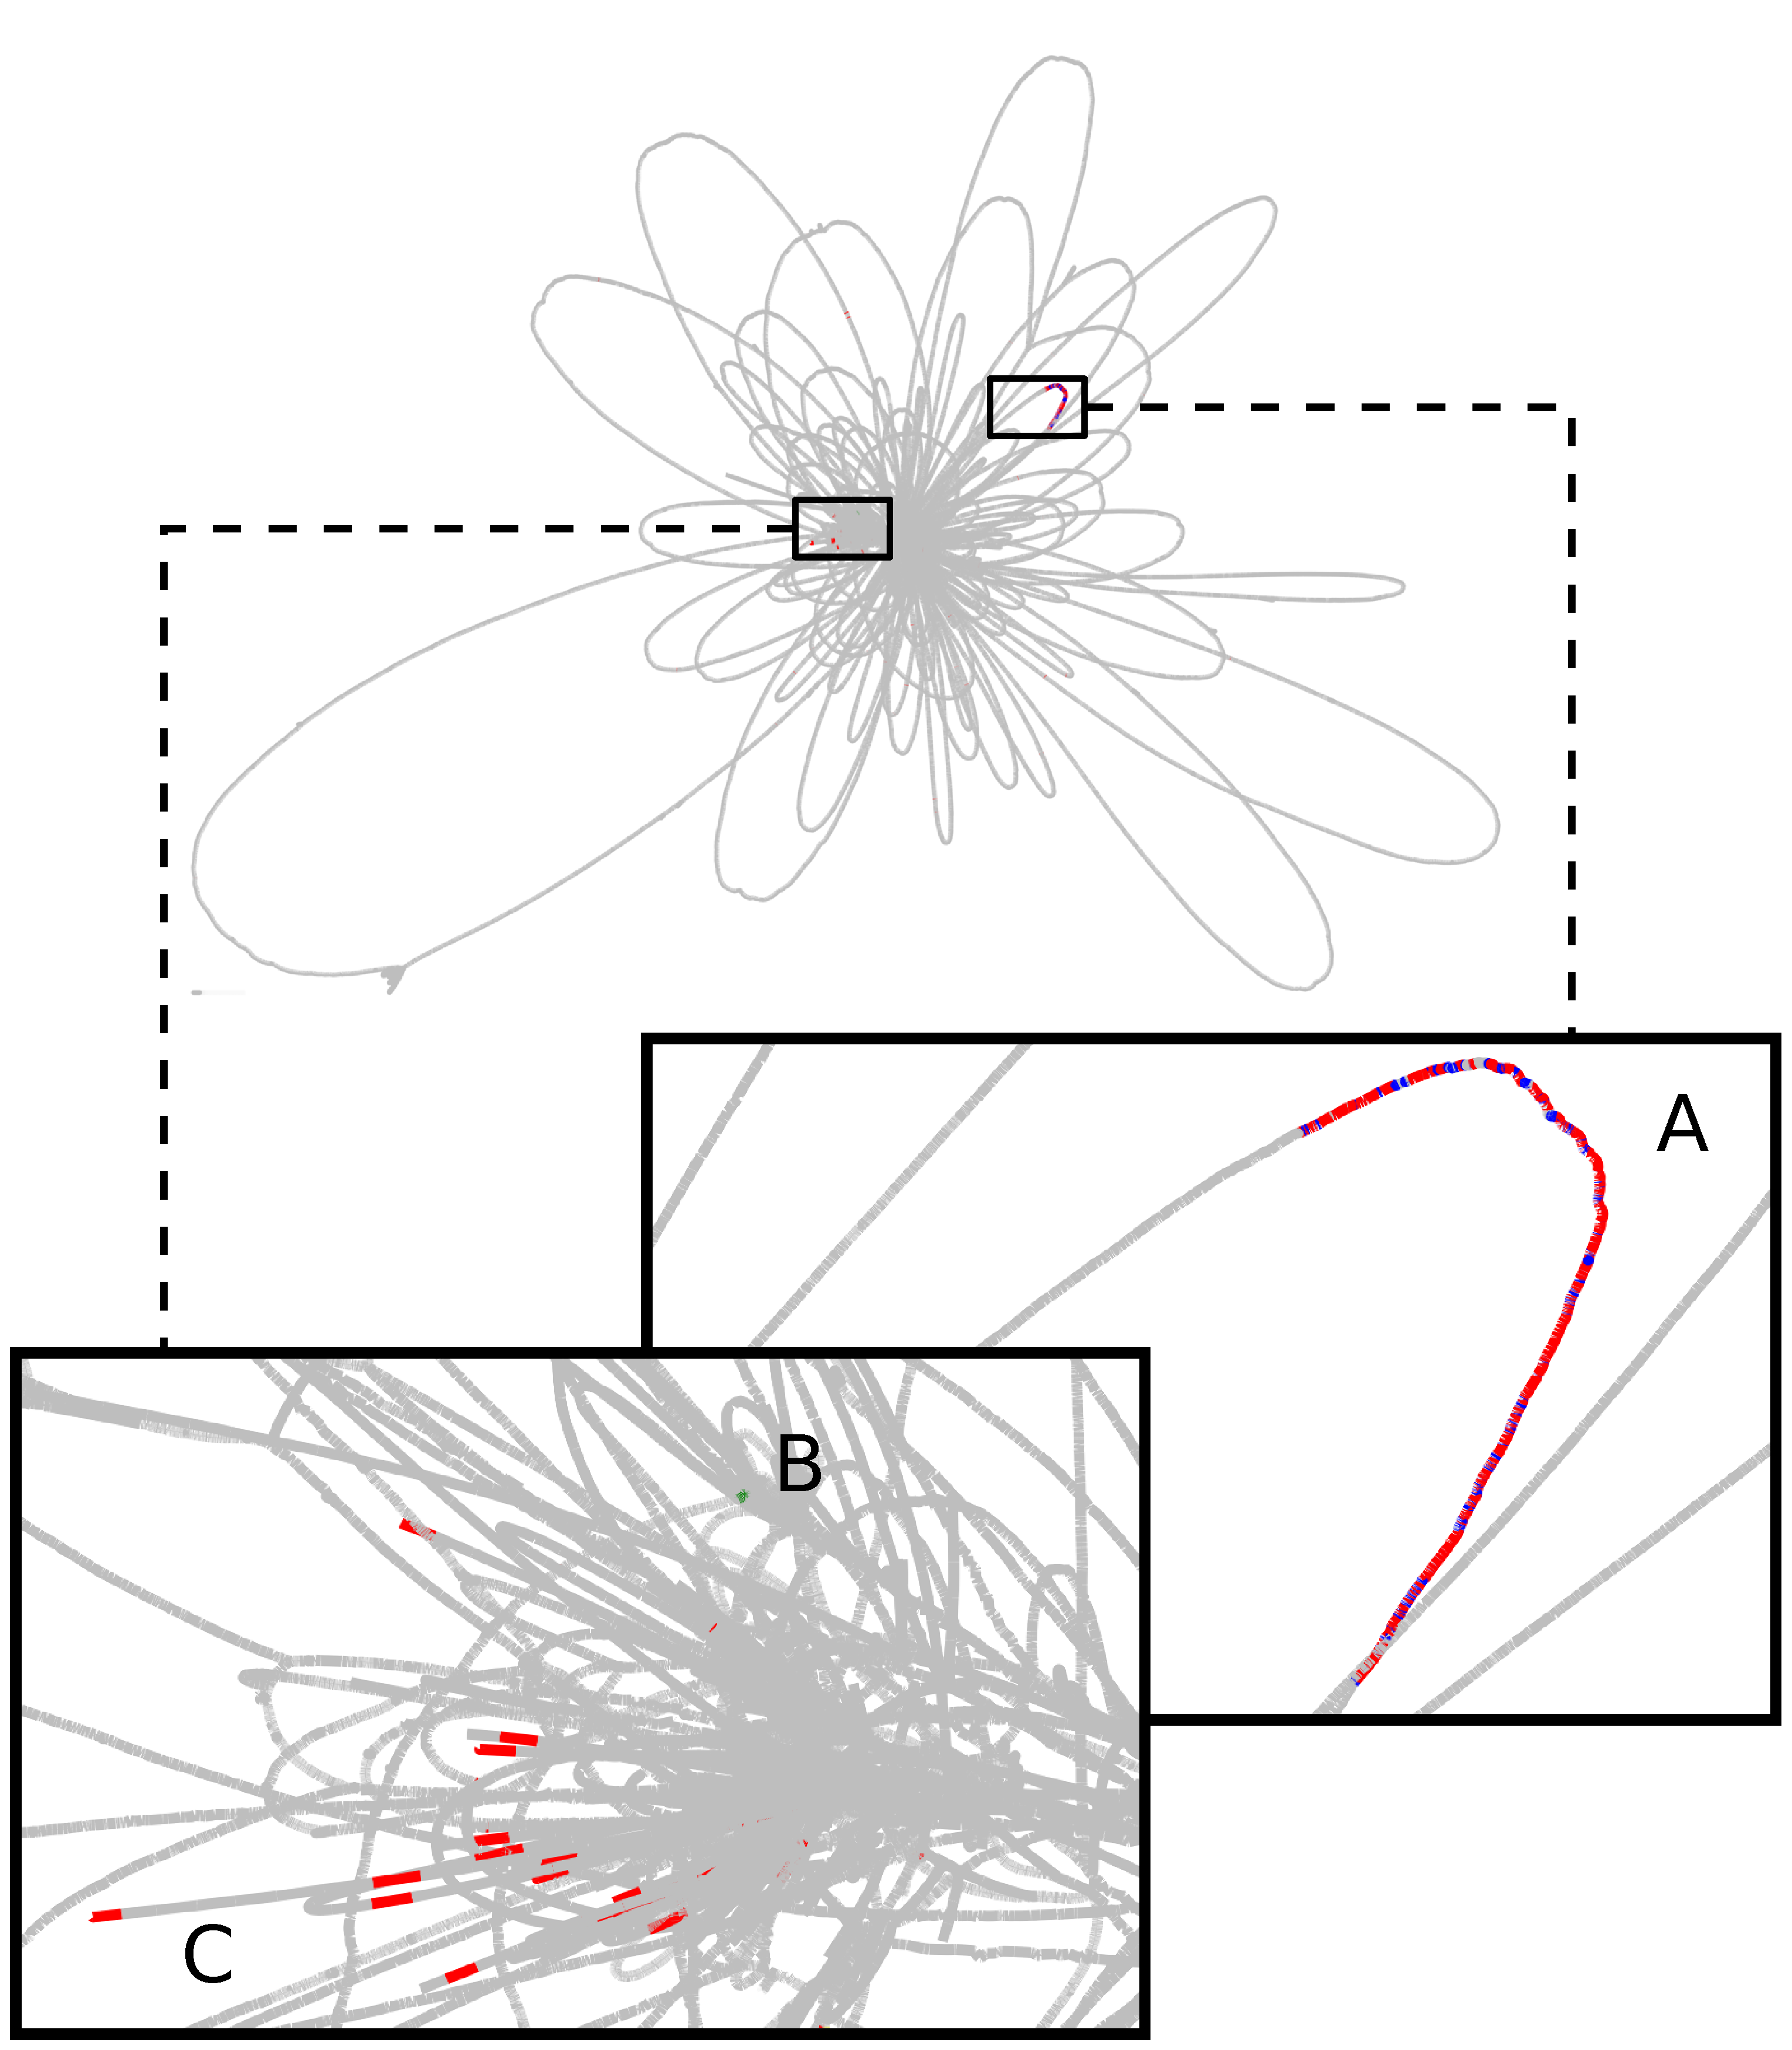
\includegraphics[width=1.0\textwidth]{Chapter2/Figs/mapping_cactus_pacbio_aln_vizzy.pdf}
\caption[Alignment of a PacBio read to a yeast pangenome]{
  Aligning a 32,737bp PacBio read from the SK1 strain to a yeast pangenome graph (section \ref{sec:yeast_cactus}).
  Red nodes contain initial MEM hits, while other nodes are colored if they were matched during local alignment.
  (A) The nodes found in the best alignment are labeled in blue.
  (B) A much smaller secondary alignment is shown in green.
  (C) MEM hits for this read cluster in chromosome ends, which are seen as tips in the graph visualization.
}
\label{fig:alignment_to_cactus_yeast}
\end{figure}


\begin{figure}[htbp!]
\centering
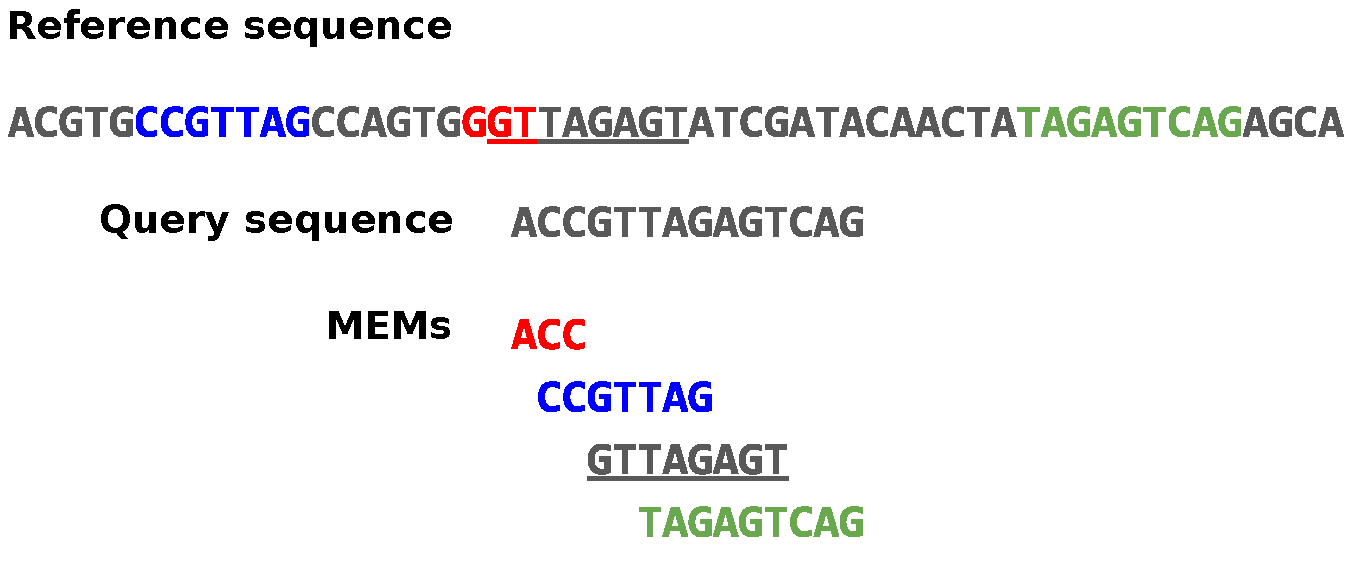
\includegraphics[width=0.8\textwidth]{Chapter2/Figs/mem-finding.pdf}
\caption[Finding maximal exact matches (MEMs)]{
  Maximal exact matches (MEMs) found by the application of algorithm \ref{alg:mem_find} to the given query sequence and a GCSA2 index built from the shown reference sequence.
  MEMs are listed below the query sequence with colors that match their matching location in the reference sequence.
  Note that one MEM is found on the reverse strand of the reference ({\tt ACC} matches {\tt GTT}).  
}
\label{fig:mem_finding}
\end{figure}


\subsection{MEM finding and alignment seeding}
%*2p 2h*
A set of super-maximal exact matches (SMEMs) of a query sequence are generated by backward search in the GCSA2 index.
When backward search breaks, we step back to the last matching interval and use the suffix tree extension of the index to obtain the parent node of this interval.
The GCSA2's {\tt LCPArray} extension allows interrogation of the suffix tree structure, which in turn this allows us to remove the invariant sequence from the end of our previous matched range and continue search for the next maximal match.
Algorithm \ref{alg:mem_find} provides a sketch of this process as it relates to the GCSA2 FM-index encoding and LCPArray.

Not shown in this algorithm sketch are a series of ``reseeding'' passes whereby long MEMs are used as the basis for further exact match finding, but with a maximum limit to the detected match size.
When backward search yields an exact match of this size, we use the same suffix tree operation to reset our match range with the next possible match.
This reseeding operation is required to obtain high sensitivity via MEM based alignment seed lookup.
At sufficient frequency to frustrate our mapping sensitivity in real genomes, a long MEM can mask out shorter sub-matches that might be contained within it, and which correspond to the correct mapping location.
The resulting MEMs are not super-maximal, thus we tend to call these heuristically derived exact matches ``MEMs'' for simplicity.

%the suffix tree encoded in the GCSA2 index until the count of matching strings drops to 0, then backing off one step to find all longest exact matches.
%A recursive series of ``reseed'' passes through the traversal can then identify distinct next-longest matches which are used both to improve sensitivity.

We use MEMs to seed alignments in {\tt vg}.
As indicated in algorithm \ref{alg:mem_find}, the GCSA2 index supports lookup of matches by position in the original graph.
In conjunction with a distance estimator, these positions are used to build a collinear chaining model that allows us to estimate likely subgraphs matching our query (described subsequently in section \ref{sec:collinear_chaining}).
Chains of MEMs that are consistent with a mapping between the query sequence and the graph are found using a weighted graphical model in which the optimal alignment is likely to form a max-sum path.
For each candidate chain, we then locally align the read against the graph. 
Scoring results from the local alignment are used to rank the candidate alignments.
We then return the best alignment, or multiple candidates if multiple mappings are required, with calculation of mapping quality used to provide an estimate in our confidence in the best alignment (section \ref{sec:mapping_quality}).

\begin{algorithm}
  \caption[MEM finding]{
    Finding maximal exact matches using the GCSA2 suffix tree extension
  }
  \label{alg:mem_find}
  \begin{algorithmic}
    \Function{FindMEMs}{Q} \Comment{Find the MEMs for the given query sequence $Q$}
    \State $mems \gets \emptyset$ \Comment{The list of MEMs that we'll return}
    \State $c \gets Q[|Q|-1]$ \Comment{Current character in our search}
    \State $sp \gets C[c]$ \Comment{Beginning of our SA interval}
    \State $ep \gets C[c+1]-1$ \Comment{End of our SA interval}
    \State $mem.begin \gets |Q|-2$ \Comment{Build up a MEM structure to store our current match}
    \State $mem.end \gets |Q|-1$ \Comment{Record the current matching interval}
      \For{$i \in [|Q|-2 \ldots 0]$} \Comment{Step backwards through the string}
        \State $last = [sp, ep]$ \Comment{Store the last range, in case search breaks}
        \State $c \gets Q[i]$ \Comment{Update our character}
        \State $sp \gets C[c] + rank_{BWT}(c, sp - 1)$ \Comment{Update $sp$ dependent on $c$}
        \State $ep \gets C[c] + rank_{BWT}(c, ep) - 1$ \Comment{Do the same for $ep$}
        \If{$sp > ep$} \Comment{The current extension has failed}
          \State $mem.begin \gets i + 1$ \Comment{Remove the last (unmatched) character}
          \State $mem.range \gets last$ \Comment{Set the range to the last matching range}
          \State $mem.positions \gets GCSA2.locate(mem.range)$ \Comment{Get MEM positions}
          \State $mems.append(mem)$ \Comment{Store the last MEM for return}
          \State $p \gets LCP.parent(last)$ \Comment{Get the suffix tree node parent of the last range}
          \State $mem.end \gets mem.begin + p.lcp()$ \Comment{Remove the common prefix}
          \State $[sp, ep] \gets p.range()$ \Comment{Use the SA range of the suffix tree parent node}
        \EndIf
        \EndFor
      \State $mems.append(mem)$ \Comment{Add the last MEM to the MEMs to return} \\
      \Return{$mems$} \Comment{Return the MEMs we've found}
    \EndFunction
  \end{algorithmic}
\end{algorithm}

\subsection{Distance estimation}
\label{sec:distance_estimation}
%*1p 1h*
To cluster our MEMs we require a distance function that returns the minimum distance between any two positions $dist(b_i, b_j)$. % \to \min_{\forall p \in N \times N}{|p|} : pos(p[1]) = b_i \land pos(p[|p|]) = b_j$.
Distance measurement between nodes in a variation graph is non-trivial, with exact solutions to the problem theoretically requiring $O(E \log \log L)$ where $L = \max_{\forall n_i \in N} |n_i|$ is the maximum node length \cite{karlsson1983mlog}.
Precomputation of the full set of distances would thus require $O(N^2 E \log \log L)$ time and $O(N^2)$ space, which is infeasible for any large graph.
Many variation graphs are mostly linear, which we can exploit to build an approximate distance metric.
Provided we have applied a partial sort to the graph, in the partially ordered regions we can use the offset of each node in the XG sequence vector $S_\textbf{iv}$ as an approximate 1D coordinate, which we query using the corresponding rank/select dictionary $S_\textbf{bv}$.
We expect that in much of the graph $S_\textbf{bv}^{select_1}(id(b_j))+\mbox{offset}(b_j) - S_\textbf{bv}^{select_1}(id(b_i))+\mbox{offset}(b_i) \propto dist(b_i, b_j)$, where $id(b)$ is the function that returns the rank of position $b$'s node in the XG index, and $\mbox{offset}(b)$ returns the position's offset inside the sequence label of the node.

Nonlinearities in the graph will frustrate this metric, and to manage these we rely on the positional index provided by the \emph{positional paths} given in the XG index.
In these, we can query the relative positions of nodes in the path in $O(1)$ time.
Where both positions are not on the same path, we use a bounded local exploration of the graph near our positions $b_i$ and $b_j$ to attempt to find anchoring nodes on the same path.
In our clustering step (section \ref{sec:collinear_chaining}) we consider the multiple coordinate systems to develop a global pseudoalignment.

\subsection{Collinear chaining}
%*0.5p 0.5h*
\label{sec:collinear_chaining}

In most cases, single MEMs do not cover the full read length, so we need to combine information from multiple MEMs to determine a candidate mapping location.
It is impractical to attempt a full DP based alignment at each MEM location, and instead, we apply a heuristic approach wherein a model is built with the available MEM seed information, their graph positions, their positions in the query sequence, and the scoring parameters used for local alignment.
The \emph{MEM Chain Model} is a DAG, $G_\textsc{MemChain} = (N, E)$, in which each node $n_i \in N$ derives from a MEM, and each edge $e_{ij} \in E$ to represent a possible transition between MEMs that we may find in an alignment.

\begin{figure}[htbp!]
\centering
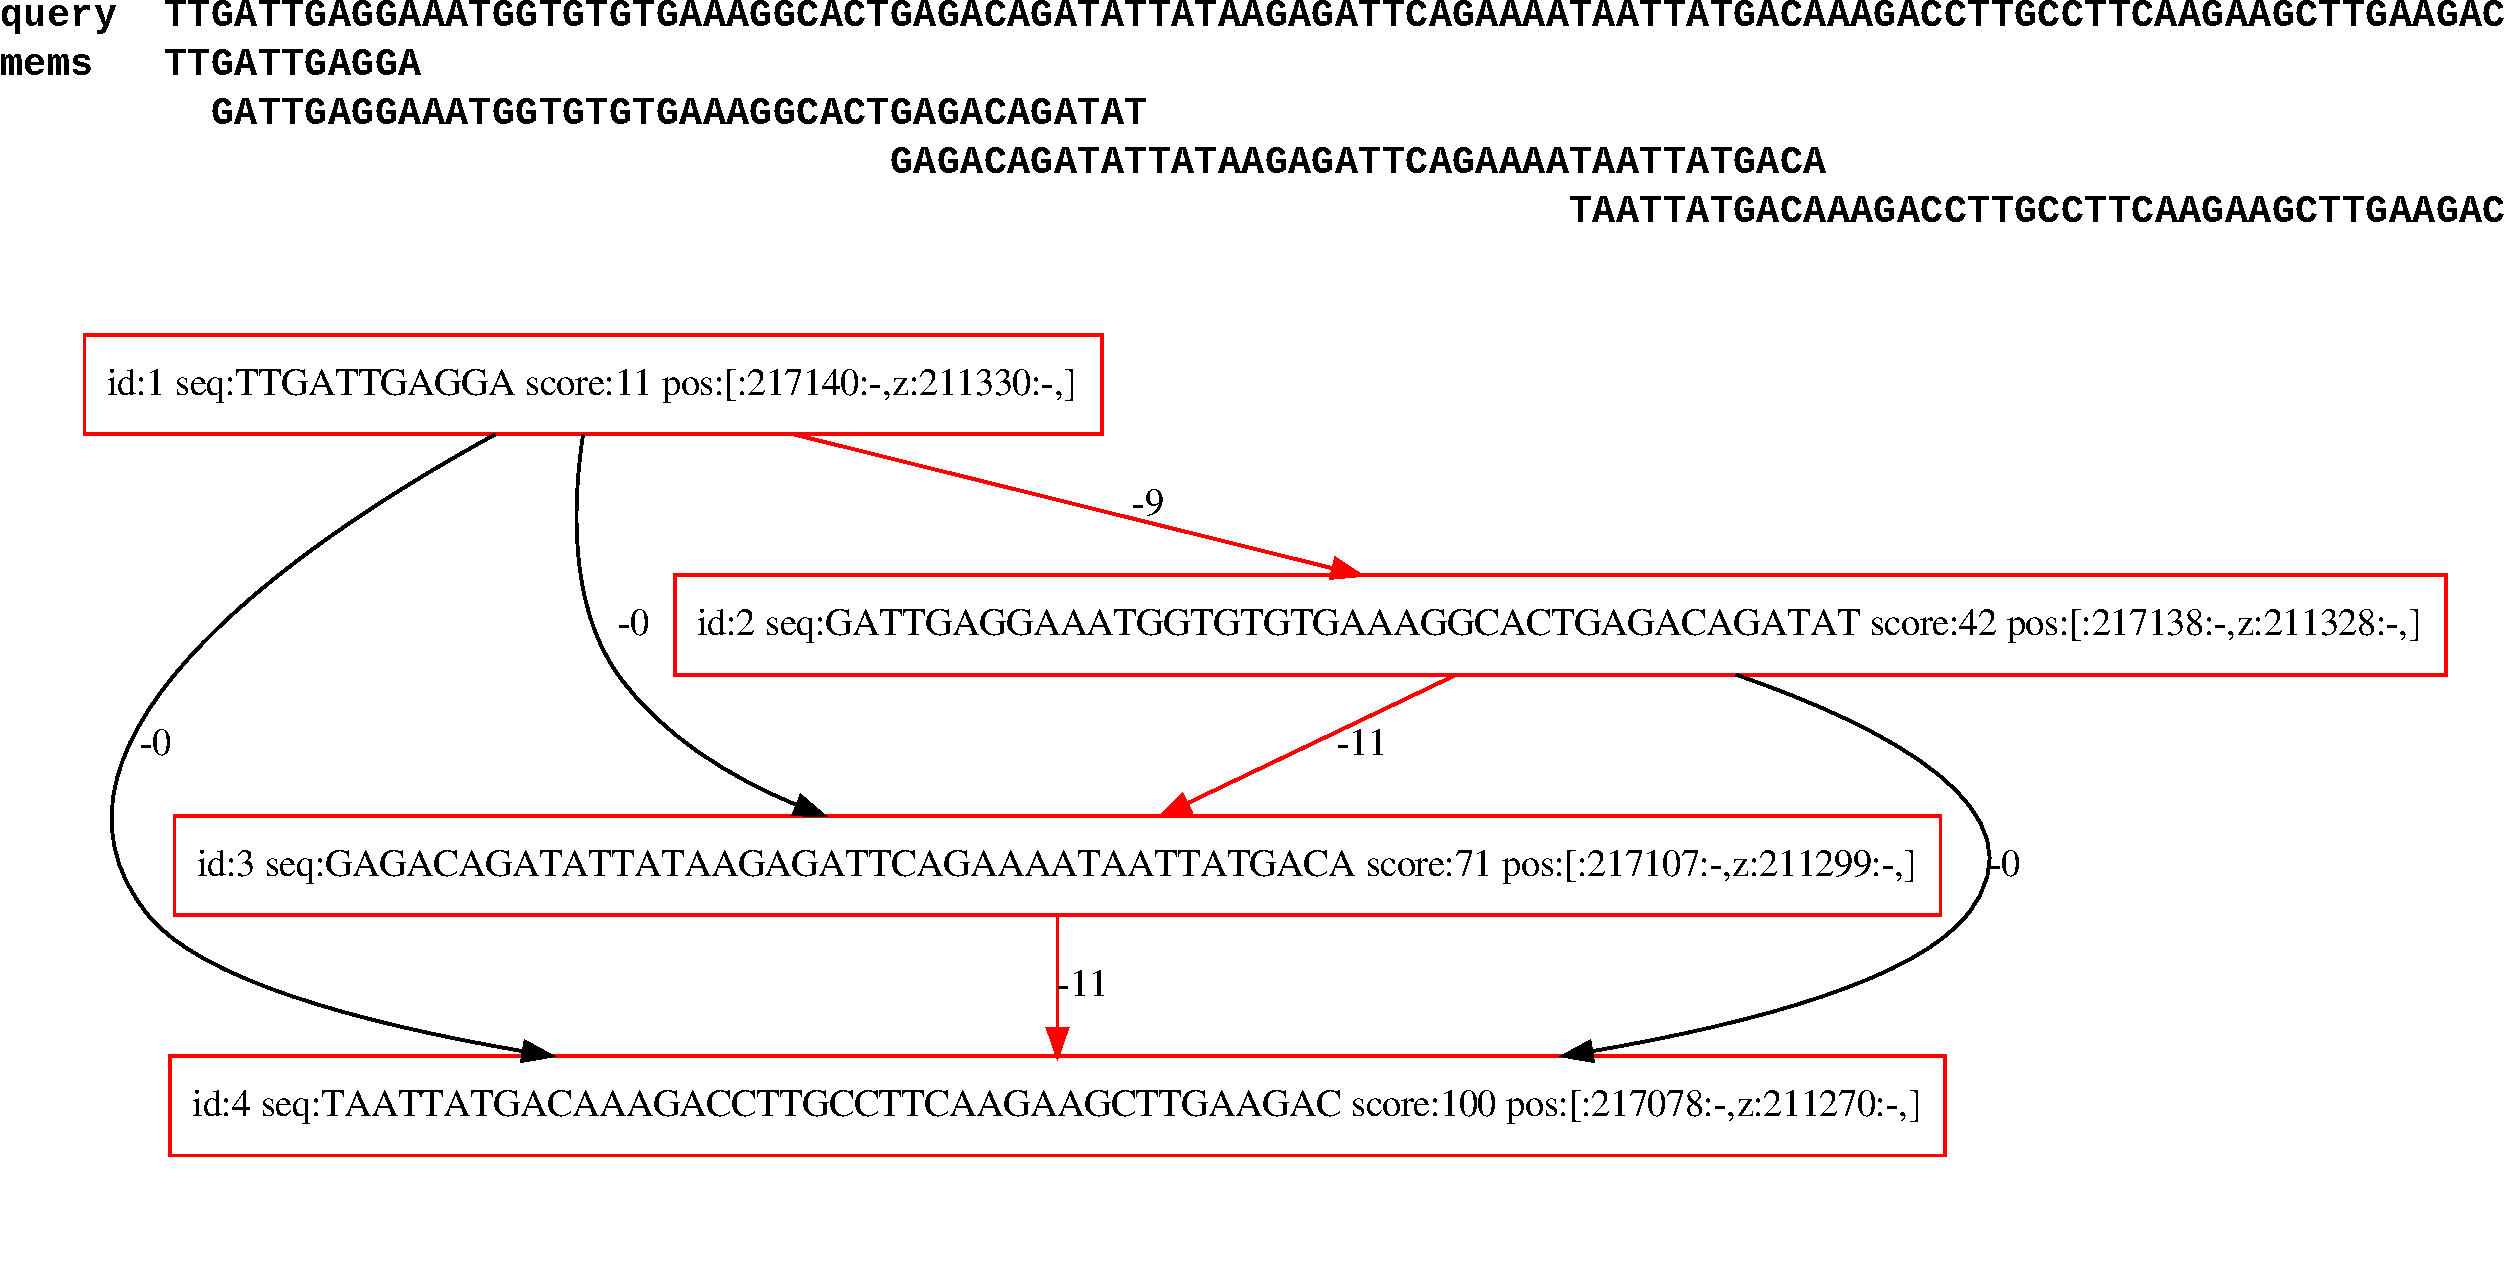
\includegraphics[width=1.0\textwidth]{Chapter2/Figs/memchain_dag.pdf}
\caption[The MEM Chain Model]{
  Establishing collinear chains of MEMs to drive sequence read mapping.
  Above: a set of MEMs derived from a perfect read simulated from a 1Mbp test region from the 1000GP graph of chr20, using a maximum MEM length of 40bp to generate multiple MEMs for exposition.
  Below: the first evaluation of the MEM Chain Model for this set of MEMs.
  The model is shown in full, with the scores established as described in the text.
  Each node refers to a single MEM, its positions in the graph, and the score derived from the first pass of the max-sum algorithm.
  A weight is applied to each node equal to the length of its sequence times the match score used in local alignment.
  A score on each edge is computed as the gap open and extension score implied by the difference in distance between the MEMs in the read and in the graph positions, minus the overlap length of the MEMs in the read.
  The maximum scoring chain is shown in red.
}
\label{fig:memchain_model}
\end{figure}

Each $n_i$ has a starting position in the query $mem\_pos(n_i)$ and a length $mem\_length(n_i)$.
To estimate the alignment score that we would achieve by using this MEM in an alignment, we add a weight ${\cal W}_{n_i}$ to each node that scales this length by the match score used in local alignment $\omega_\textbf{match}$:

\begin{equation}
  {\cal W}_{n_i} = mem\_length(n_i) \omega_\textbf{match}
\end{equation}

Each $n_i$ also has an associated set of graph positions $graph\_pos(n_i) = \{ b_1 \ldots b_m \}$.
Edges $e_{ij}$ in $G_\textsc{MemChain}$ represent possible transitions between MEMs, and are weighted (${\cal W}_{e_{ij}}$) by the minimum estimated distance between the given graph positions for each MEM, times the gap open and extension costs, less the overlap between the MEMs in the read times the match score:

\begin{equation}
  dist_{e_{ij}} = \min_{dist(b,d)} \forall b \in graph\_pos(n_i), \forall d \in graph\_pos(n_j)
\end{equation}

\begin{equation}
  cost_{e_{ij}} = \omega_\textbf{extend} dist_{e_{ij}} + \omega_\textbf{open} [dist_{e_{ij}} \ne 0]
\end{equation}

\begin{equation}
  overlap_{e_{ij}} = (mem\_pos(n_i) + mem\_length(n_i)) - mem\_pos(n_j)
\end{equation}

\begin{equation}
  {\cal W}_{e_{ij}} = cost_{e_{ij}} - overlap_{e_{ij}} \omega_\textbf{match}
\end{equation}

If we are establishing $G_\textsc{MemChain}$ based on MEMs derived from a read pair, and $n_i$ and $n_j$ are in different fragments in the read pair, then we derive ${\cal W}_{e_{ij}}$ based on a weight related to the probability of $dist_{e_{ij}}$ under an observed fragment length distribution:

\begin{equation}
  {\cal W}_{e_{ij}}^{\textsc{paired}} = P(dist_{e_{ij}} | obs\_frag\_len)
\end{equation}

These node and edge weights relate to the alignment score that we would obtain by passing through a series of MEMs.
We expect a positive score due to an exact match, so we apply a positive weight to each node as it represents a MEM.
Transitions between MEMs may encode gaps or mismatches.
We cannot estimate mismatch counts for the read from the set of MEMs obtained for our query, but we can use our position index and the function $dist(b,d)$ to estimate gap lengths.
We take the score of a pseudoalignment ${\cal P} = n_i \ldots n_j$ in the model to be:

\begin{equation}
  {\cal S}_{\cal P} = \sum_{i = 0}^{|{\cal P}|-2} {\cal W}_{{\cal P}[i]} + {\cal W}_{e_{{\cal P}[i]{\cal P}[i+1]}}
\end{equation}

Given this definition, we expect the maximum sum walk ${\cal P}_\textsc{max} = n_i \ldots n_j$ through the graph to be likely to yield the series of MEMs and graph positions involved in the maximum scoring alignment.
This pseudoalignment is approximate due to the incompleteness of our score estimate and the fact that our MEM set is not guaranteed to capture the optimal alignment.
To obtain a precise score we must then locally align the query against the graph.

To use $G_\textsc{MemChain}$ to drive alignment, we need to be able to use it to derive a series of candidate alignment locations.
We do so by applying a standard max-sum dynamic programming approach to $G_\textsc{MemChain}$.
In this process, we derive a score for each node, ${\cal S}_{n_i}$, as the sum of own weight, the maximum score of any previous node, and the weight of the edge connecting the maximum scoring inbound node and the current node.

\begin{equation}
  {\cal S}_{n_i} = {\cal W}_{n_i} + \max_{\forall e_{ji} \in E} \left( {\cal W}_{e_{ji}} + {\cal S}_{n_j} \right)
\end{equation}

To allow traceback of the maximum scoring path, we record the maximum inbound node for each node.

\begin{equation}
  {\cal T}_{n_i} = \operatorname*{argmax}_{n_j} \left( {\cal W}_{e_{ji}} + {\cal S}_{n_j} \right)
\end{equation}

At the end of the scoring phase, we find the highest scoring node.

\begin{equation}
  n_{max} = \max_{\forall n_i \in N} {\cal S}_{n_i}
\end{equation}

Walking back through the series of recorded traceback pointers yields the maximum scoring path under the model.
We define the series of nodes in the max-sum path by $n_{max-i-1} = {\cal T}_{n_{max-i}}$.
The resulting path is expressed in reverse order relative to our traceback.

\begin{equation}
  {\cal P}_\textsc{max} = n_{max-|{\cal P}_\textsc{max}|} \dots n_{max-1}, n_{max}
\end{equation}

To obtain a series of candidate alignments, after each pass of max-sum, we mask out the set of nodes and edges traversed by our last optimal path, run the scoring phase without these MEMs, and finally derive the next-best traceback.


Although the exact algorithm is different, in spirit our implementation is similar to that developed in \cite{kuosmanen2018using}, which extends collinear chaining to DAGs by running a similar model over a minimal set of paths covering the graph.


%In this model the nodes correspond to the reference graph positions where MEMs in the read occur and the transitions between nodes correspond to a weight that is proportional to the indel size implied by the difference in distance between the positions of the MEMs in the read and their distances in the graph. 
%To allow us to consider different distances calculated from different positional paths, we record one node per positional path that each MEM touches.
%If we are aligning a read pair, the weight between MEMs on different fragments is proportional to the probability of that distance under a learned model of the fragment insert size distribution. 
%Once we establish this model, we take the Viterbi path through it as our first candidate alignment. 
%By masking out the states in this path and re-running the Viterbi algorithm on the model, we can extract a series of candidate alignments in descending order of goodness. 




\subsection{Unfolding}

Every node has an implicit default orientation so that it is possible to determine edges that cause an inversion, i.e. those which connect between a forward and a reverse complement node orientation. 
When \emph{unfolding} the graph, we use a breadth first search starting at every inverting edge in the graph to explore the reverse complemented portions of the graph that we can reach within length $k$ from the inverting edge.
We then copy this subgraph, take its reverse complement, and replace the inverting edges connecting it to the forward strand of the graph with non-inverting ones.
If $k$ is as long as the longest walk in the graph, then unfolding will render the forward and reverse complement of the original graph on the forward strand of the unfolded graph.

\subsection{DAGification}
\label{sec:DAGify}

Variation graphs may have cycles.
These are useful as compact representations of copy number variable regions, and arise naturally in the process of genome assembly.
However, partial order alignment algorithms do not handle these structures, and so we convert cyclic graphs into $k$-path equivalent acyclic form in order to apply DAG-based alignment algorithms to them.
To do so, we unroll cyclic structures by copying their internal nodes an appropriate number of times to allow a given query length to align through the unrolled version of the component.
If our query is shorter than this limit, $k \geq |Q|$, then we are guaranteed to find the optimal alignment in the original graph by aligning against the DAGified one.

We first detect all strongly connected components by using a recursion-free implementation of Tarjan's strongly connected components algorithm \cite{tarjan1972depth}.
Then, we copy each strongly connected component and its internal edges into a new graph.
We greedily break edges in this graph that introduce cycles.
Next we $k$-DAGify the component progressively copying the base component and, for each edge between nodes in the component, connecting from the source node in the previous copy to the target node in the current copy.

We use dynamic programming to track the minimum distance back through the graph to a root node outside the component at each step.
When this reaches our target $k$, we stop unrolling, and add the expanded component back into the graph by reconnecting it with its original neighborhood.
For each copy of a node in the DAGified component we copy all its inbound and outbound edges where the other end of the edge lies outside the strongly connected component.
The resulting graph is acyclic and supports queries up to length $k$ on the original graph using a translation that we maintain between the new graph and the source one.

\begin{figure}[htbp!] 
  \centering
  \begin{subfigure}[t]{0.49\textwidth}
    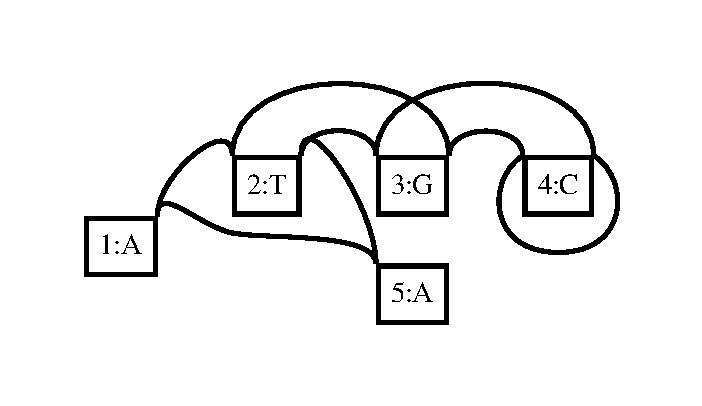
\includegraphics[width=1.0\textwidth]{Chapter2/Figs/loopy_dagify0.pdf}
    \caption{$k=0$} \label{subfig:dagify_k0}
  \end{subfigure}
  \begin{subfigure}[t]{0.49\textwidth}
    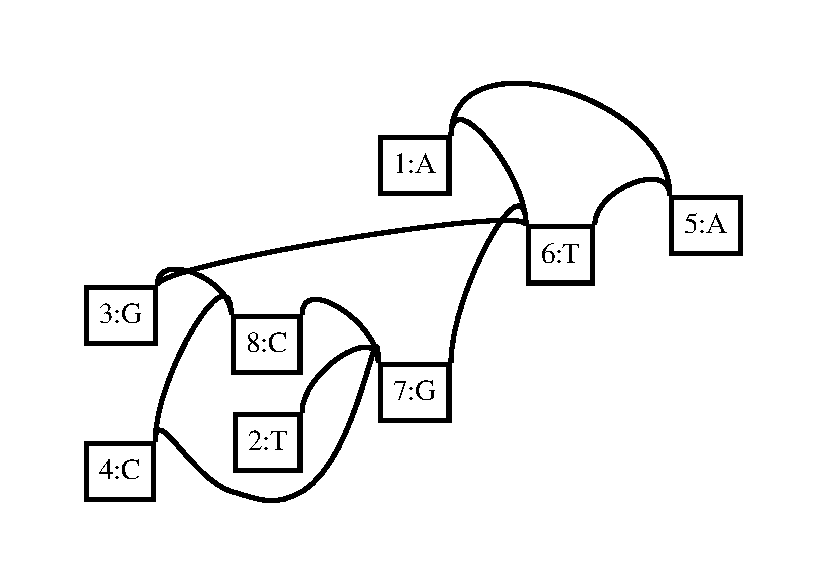
\includegraphics[width=1.0\textwidth]{Chapter2/Figs/loopy_dagify1.pdf}
    \caption{$k=1$} \label{subfig:dagify_k1}
  \end{subfigure}
  \begin{subfigure}[t]{0.49\textwidth}
    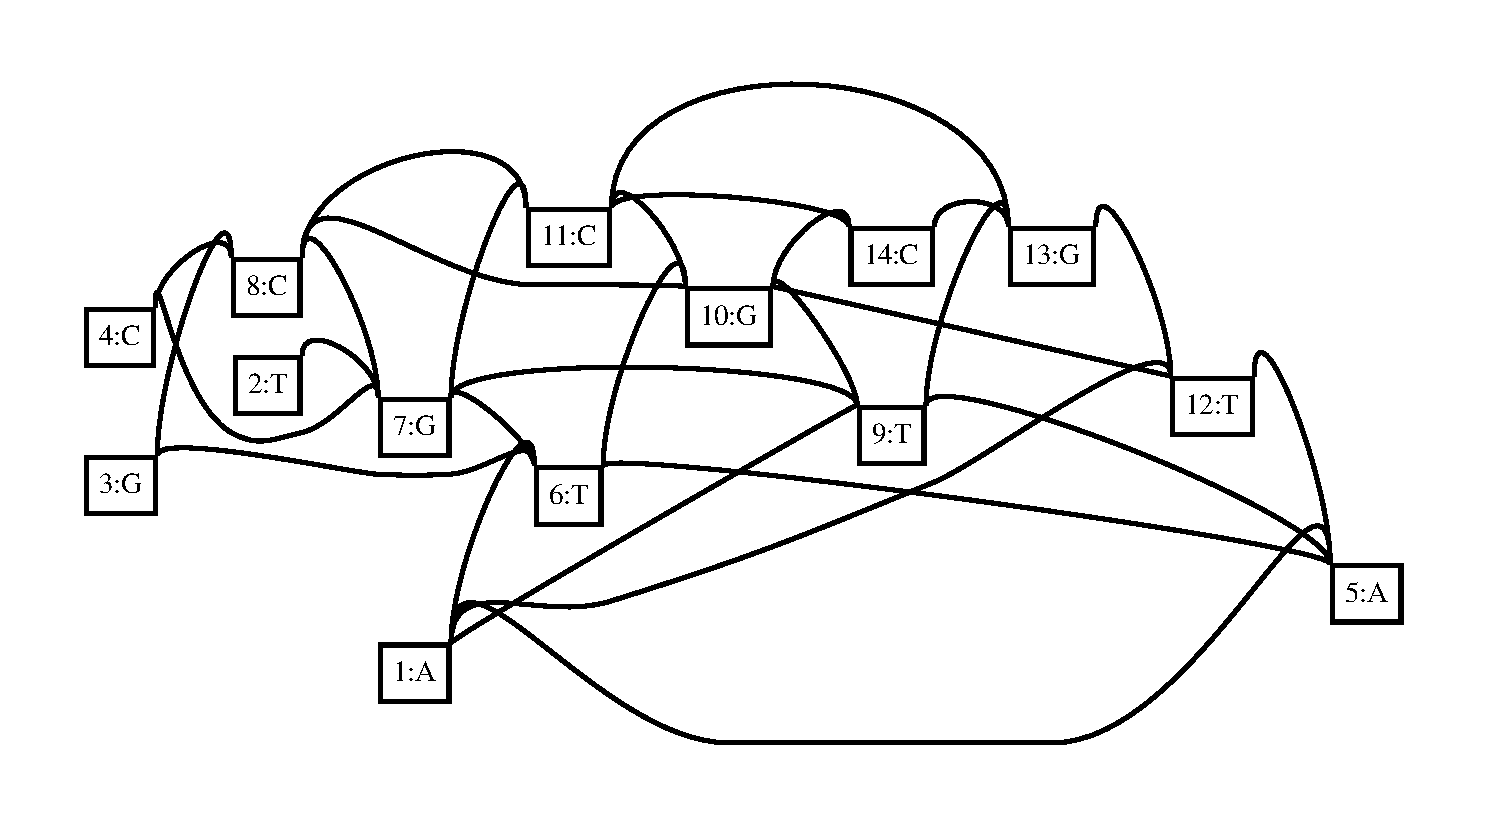
\includegraphics[width=1.0\textwidth]{Chapter2/Figs/loopy_dagify4.pdf}
    \caption{$k=4$} \label{subfig:dagify_k4}
  \end{subfigure}
  \begin{subfigure}[t]{0.49\textwidth}
    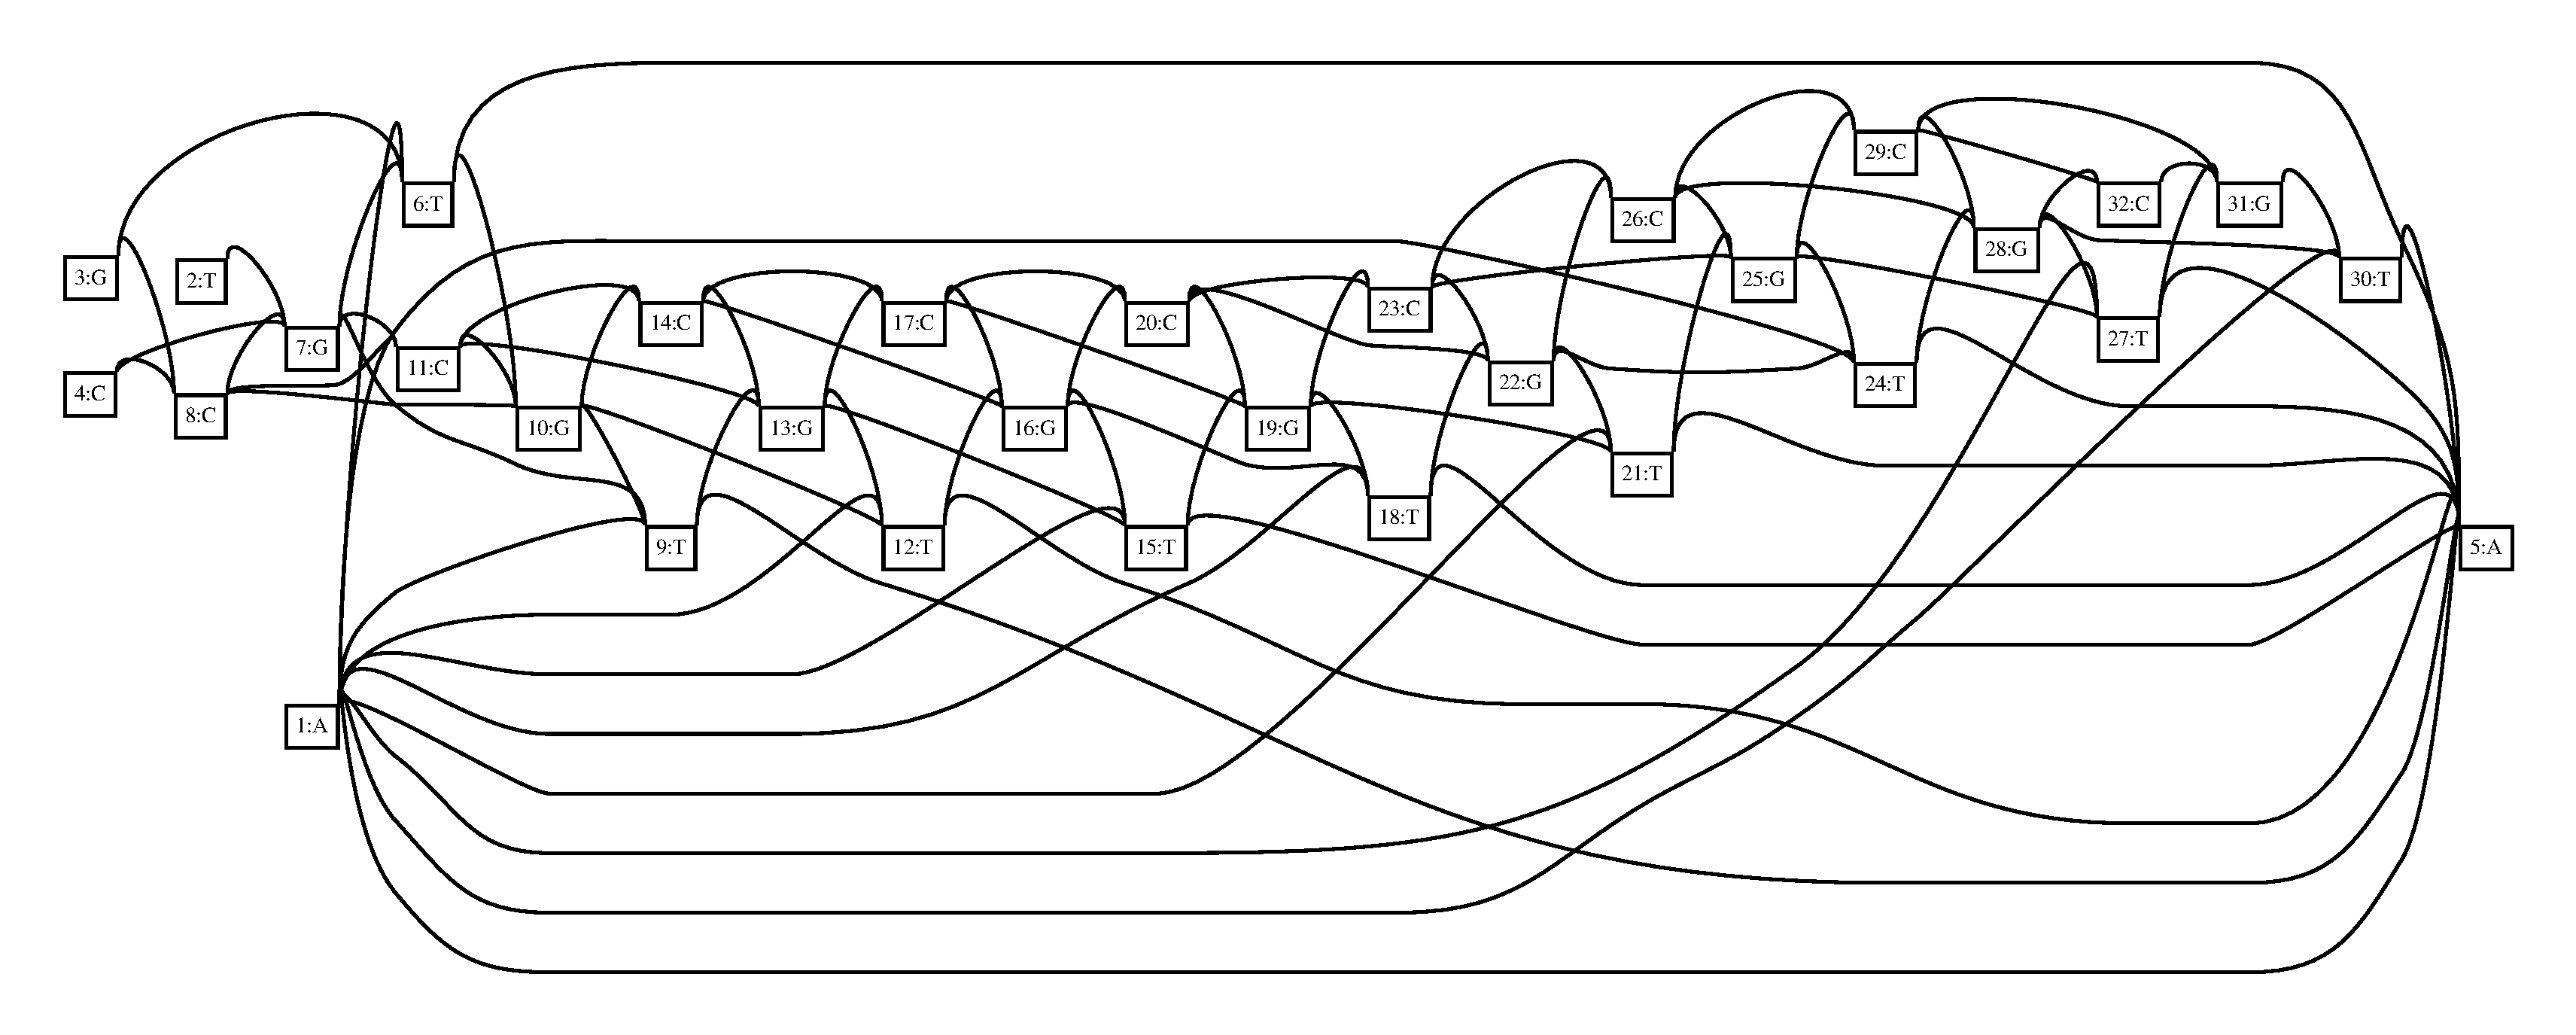
\includegraphics[width=1.0\textwidth]{Chapter2/Figs/loopy_dagify10.pdf}
    \caption{$k=10$} \label{subfig:dagify_k10}
  \end{subfigure}
  \begin{subfigure}[t]{0.49\textwidth}
    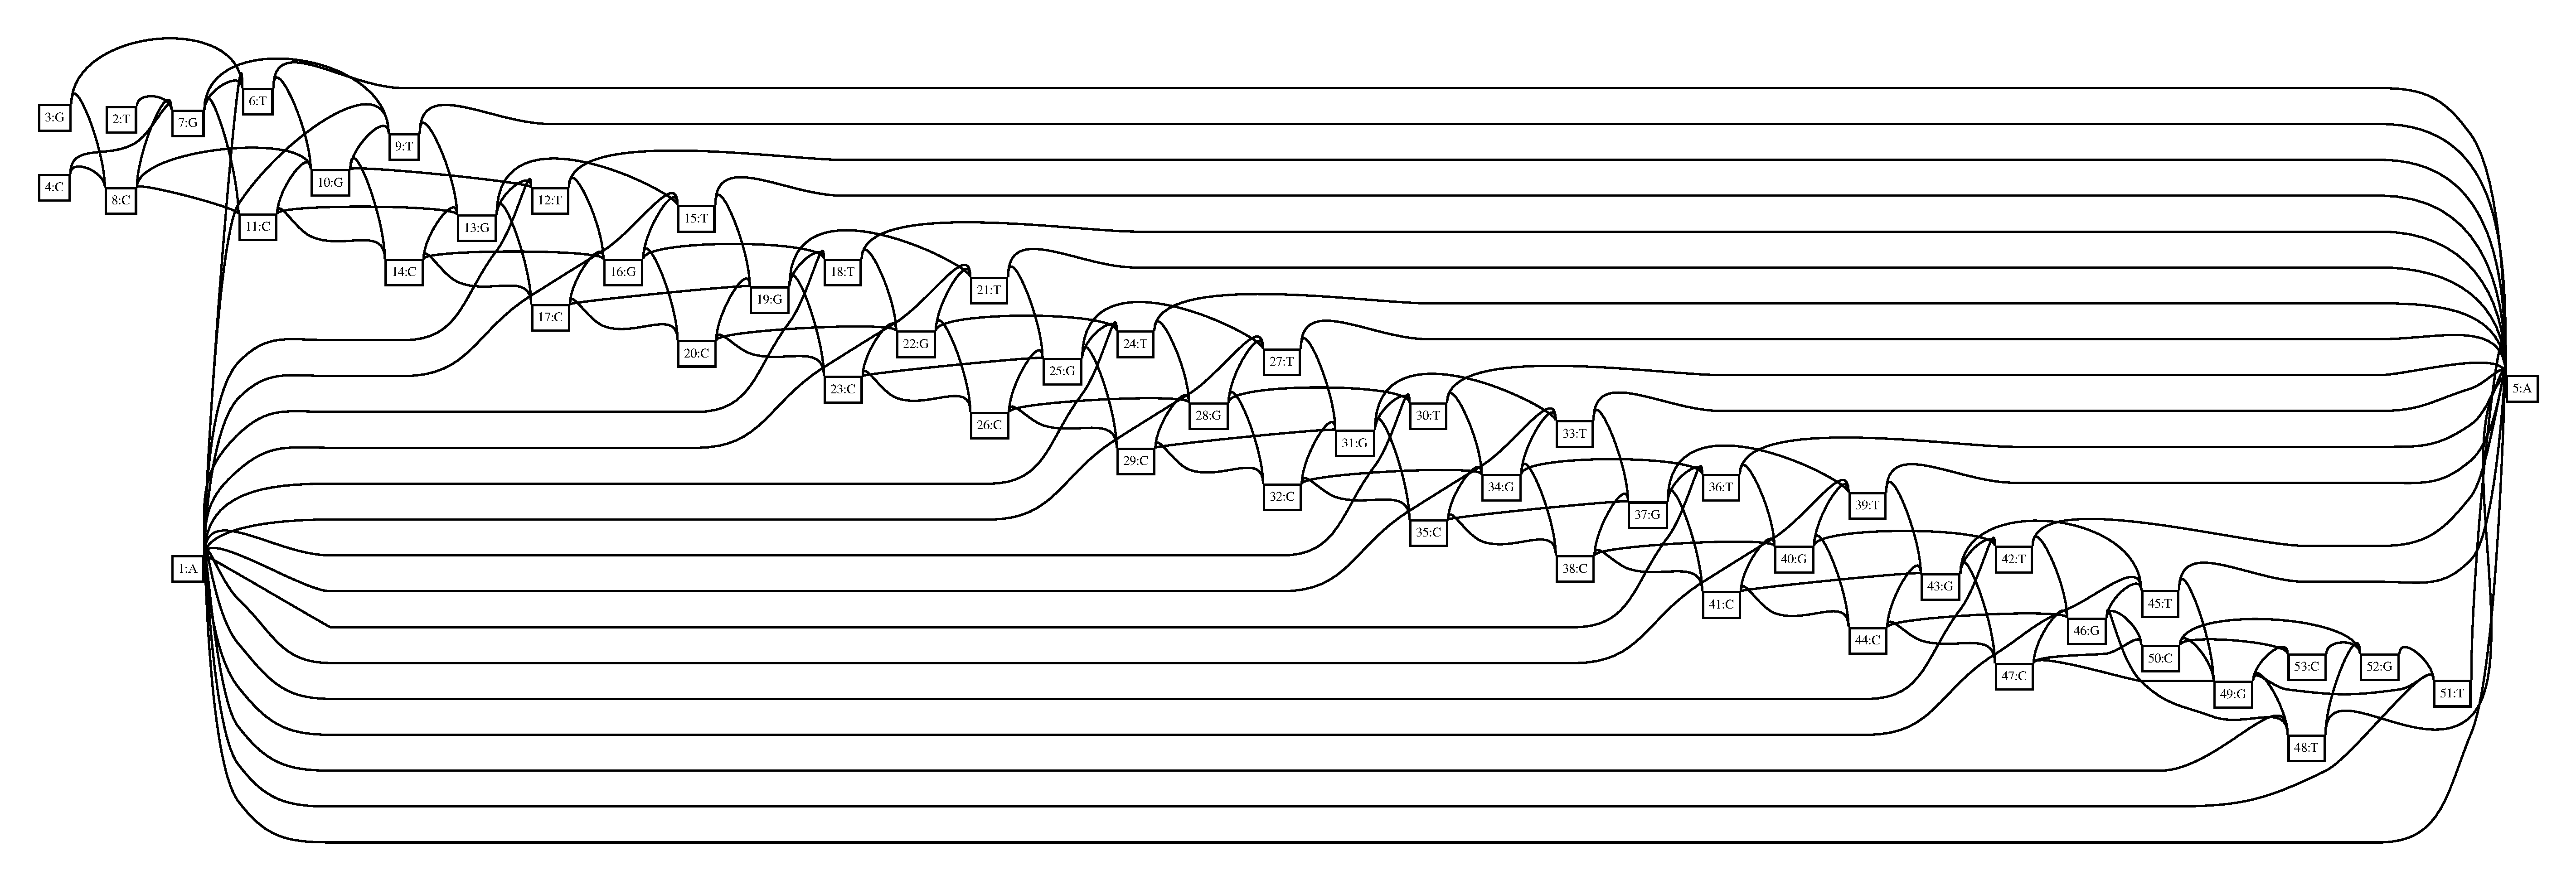
\includegraphics[width=1.0\textwidth]{Chapter2/Figs/loopy_dagify17.pdf}
    \caption{$k=17$} \label{subfig:dagify_k17}
  \end{subfigure}
  \begin{subfigure}[t]{0.49\textwidth}
    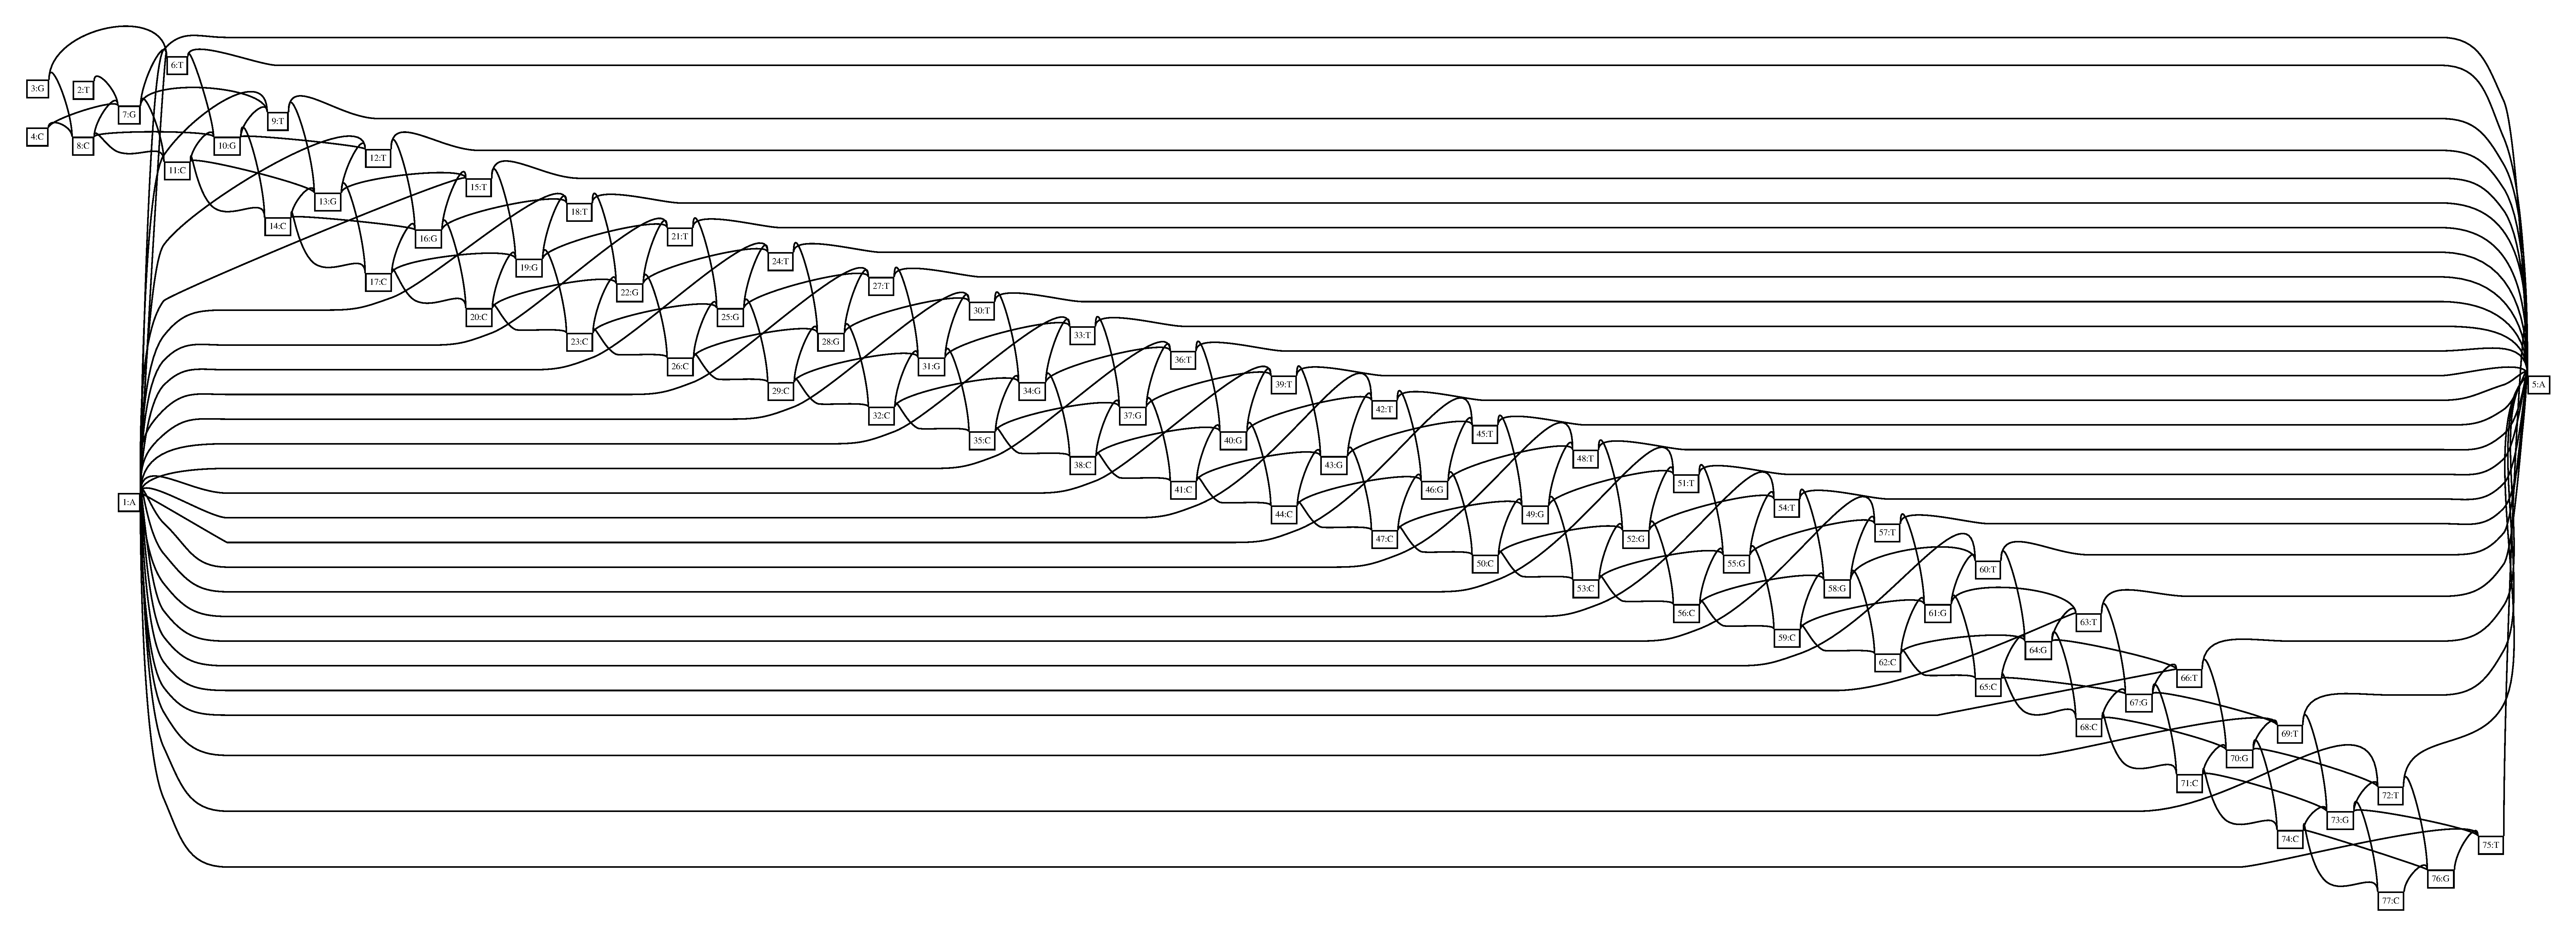
\includegraphics[width=1.0\textwidth]{Chapter2/Figs/loopy_dagify25.pdf}
    \caption{$k=25$} \label{subfig:dagify_k25}
  \end{subfigure}
  \caption[DAGification]{
    DAGification of a small graph, as seen in \ref{subfig:dagify_k0}, with the $k$ unrolling parameter given below each graph.
    In \ref{subfig:dagify_k0} we see a strongly connected component (SCC) of nodes 2, 3, and 4, which is copied in subsequent steps.
    Node ids in subsequent steps are not directly mapped to these original node ids.
    The DAGification algorithm proceeds by greedily breaking the cycles in this component, then copying the component and adding edges from the subsequent copy to the previous for each directed edge within the component until the minimum distance through the unrolled series of SCC copies is at least $k$.
    This minimum distance is tracked using a min-sum DP algorithm that is updated at each copy step by assigning a new minimum length for each node equal to the minimum of the previous minimum length among nodes in the previous SCC copy that it is connected to, plus their sequence label length.
    In panels \ref{subfig:dagify_k10}, \ref{subfig:dagify_k17}, and \ref{subfig:dagify_k25}, we see the unrolled SCC forming a braid in the middle of the rendered graphs, whose length increases with the increase in $k$.
    This algorithm is not optimal, as can be seen by the duplication of paths connecting in and out of the component.
    However, it is linear, and requires only $O(kc)$ time and space, with $c$ representing a constant factor related to the size of the SCCs in the original graph.
  }
\label{fig:dagify}
\end{figure}

\subsection{POA and GSSW}
\label{sec:gssw}
%*2p 2h*

\emph{Graph striped Smith-Waterman} (GSSW)\footnote{\url{https://github.com/vgteam/gssw}} generalizes an implementation \cite{zhao2013ssw} of Farrar's SIMD-accelerated striped Smith Waterman (SSW) algorithm \cite{farrar2007striped} to enable string to graph alignment.
Single-Input Multiple-Data (SIMD) instructions allow vectorized mathematical operations in a single machine instruction, and can be used to greatly speed up algorithms which can be implemented in terms of operations on vectors.

GSSW generalizes all aspects of SSW to operate over sequence directed acyclic graphs, including affine gap penalties, and retains its matrices for traceback\footnote{SSW discards these matrices for performance reasons, instead establishing the traceback later with local banded DP.}.
This is simple to accomplish if the reference is a graph, as the striping of SIMD calculations in SSW across the reference is done by a single character at a time, and thus boundaries between nodes do not split the SIMD embedded variables.
We can generalize SSW to GSSW by extending the recurrence relation that defines the scores in the DP matrices to consider all previous positions on all nodes that connect to the current one.

Given a query $Q$ and a sequence graph $G = (N, E)$ with sequence length $L=\sum_{i}^{|N|} |seq(n_i)|$.
We record the maximum scores of partial alignments between $Q$ and $G$ in the set of matrices ${\cal H} = {\cal H}_1 \ldots {\cal H}_{|N|} :$ each ${\cal H}_i$ is a $|seq(n_i)| \times |Q|$ matrix.
${\cal H}$ thus contains $|Q|\times L$ cells.
When we have completed the scoring phase of alignment each ${\cal H}_{i}[x,y]$ will record the maximum score of an alignment between $Q$ and $G$ ending at $(n_i[x], Q[y])$\footnote{Here I will use brackets $[\ldots]$ to identify the cells in 2-dimensional arrays.}.
To develop our scores, we use a scoring function $score(a, b)$, which in the case of DNA returns the value of a match (typically a positive integer) when $a = b \lor a = N \lor b = N$ and the value of mismatch when $a \neq b$ (typically a negative integer).
We score a gap beginning with $\omega_\textbf{open}$ and a gap extension as $\omega_\textbf{extend}$.
We record the score of a gap along $G$ in matrices ${\cal E} = {\cal E}_1 \ldots {\cal E}_{|N|}$ and a gap along $Q$ in matrices ${\cal F} = {\cal F}_1 \ldots {\cal F}_{|N|}$.

Gaps in $\hat{\cal E}$ extend across the graph, and so we need to consider all the inbound edges when we are at the beginning of a node:

\begin{equation}
  {\cal E}_i[x,y] = \max
  \begin{cases}
    {\cal E}_i[x,y-1] - \omega_\textbf{extend} \\
    {\cal H}_i[x,y-1] - \omega_\textbf{open} \\
    \max_{\forall j : \exists e_{ji} \in E} {\cal E}_j[|n_j|,y-1] - \omega_\textbf{extend} & \text{if } x = 1 \\
    \max_{\forall j : \exists e_{ji} \in E} {\cal H}_j[|n_j|,y-1] - \omega_\textbf{open} & \text{if } x = 1 \\
  \end{cases}
\end{equation}

However, this is not the case for $\hat{\cal F}$, whose data dependencies flow vertically over the query $Q$:

\begin{equation}
  {\cal F}_i[x,y] = \max
  \begin{cases}
    {\cal F}_i[x-1,y] - \omega_\textbf{extend} \\
    {\cal H}_i[x-1,y] - \omega_\textbf{open} \\
  \end{cases}
\end{equation}


The score in $\hat{\cal H}$ combines the affine gap calculations in $\hat{\cal E}$ and $\hat{\cal F}$.
As with $\hat{\cal E}$, we here we also must consider the inbound nodes:

\begin{equation}
  \label{eqn:gssw_h}
  {\cal H}_i[x,y] = \max
  \begin{cases}
    0 \\
    {\cal E}_i[x,y] \\
    {\cal F}_i[x,y] \\
    {\cal H}_i[x-1,y-1] - score(Q[x], n_i[y])\\
    \max_{\forall j : e_{ji} \in E} {\cal H}_j[|n_j|,y-1] - score(Q[x], n_j[y]) & \text{if } x = 1 \\
  \end{cases}
\end{equation}

The values of ${\cal H}_i$, ${\cal E}_i$, and ${\cal F}_i$ are 0 when $x = 0$ or $y = 0$ and node $n_i$ has no inbound edges.
Note that this is the initial condition provided by Gotoh to improve the algorithm of Smith and Waterman.

We fill the matrices using Farrar's SSW algorithm \cite{farrar2007striped}, based on Zhao's implementation \cite{zhao2013ssw}.
By storing the full score matrices we can then trace back from the maximum score in $\hat{\cal H}$ to obtain the optimal alignments under our scoring parameters.
The traceback can be represented as moves in the matrix, or equivalently as the alignment object model described in section \ref{sec:alignments}.

\subsection{Banded global alignment and multipath mapping}
\label{sec:banded_global}

By modifying equation \ref{eqn:gssw_h} so that it is no longer lower-bounded at 0 and changing the traceback so that it goes from beginning to end of query $Q$ and graph $G$, we obtain a ``global'' alignment algorithm with the same properties as Needleman-Wunsch.
To reduce computational costs, we can \emph{band} the algorithm to limit the region of the DP tables which needs to be explored.
This approach, as implemented in {\tt vg} by Jordan Eizenga, forms the basis for multipath mapping, in which alignments are represented probabilistically as DAGs rather than linear series of node traversals and edits.
In multipath mapping, regions between MEMs in a particular cluster are aligned using global alignment.
The use of global alignment ensures that the alignment fully covers the gap between the MEMs.
Multiple traceback allows for alternatives to be included, and each of these may be scored on the basis of both alignment score and haplotype matching score.
His implementation is key to the development of haplotype aware mapping, which is the subject of a paper currently in preparation by myself and collaborators on the {\tt vg} project.
In the case of low-error reads, this limited exploration of the DP problem allows for fast derivation of the optimal alignments, and so the multipath mapper in {\tt vg mpmap} achieves runtime comparable to or exceeding {\tt vg map}.
Multipath mapping concepts also form the basis for alignment surjection, in which an alignment to the graph is projected into the linear reference.

\subsection{X-drop DP}

As our query length $|Q|$ increases, so does the practical complexity of deriving the alignment using POA/GSSW.
We align longer queries against larger graphs, and so we effectively face a quadratic penalty with increasing alignment length, $|Q| \propto |L| \implies$ GSSW is $O(|Q|^2)$.
The most direct solution to this is to use a banded alignment method like banded global alignment, as described in section \ref{sec:banded_global}.
However, this method cannot exploit data parallel operations that allow dramatic speedups on modern processors.

In the course of our work on {\tt vg}, Eizenga and I explored the application of Hajime Suzuki's adaptive banded global alignment (libgaba)\footnote{\url{https://github.com/ocxtal/libgaba}} \cite{suzuki2017acceleration}, which has been used in {\tt minimap2} to greatly improve alignment speed with long single-molecule reads \cite{li2018minimap2}.
In this approach, an antidiagonal band of cells is computed at each step, of a predetermined width designed to fit into the word sizes of SIMD instructions.
The band can move either ``right'' or ``down'' at each step, depending on where the highest score is found.
A termination criterion is given, so that alignment stops when the maximum score falls a given amount.
This is similar to the X-drop parameter used in BLAST to stop alignment extension.
Although it improves performance, it can hurt sensitivity to indels.

Suzki had already implemented a version of alignment over graphs by transforming the graph into a tree through a dynamic unrolling process akin to that described in \ref{sec:DAGify} and aligning to the tree using libgaba\footnote{\url{https://github.com/ocxtal/comb}}.
His implementation supports graph to graph alignment as described in section \ref{sec:translation}, but the exponential expansion of the alignment problem on trees is fundamentally limiting.
Eizenga, Suzuki and I discussed methods to merge the bands together after traversal of unifications in the graph, but we could not establish a safe generic method to merge them.
Furcated bands may only be merged directly if they map to the same query coordinate.
This is unlikely to happen if the different paths in the graph that they have traversed have different lengths or if there are indels in the alignment.

During a biohackathon meeting in Kyoto, Suzuki presented an alternative banding model based on the ``X-drop DP'' algorithm from BLAST.
In this model, the alignment is matrix broken into vertical non-striped windows that tile across the DP matrices over fixed subsequences in the query.
To efficiently resolve the data dependencies between successive steps, a SIMD shuffle operation is applied to the cell values stored in each window.
Forward progression of each window stops when the highest score in the forefront cells drops $X$ below the previously-observed maximum.
This approach thus allows the band to spread as wide as needed to accommodate larger insertions, while being bounded by the $X$-drop parameter.
The result is an approach that is more sensitive than the antidiagonal banded alignment in libgaba, but runs a factor of 2 slower for equivalent band sizes.

\begin{figure}[htbp!] 
\centering    
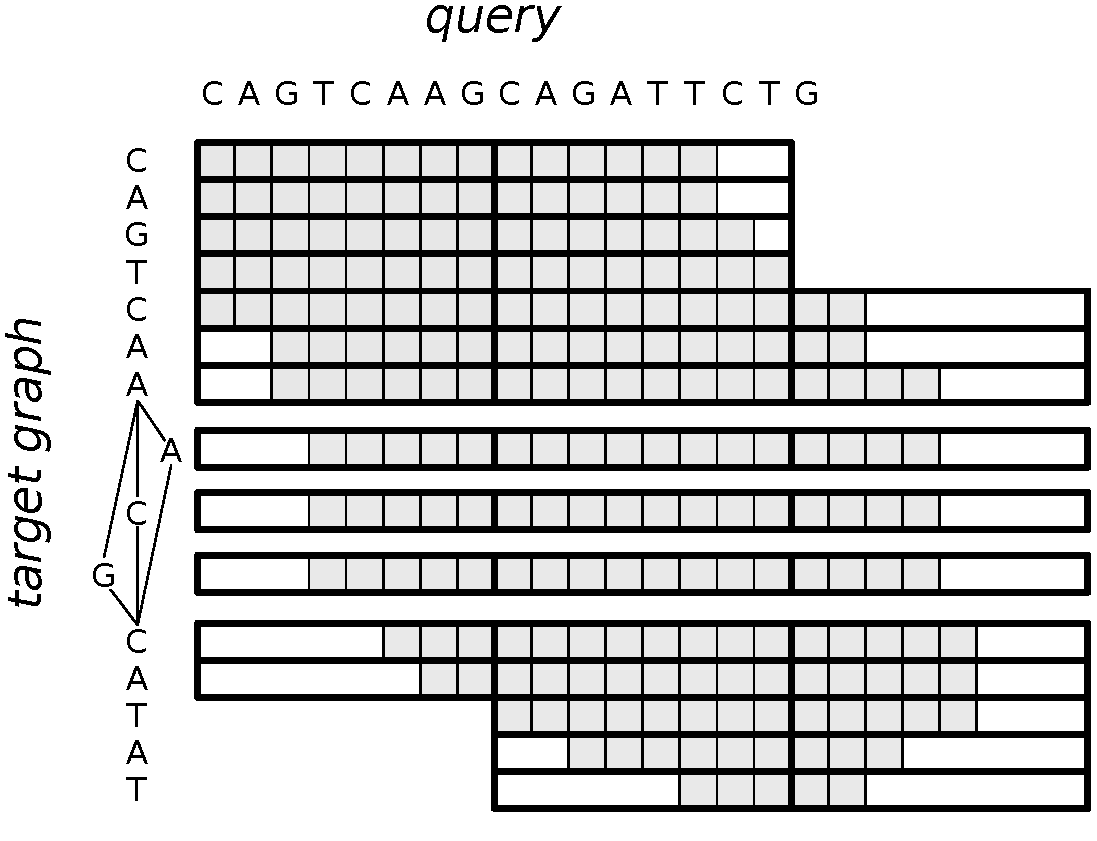
\includegraphics[width=1.0\textwidth]{Chapter2/Figs/xdrop.pdf}
\caption[The \emph{dozeu} X-drop alignment algorithm]{
  Evaluation of the \emph{dozeu} X-drop alignment algorithm for an example graph.
  Gray cells represent the part of the score matrix for which our X-drop parameter would allow evaluation if we were calculating the matrix one cell at a time.
  8-cell wide black rectangles that contain the full set of gray cells represent the region of the score matrix for which we calculate scores when using a SIMD-based accelerated version of the algorithm.
  Traceback and per-cell scores are not shown.
  This figure is meant to illustrate the adaptive banding property of the X-drop algorithm and how that can be used in a SIMD-based acceleration of the algorithm.
  Adapted with permission from \url{https://github.com/ocxtal/dozeu}.
}
\label{fig:xdrop}
\end{figure}

I have since worked with Suzuki to integrate his implementation of this algorithm \emph{dozeu}\footnote{\url{https://github.com/ocxtal/dozeu}} into {\tt vg}.
Due to difficulties in handling paired end rescue, the approach is not yet performing as well as GSSW for {\tt vg map}.
This remains a work in progress, but is a promising approach to enable the direct alignment of long sequences against the graph.
It is orthogonal to the ``chunked'' alignment approach, and in principle, they can be applied together to build a SV-aware, chunked and banded alignment process.
Future work in this direction may yield a new VG alignment algorithm, but this lies outside the scope of this thesis.

\subsection{Chunked alignment}
%*1p 1h*
\label{sec:chunked_alignment}

For long reads, where in the worst case the local dynamic programming can become prohibitively expensive, we break the reads into ``bands'' of a fixed width $w$ (default 256 base pairs) with overlap between successive bands of $w/8$.
Chunking the alignment process allows us to directly detect complex structural variation within our alignment, and provides a kind of split read alignment model for {\tt vg}.
We align these bands independently, trim the overlaps from the alignments, and build an alignment DAG model $G_\textsc{AlignChain} = (N, E)$ similar to that built for MEM chaining (as in \ref{sec:collinear_chaining}).
The only significant difference between these two models is that in $G_\textsc{AlignChain}$, we consider sub alignments as nodes in the model rather than MEMs.

In this model we put weights on transitions between alignments that relate to the estimated distance between the alignments in the graph versus their distance in the read, with the objective of making long co-linear chains be the highest-scoring walks through the chaining model.
We take the max-sum path through the model to be the best alignment.
Then, to obtain multiple alignments, we mask out this path, re-score, and take the next max-sum path to get the 2nd-, 3rd-, and ultimately $N$th-best alignment.

After they have been extracted from the model, alignments are ``patched'' using local alignment of unaligned regions anchored in the graph near the end of previous mapped regions, so that sub-alignments which may have been misaligned due to repeats may be locally aligned correctly.
This model allows {\tt vg} to map noisy reads of arbitrary length, and is used as a core component in the long read progressive assembler {\tt vg msga}.

Although the development of $G_\textsc{AlignChain}$ is very similar to $G_\textsc{MemChain}$, a number of important differences distinguish the two models.
I will fully describe the chunked alignment chaining model here so that it may stand apart from the MEM chaining model.

\begin{figure}[htbp!]
\centering
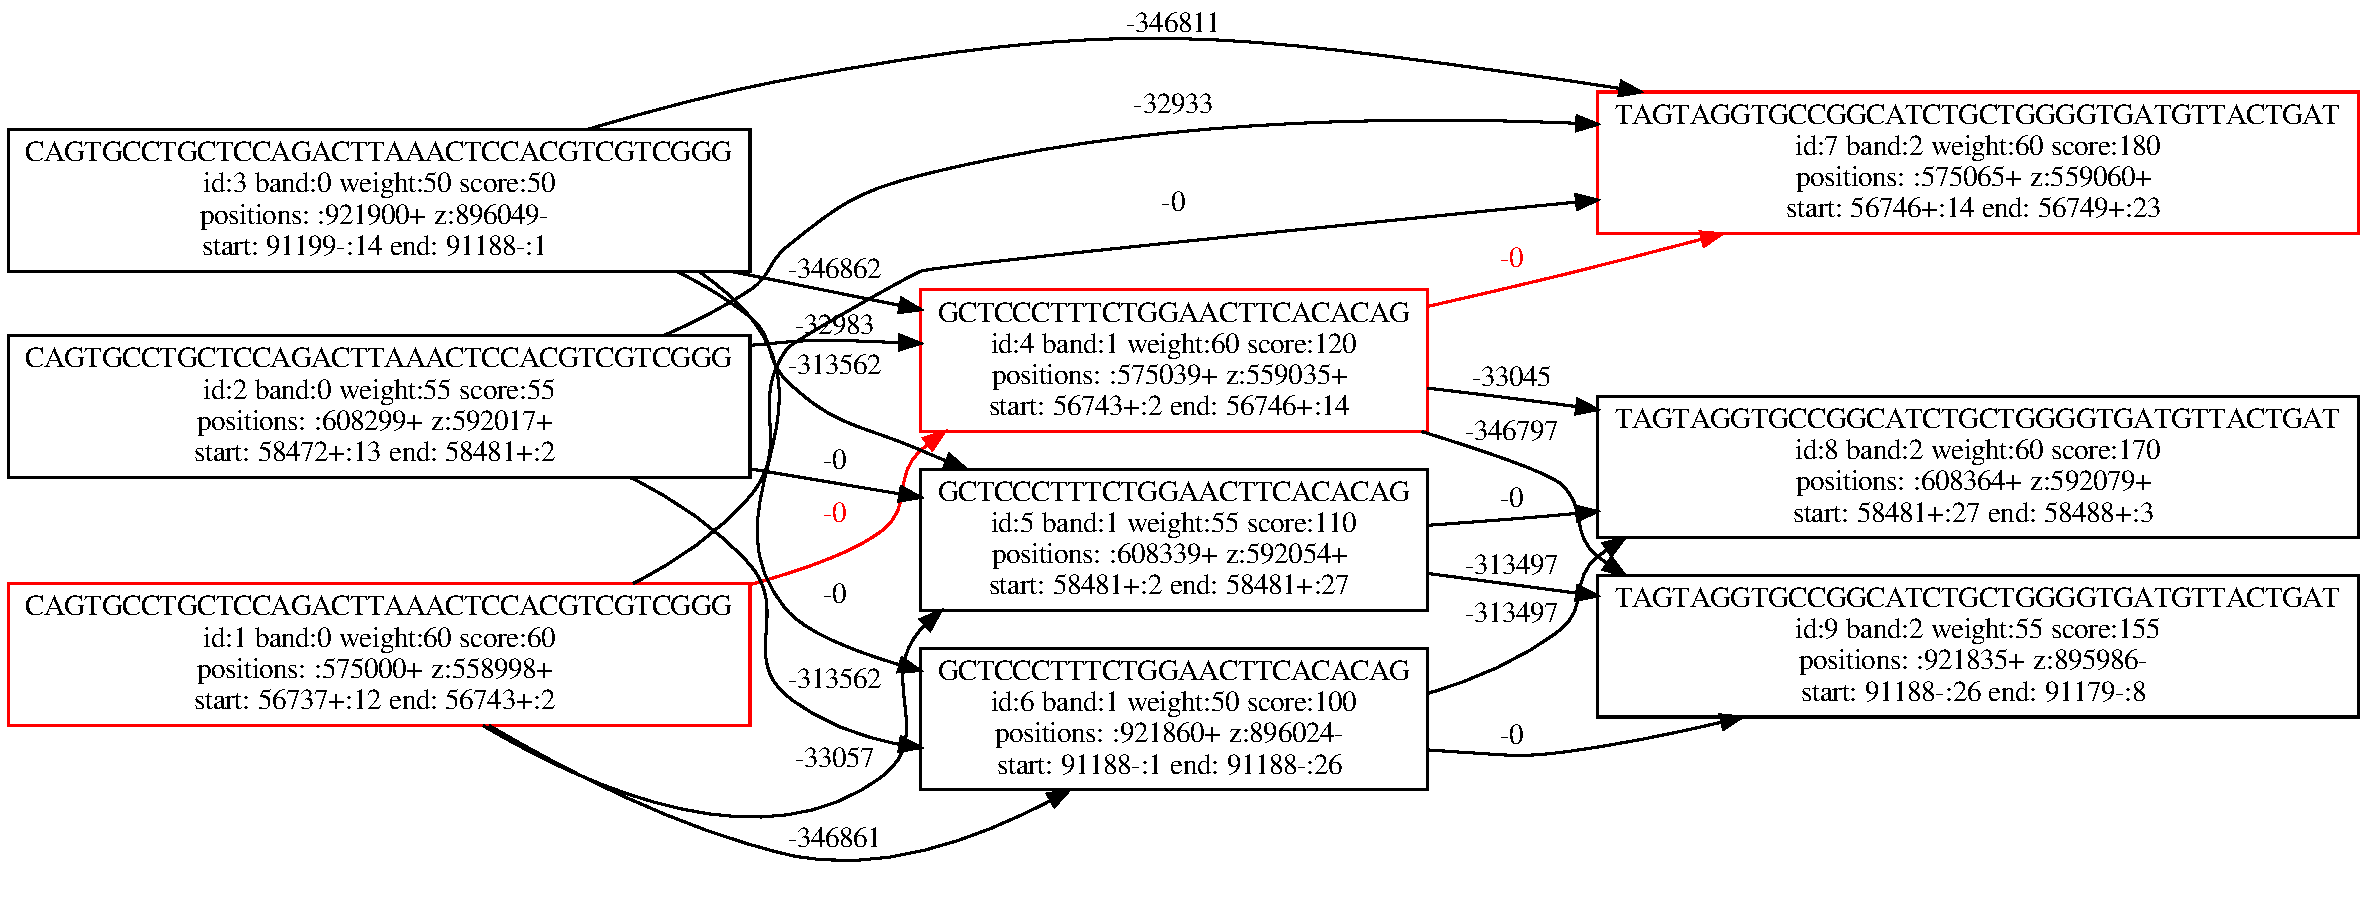
\includegraphics[width=1.0\textwidth]{Chapter2/Figs/alignchain_dag.pdf}
\caption[The Alignment Chain Model]{
  The first evaluation of the alignment chain model for a set of alignment bands derived from a simulated query mapped against a test 1Mbp 1000GP graph included in the {\tt vg} repository, using {\tt vg map} parameters {\tt -w 50 -O 25 -J 2} to simplify the model for exposition.
  Each node refers to a single mapping of an alignment band, its sequence, weight, its band index among bands taken from the original query, a node id in the graph, and the score derived from the first pass of the max-sum algorithm.
  %Each of the three bands has been aligned to three locations in the reference graph, resulting in three columns of nodes, with each column corresponding to a given band.
  Edges are labeled with their derived weight ${\cal W}_{e_{ij}}$, which can be seen to be 0 for edges connecting bands whose end and start positions directly connect.
  The maximum scoring chain is shown in red, and corresponds to the correct mapping location of the simulated query.
}
\label{fig:alignmentchain_model}
\end{figure}


As each subalignment is part of the full alignment that we'll derive by finding the max-sum path through the model, we apply use the alignment score to set the initial weight for the node:

\begin{equation}
  {\cal W}_{n_i} = alignment\_score(n_i)
\end{equation}

Each alignment node $n_i$ has a set of graph start and end positions $graph\_start\_pos(n_i) = \{ b_1 \ldots b_m \}$, $graph\_end\_pos(n_i) = \{ b_1 \ldots b_m \}$.
We use these to provide weights for the edges in the alignment chain model.
Edges $e_{ij}$ in $G_\textsc{AlignChain}$ represent possible transitions between sub-alignments, and are weighted (${\cal W}_{e_{ij}}$) by the minimum estimated distance between the given graph positions for each alignment end, times the gap open and extension costs.
The alignment bands overlap during the alignment of each sub-alignment, but at the point when we establish the model, we have trimmed the overlaps between successive sub-alignments and re-calculated the alignment score, so we do not need to consider them here.
Unlike the MEM chaining model, which is driven entirely by approximate distances, when we obtain an estimated distance less than the length of the alignment chunk, we walk the graph using a depth first search in order to obtain a precise minimum value for the distance.

\begin{equation}
  dist_{e_{ij}} = \min_{dist(b,d)} \forall b \in graph\_end\_pos(n_i), \forall d \in graph\_start\_pos(n_j)
\end{equation}

The chunked alignment model allows us to align through inversions, which we score using a basic heuristic that they are twice as costly as a gap of the same length as the inverted sequence.
The inversion distance estimate walks forward from the positions in $n_j$ and seeks $n_i$.
In the case of a non-inversion, the resulting estimate will be $\infty$, as $n_i$ will never be reached by walking forward from $n_j$.

\begin{equation}
  dist\_inv_{e_{ij}} = dist_{e_{ji}}
\end{equation}

\begin{equation}
  {\cal W}_{e_{ij}} = \max
  \begin{cases}
    \omega_\textbf{extend} dist_{e_{ij}} + \omega_\textbf{open} [dist_{e_{ij}} \ne 0] \\
    2 \times \left( \omega_\textbf{extend} dist\_inv_{e_{ij}} + \omega_\textbf{open} [dist\_inv_{e_{ij}} \ne 0] \right)
  \end{cases}
\end{equation}

These node and edge weights relate to the final alignment score that we would expect should we concatenate a particular series of sub-alignments.
%We expect a positive score due to an exact match, so we apply a positive weight to each node as it represents a MEM.
%Transtions between sub-alignments may encode gaps or mismatches.
We cannot precisely estimate the final score of the read without the final patching step, but we can use our position index and the function $dist(b,d)$ to estimate gap lengths.
We take the score of a concatenated alignment ${\cal P} = n_i \ldots n_j$ in the model to be:

\begin{equation}
  {\cal S}_{\cal P} = \sum_{i = 0}^{|{\cal P}|-2} {\cal W}_{{\cal P}[i]} + {\cal W}_{e_{{\cal P}[i]{\cal P}[i+1]}}
\end{equation}

Given this definition, we expect the maximum sum walk ${\cal P}_\textsc{max} = n_i \ldots n_j$ through the graph to be likely to yield the series of sub-alignments and graph positions involved in the maximum scoring alignment we would obtain should we have aligned the entire query in one step.
This concatenated alignment is approximate due to the incompleteness of our score estimate and the fact that our alignment set is not guaranteed to capture the optimal alignment due to the arbitrariness of the banding pattern that we have applied.
Incompleteness due to our partitioning of the alignment problem means that to obtain a precise score we must locally realign unaligned portions of the concatenated alignment.
This alignment patching process resolves problems that can occur due to induced soft clips, fully unaligned bands, or structural variations such as inversions or small CNVs that frustrate the complete alignment of a particular band.

As with the MEM chaining model, we derive partial alignments from $G_\textsc{AlignmentChain}$ by applying a standard max-sum dynamic programming algorithm to derive the maximum possible final alignment score at each node, and then, by working from the maximum scoring node, derive the maximum scoring path through the graph.
The score for each node ${\cal S}_{n_i}$, combines the sum of own weight, the maximum score of any previous node it is connected to, and the weight of the edge connecting the maximum scoring inbound node and the current node:

\begin{equation}
  {\cal S}_{n_i} = {\cal W}_{n_i} + \max_{\forall e_{ji} \in E} \left( {\cal W}_{e_{ji}} + {\cal S}_{n_j} \right)
\end{equation}

To allow traceback of the maximum scoring path, we record the maximum inbound node for each node.

\begin{equation}
  {\cal T}_{n_i} = \operatorname*{argmax}_{n_j} \left( {\cal W}_{e_{ji}} + {\cal S}_{n_j} \right)
\end{equation}

At the end of the scoring phase, we find the highest scoring node.

\begin{equation}
  n_{max} = \max_{\forall n_i \in N} {\cal S}_{n_i}
\end{equation}

Walking back through the series of recorded traceback pointers yields the maximum scoring concatenated alignment under the alignment scoring and transition weight model we've applied.
We define the series of nodes in the max-sum path by $n_{max-i-1} = {\cal T}_{n_{max-i}}$.
The resulting path is expressed in reverse order relative to our traceback.

\begin{equation}
  {\cal P}_\textsc{max} = n_{max-|{\cal P}_\textsc{max}|} \dots n_{max-1}, n_{max}
\end{equation}



\subsection{Alignment surjection}
\label{sec:surjection}

Alignments to graphs that include linear reference sequences as paths can be transformed into alignments against those paths.
Alignment \emph{surjection} projects alignments to the full graph \emph{onto} the subgraph defined by a given set of paths in the graph.
This transformation is used to project graph based alignments onto the linear reference, and is of great utility in the application of {\tt vg} in resequencing based analyses, where it supports a lossy translation between {\tt vg}'s native GAM format and BAM.

In surjection, portions of the alignment that already map to the path specific graph subset are left unchanged.
However, regions of the original alignment to parts of the graph that are not in the selected path subset are mapped onto the nearest suitable node, with additional edits to specify the differences between the alignment and the graph subset defined by the target paths.
To produce a meaningful alignment, surjection requires that the alignment path matches the reference path for some portion of its length.
Otherwise, the resulting alignment would be empty, or unaligned.

The name ``surjection'' is meant to be illustrative, and is not mathematically precise in the sense that it only applies to the alignments in terms of the node space of their paths.
When we consider only the set of nodes that are traversed by a given alignment and its surjection, it is given that the function is surjective, as the domain of the function is the full graph, while the codomain is the subset defined by a given set of paths, with each node corresponding to one or more nodes in the original graph.
(For instance, a mapping to a non-reference allele would be projected onto the nearest neighboring node in a reference path.)
This surjective property would be violated in the case of a graph that only consisted of nodes in the paths that we are projecting our alignments into, as in this case the projection would bijective or the identity.

However, it is not clear that projecting the alignments into a graph subset defined by a given set of paths is surjective when we consider the full alignment data model.
Information about the original alignment sequence is fully retained in the node mappings of the surjected alignment path, and this can be seen as violating the surjective property of the transformation.

The simplest surjection technique extracts the reference path region matching an alignment and realigns the read against it.
Doing so without global alignment will often result in soft clipping, such as where non-reference alleles in the graph have allowed full length alignment.
This can be resolved to some extent by applying global alignment of the alignment query sequence against the reference.
But a more rigorous approach rebuilds the alignment in parts.
For each piece that is not aligned to the reference, we extract the intervening reference sequence and align only the subset of the query that is no longer matching to this region.
A kind of anchored semi-global alignment may be used on the ends of the reads, where the opposite reference-matching end is not defined.
The resulting alignment may easily be expressed in the BAM format and thus be used by standard downstream variant calling and analysis methods.

\subsection{Base quality adjusted alignment}
%*2p 2h*

Base qualities are typically reported on the Phred scale so that the probability of error for a given quality $Q$ is $\epsilon = 10^{-Q/10}$. Assuming no bias in which bases are mistaken for each other, this defines a posterior distribution over bases $b$ for a base call $x$.

\begin{align}
    P(b|x, \epsilon) = \begin{cases}
        1 - \epsilon & b = x \\
        \frac{1}{3} \epsilon & b \neq x
    \end{cases}
\end{align}

We use this distribution to derive an adjusted score function. Normally, the match score for two bases is defined as the logarithm of the likelihood ratio between seeing two bases $x$ and $y$ aligned and seeing them occur at random according to their background frequencies. 

\begin{align}
    s_{x,y} &= \log\left(\frac{p_{x,y}}{q_y q_x} \right) \label{eqn:base_score}
\end{align}

Next we marginalize over bases from the posterior distribution to obtain a quality adjusted match score.

\begin{align}
    \tilde s_{x,y}(\epsilon) &= \log\left(\frac{(1 - \epsilon)p_{x,y} + \frac{\epsilon}{3}\sum_{b \neq x}p_{b, y}}{q_y\left((1 - \epsilon)q_x + \frac{\epsilon}{3}\sum_{b \neq x}q_b \right)} \right)
\end{align}

{\tt vg} works backwards from integer scoring functions to the probabilistic alignment parameters in this equation. After doing so, the match scores are given by

\begin{align}
    \tilde s_{x,y}(\epsilon) &= \frac{1}{\lambda} \log\left(\frac{(1 - \epsilon)q_x q_y e^{\lambda s_{x,y}} + \frac{\epsilon}{3}\sum_{b \neq x}q_b q_y e^{\lambda s_{b,y}}}{q_y\left((1 - \epsilon)q_x + \frac{\epsilon}{3}\sum_{b \neq x}q_b \right)} \right).
\end{align}

Here, $\lambda$ is a scale factor that can be computed from the scoring parameters, and the background frequencies $q_x$ are estimated by their frequency in the reference graph. Since base quality scores are already discretized, the adjusted scores can be precomputed and cached for all reasonable values of $\epsilon$. 

\subsection{Mapping qualities}
\label{sec:mapping_quality}

The algorithm for mapping qualities in {\tt vg} is also motivated by a probabilistic interpretation of alignment scores.
The score of an alignment $A$ of two sequences $X$ and $Y$ is the sum of scores given in equation \ref{eqn:base_score}.
This makes it a logarithm of a joint likelihood ratio across bases, where the bases are assumed independent (a more complete justification including gap penalties involves a hidden Markov model, but it can be shown to approximate this formula).
We denote this score $S(A|X,Y)$.
Thus, assuming a uniform prior over alignments, we can use Bayes' Rule to motivate a formula for the Phred scaled quality of the optimal alignment, $\hat A$.

\begin{align}
\begin{split}
    Q(\hat A|X,Y) &= -10\log_{10}(1 - P(\hat A|X,Y)) \\
    &= -10 \log_{10}\left(1 - \frac{P(X,Y|\hat A)}{\sum_{A}P(X,Y|A)} \right) \\
    &= -10 \log_{10}\left(1 - \frac{e^{\lambda S(\hat A|X,Y)}}{\sum_{A}e^{\lambda S(A|X,Y)}} \right) \label{basicqualityscore}
\end{split}
\end{align}

Using the close approximation of the \emph{LogSumExp} function by element-wise maximum, there is a fast approximation to this formula that does not involve transcendental functions.

\begin{align}
    Q(\hat A|X,Y) &\approx \frac{10\lambda}{\log 10}\left( S(\hat A | X,Y) - \max_{A \neq \hat A}S(A| X,Y)\right)
\end{align}

In practice, we do not compare the optimal alignment to all possible alignments, but to the optimal alignments from other seeds. Thus, the mapping quality indicates the confidence that we have aligned the read to approximately the correct part of the graph rather than that the fine-grained alignment in that part of the graph is correct. Since this formula is based on alignment scores, it can incorporate base quality information through the base quality adjusted alignment scores.


\section{Visualization}

Visualization helps enormously to understand variation graphs and algorithms on them.
While text-mode renderings are sufficient for evaluating results in resequencing against the linear reference, they are simply impractical when the reference is a graph.
A set of dotplots can allow us to understand the relationship between many paths embedded in a graph.
But this scales quadratically with the number of embedded paths and quickly becomes impossible to interpret.
The alternative is to render graphs visually using a coherent set of visual motifs.

Here I describe several such techniques designed specifically for variation graphs.
The simplest leverage standard utilities for graph drawing, and the most performant of these are hierarchical models that benefit from linear ordering which is often available in reference-ordered variation graphs.
Force-directed layouts techniques developed for assembly graph interpretation allow us to interrogate larger-scale graphs.
While it may be topologically complex, any graph is composed of sets which can be ordered linearly.
By exploiting a linear sort of the graph I provide a linear-time layout algorithm that will scale to arbitrary data scales, allowing the visualization of both paths and read coverage against any graph.

\subsection{Hierarchical layout}
%*0.5p 0.5h*

To develop a visualization method quickly, I relied most heavily on the four-phase hierarchical graph layout algorithm {\tt dot} \cite{gansner1993technique} that is part of the Graphviz package \cite{gansner2000open,ellson2001graphviz}.
This approach tries to generate a layout in which hierarchical structures in the graph are exposed, visual anomalies such as edge crossings and sharp edge bends are avoided, edges are short, and the layout is overall balanced or symmetric.
It first uses a partial sort on the graph to derive a rank for each node.
This aspect of the algorithm means it is best suited for DAGs.
Then the unordered regions of the partially sorted graph are ordered to reduce edge crossings.
Finally, the actual layout is derived and splines are drawn to show edges.
The output of {\tt dot} as well as other tools in Graphviz is a vector graphic, so the resulting renderings may be viewed in a number of ways.

To generate a visualization that captures the structure of the variation graph, I transform the graph into a visualization oriented structure in which the graph paths are rendered as nodes and edges.
The layout is then driven entirely by the chosen algorithm in Graphviz, which is typically {\tt dot}.
This approach allows us to view rather large chunks of graphs, up to tens of kilobases, provided the graph is partially orderable.

The set of nodes may be rendered as boxes labeled by $id(n_i)$ and $seq(n_i)$.
Edges have four types, and to indicate these we use the top and bottom of the node boxes.
The top left corner of each node $n_i$ receives incoming edges $e_{ji} \forall j : e_{ji} \in E$.
While the bottom right corner of each node box represents edges arriving at $\overline{n_i}$ and thus $e_{j\overline{i}} \forall j : e_{j\overline{i}} \in E$.
Similarly, the top right corner of each node box represents edges leaving $n_i$, and we add an edge for each $e_{ij} \forall j : e_{ij} \in E$.
Finally, the bottom left corner represents the ``end'' of the reverse complement of the node $\overline{n_i}$, and, so we add edges for $e_{\overline{i}j} \forall j : e_{\overline{i}j} \in E$.
As each edge implies its own reverse complement, we tend to replace edges $e_{\overline{ij}}$ with $e_{ji}$, and this is done both in normalization as in Graphviz based rendering.

Paths are not naturally supported in the Graphviz data model, and must be added as subgraphs with a different rendering style to identify them.
In order to achieve a visually meaningful layout, these subgraphs must be also anchored appropriately into the graph.
For each path, I hash the path name $name(p_i)$ into a set of colors and Unicode emoji, yielding $8 \times 766 = 6128$ possible color/symbol combinations.
This generates a symbol for each path that is unlikely to collide with another given the typical application rendering a graph with tens of embedded paths.
The hashing process also ensures the same rendering is returned as long as the same path names are given.
For each mapping $m_i\ldots m_{|p_j|} \in p_j$ I add invisible edges to the graph that link the mapping to the particular node it maps to as well as a visible edge in the path color from $m_{i-1} \to m_i$ when $i > 1$ and from $m_i \to m_{i+1}$ when $i < |p_j|$.
A hint is given to {\tt dot} to force the rank of each mapping to be the same as the node it maps to.
Otherwise, the invisible edges encourage {\tt dot} to render the path mappings close to the node they refer to.
The resulting layout tends to look like a kind of multiple alignment matrix, as can be seen in figure \ref{fig:vg_view_dot}.

\begin{figure}[htbp!] 
\centering    
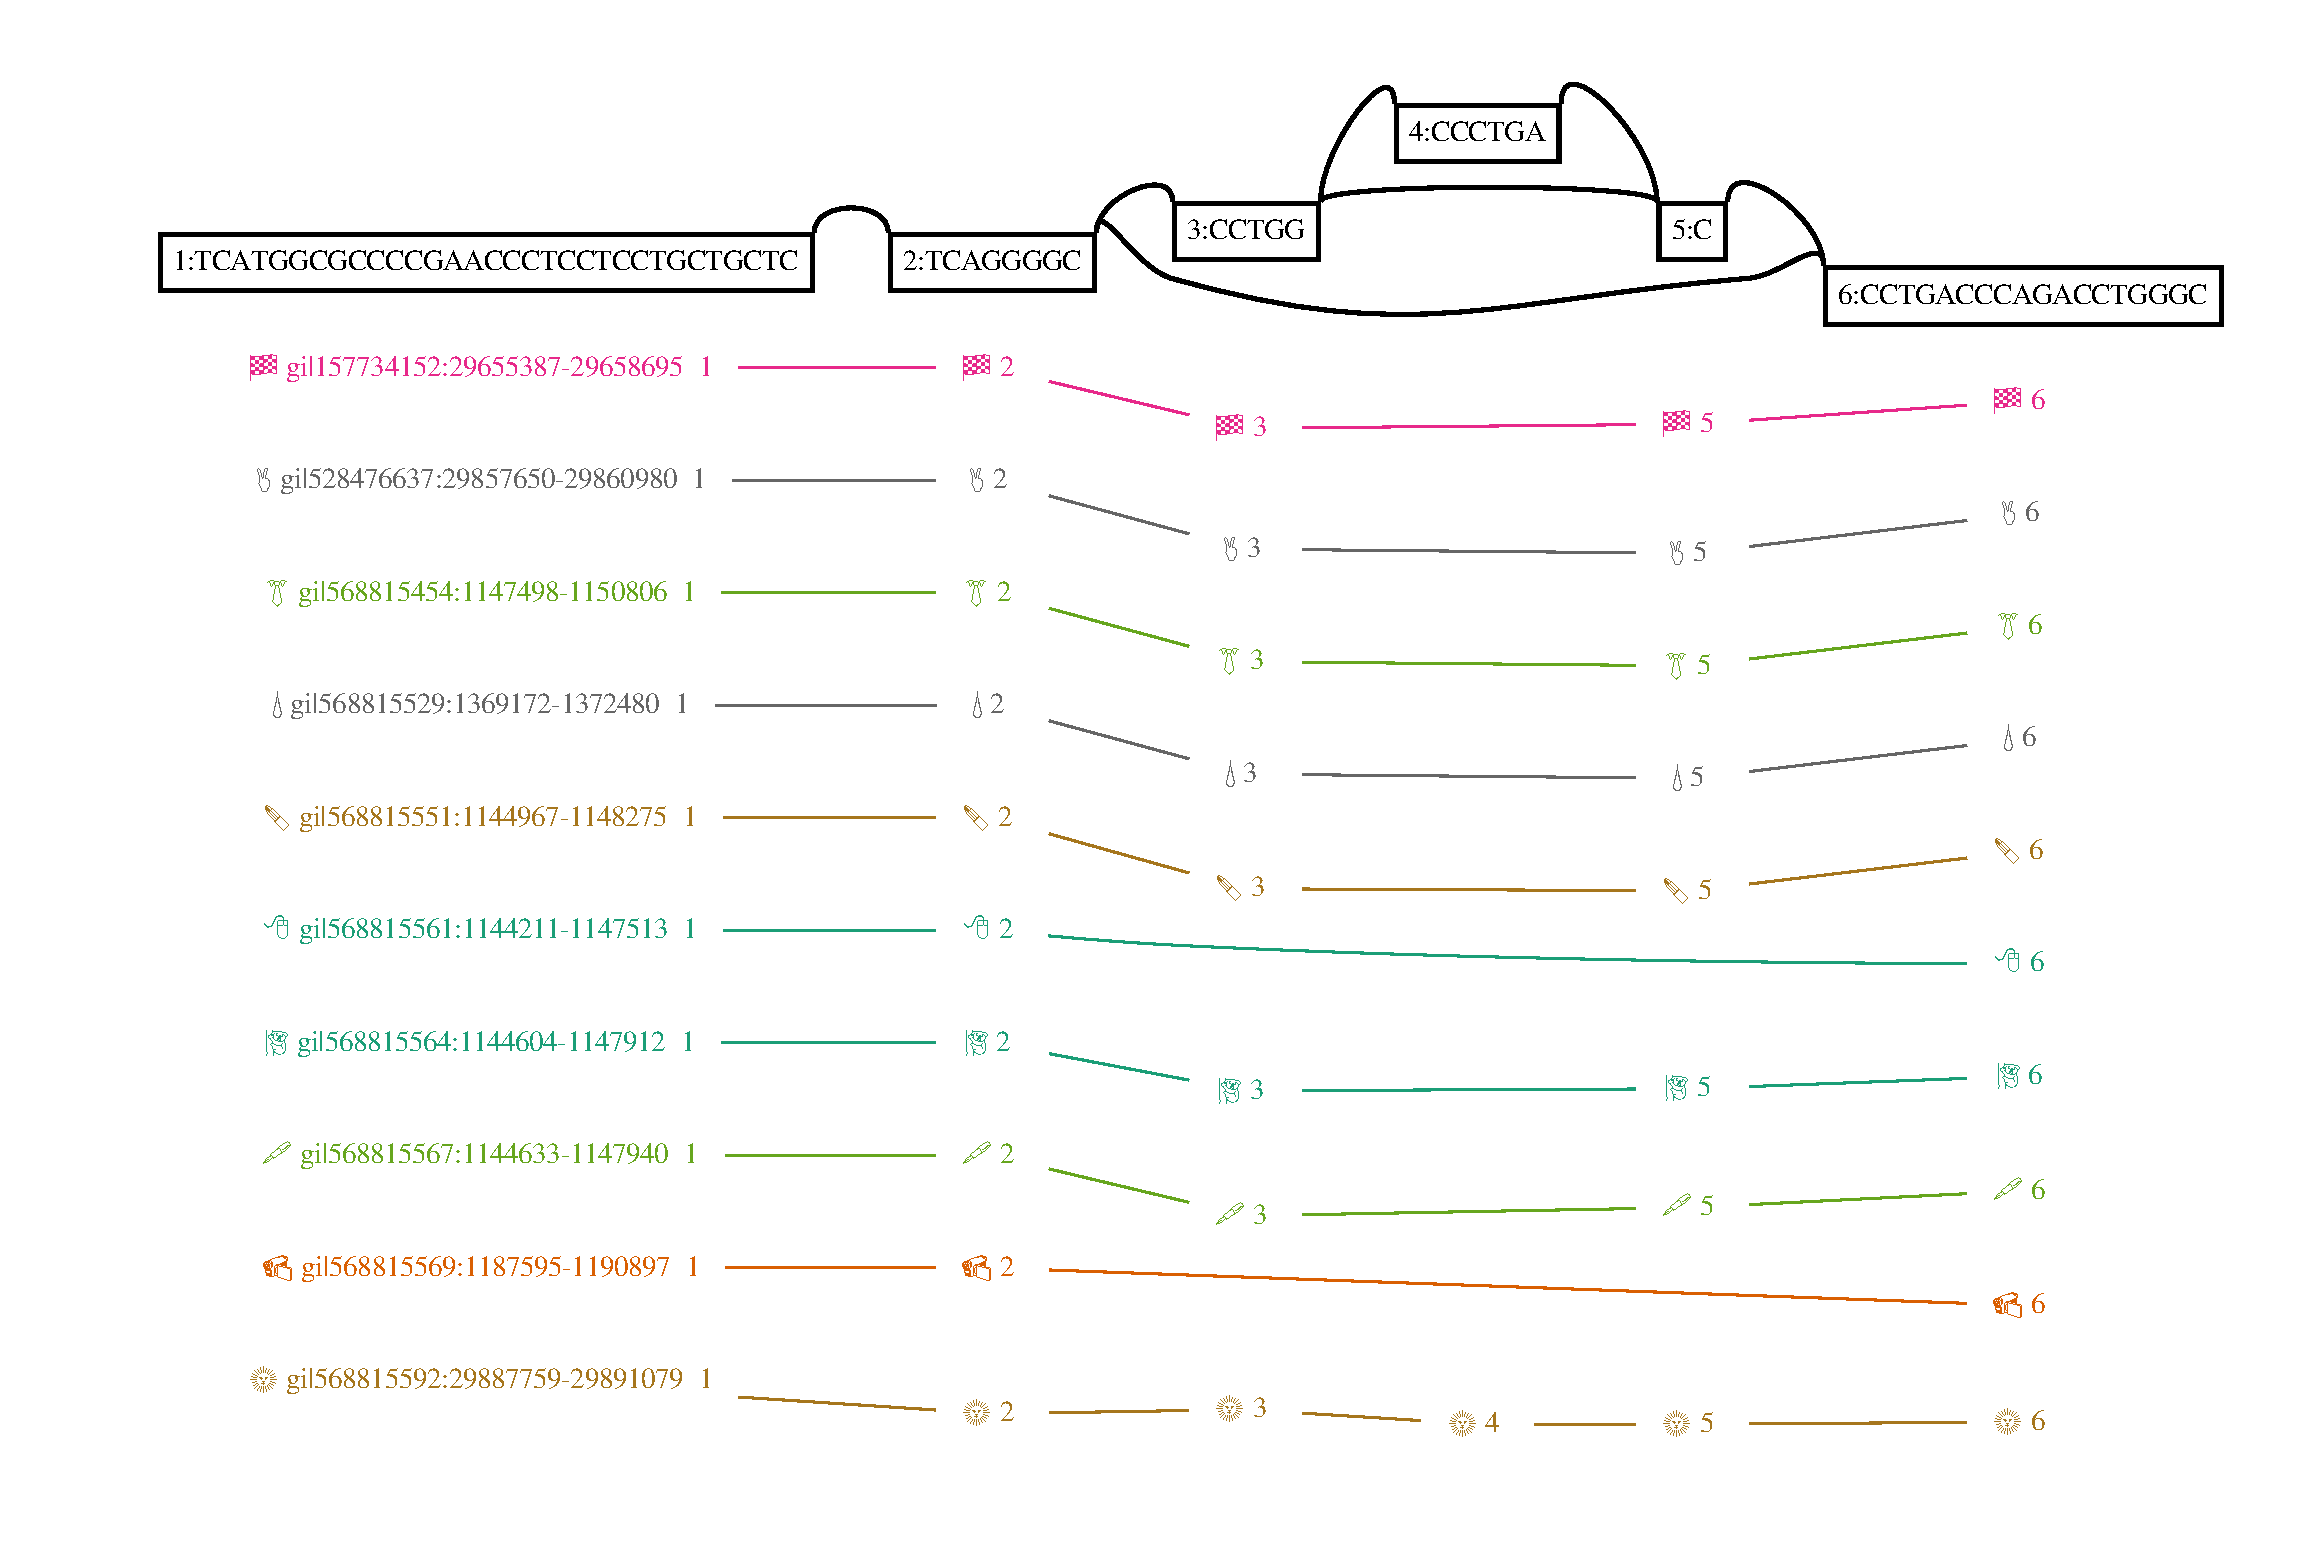
\includegraphics[width=1.0\textwidth]{Chapter2/Figs/vg_view_dp_H-3136_dot.pdf}
\caption[Hierarchical visualization with Graphviz's {\tt dot}]{The beginning of a variation graph built by progressive assembly of the GRCh38 haplotypes in HLA gene H-3136 visualized using {\tt dot}.
  The graph topology of nodes and edges is represented above, with node ids and sequences labeled the rectangular nodes, and edges connecting the upper corners of nodes representing the edge topology relative to the forward strand of the graph.
  Below, paths in the graph are represented in a matrix-like format, with each mapping in the path represented by a node id and a colored emoji, and subsequent steps connected by a colored line.
  The emoji/color combination is determined by a hash function applied to the path name.
  A hidden edge connecting each path mapping step and the corresponding node in the graph topology is used to force the rendering to place them at the same horizontal position, increasingly legibility.
}
\label{fig:vg_view_dot}
\end{figure}

\subsection{Force directed models}
%*1p 1.5h*

Not all graphs yield easily to hierarchical layout algorithms.
Graphviz also includes a force-directed layout algorithm {\tt neato} that simulates the layout which would occur if connected nodes ``pull'' each other together and non-connected nodes ``repel'' each other apart.
While the same input to {\tt dot} may be used with {\tt neato}, in practice the node labels become impossible to read and the edge types are confusing to infer, so a simplified rendering is produced without specific sequence labels on the nodes.
This can still capture the overall structure of the graph as seen in figure \ref{fig:vg_view_neato}.

\begin{figure}[htbp!] 
\centering    
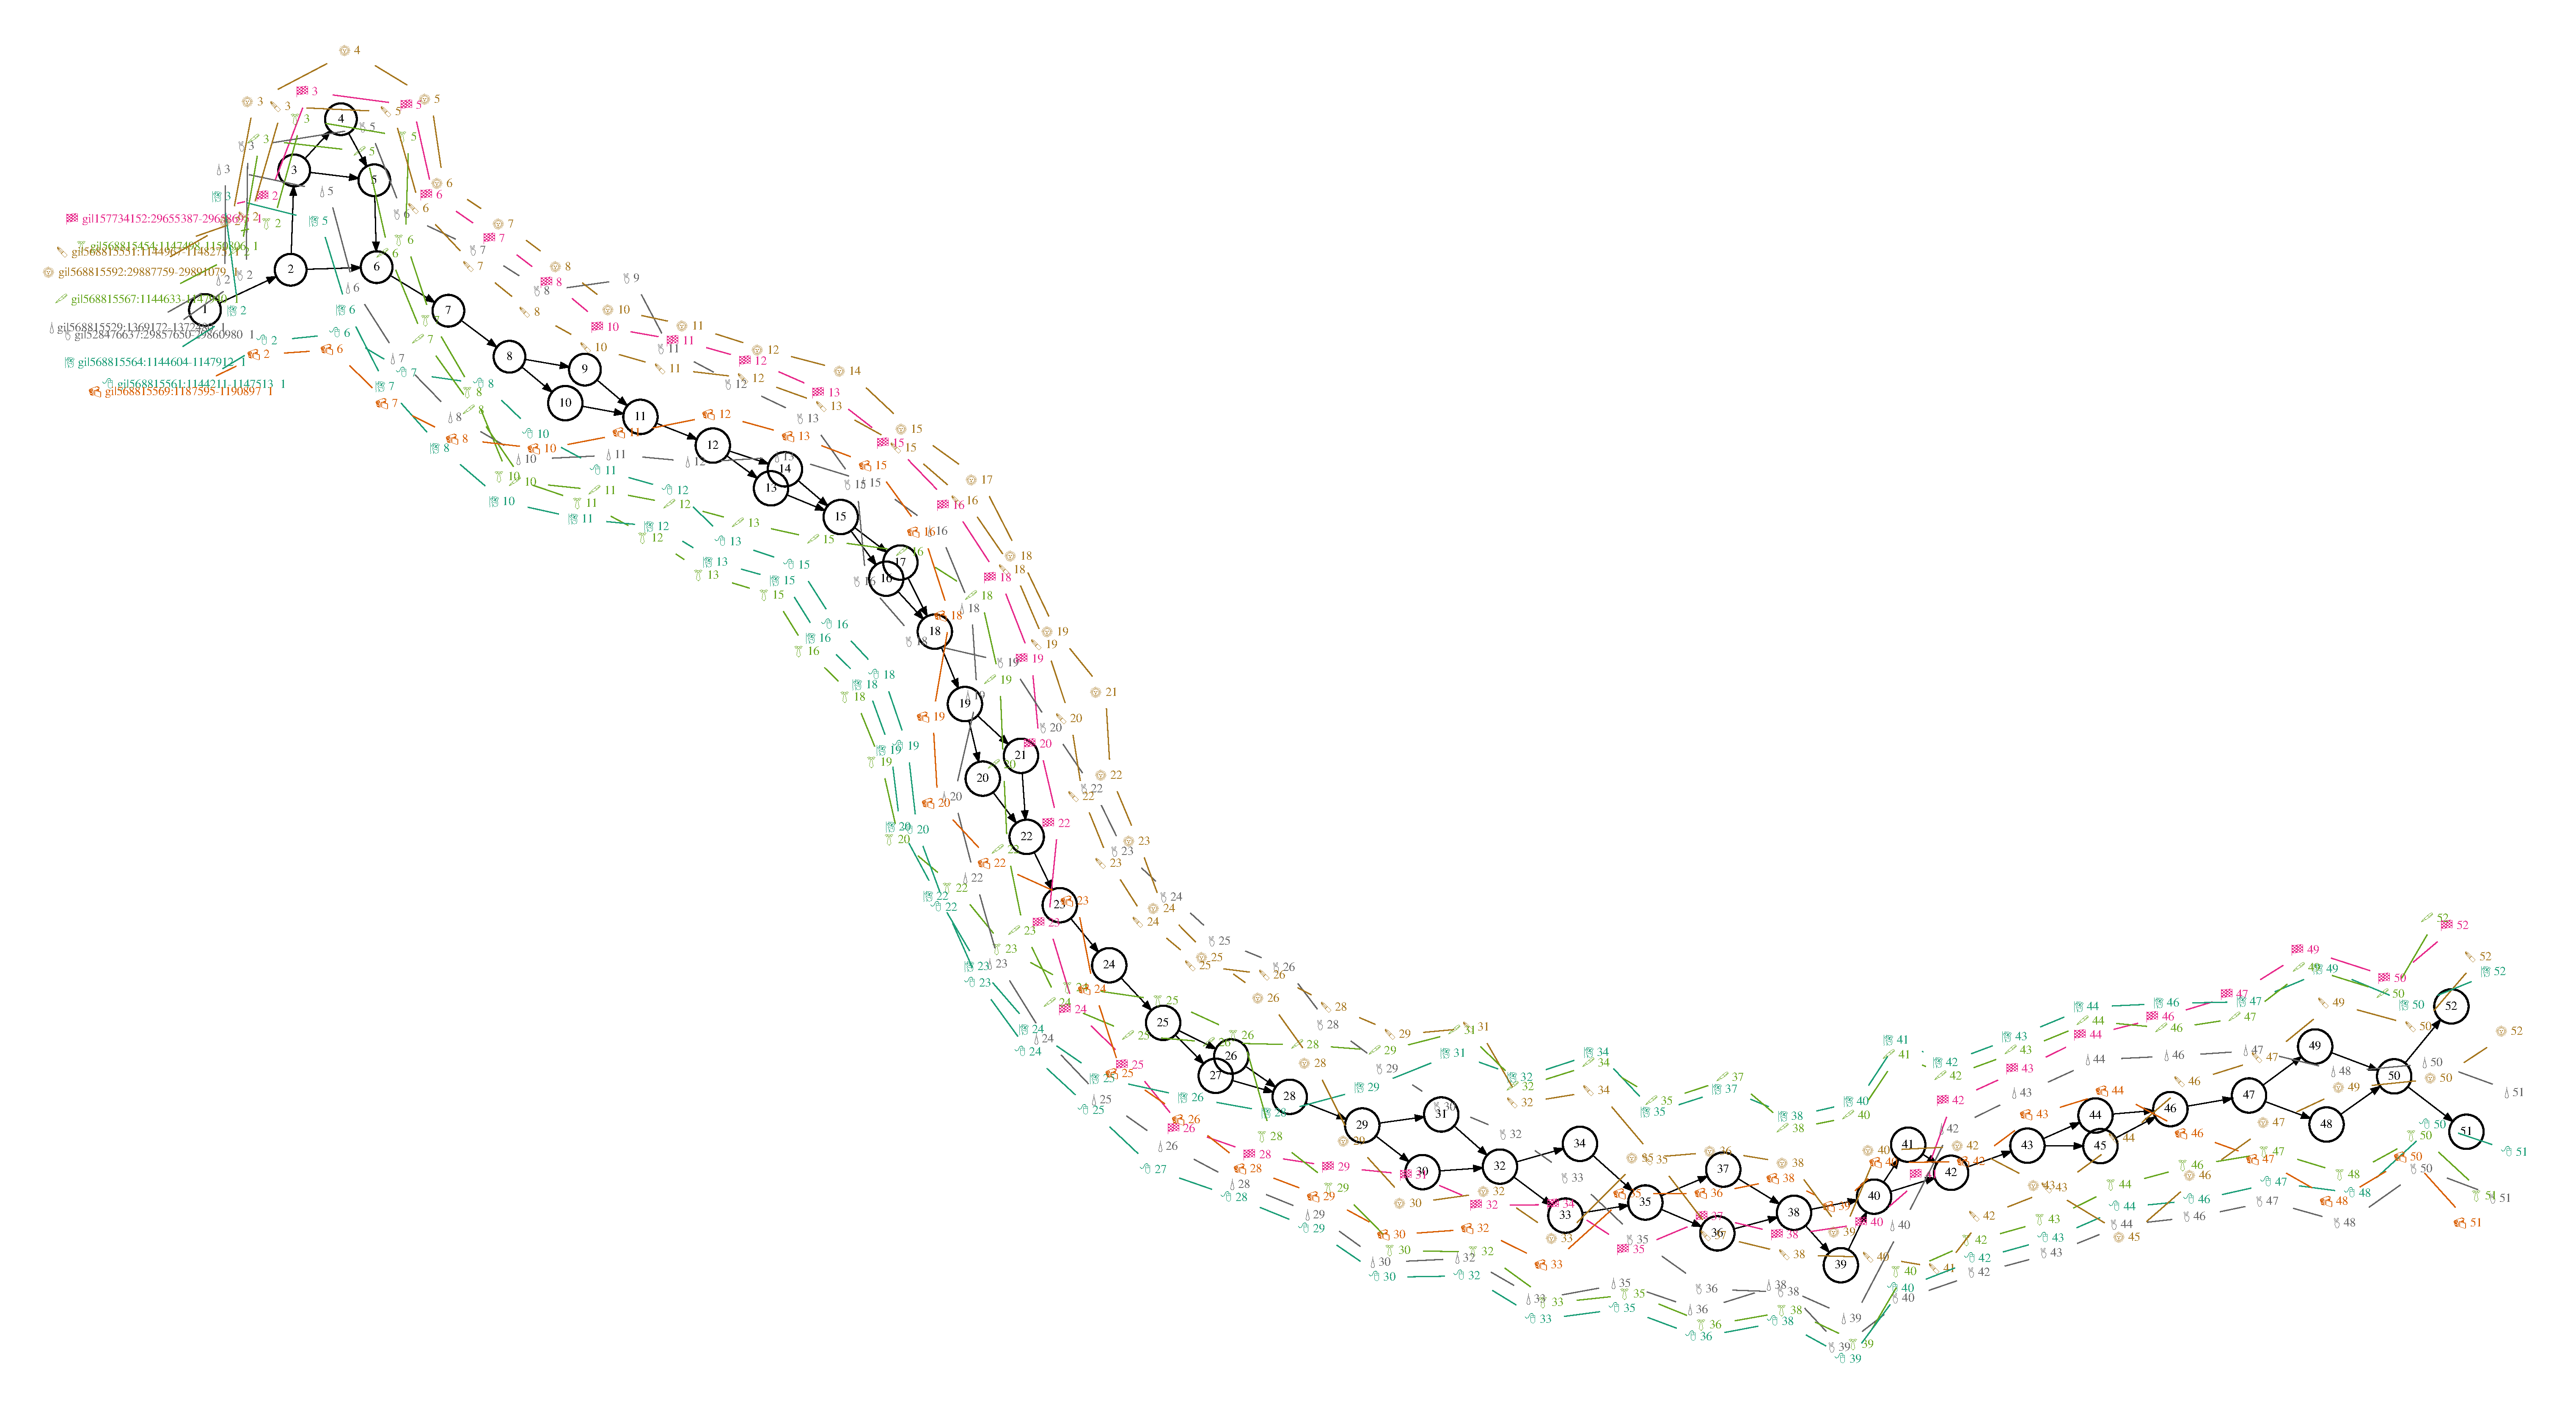
\includegraphics[width=1.0\textwidth]{Chapter2/Figs/vg_view_dpS_H-3136_neato.pdf}
\caption[Force-directed layout with Graphviz's {\tt neato}]{
  A larger region of the same variation graph in figure \ref{fig:vg_view_dot} rendered using {\tt neato.}
    Here, each path in the variation graph is represented by a colored path, with the node steps 
    As in \ref{fig:vg_view_dot}, paths in the graph are represented as colored paths connecting node ids and emoji.
    The same hash function is used to determine the color and emoji combination used to label each path.
    Each mapping in each path corresponds to one such node id / emoji label, and it is connected to the previous and subsequent steps by a line of the same color.
    A hidden edge connects each of these path steps to the node it corresponds to.
    This link causes the force directed layout algorithm to draw each path mapping node close to the node it refers to.
    Note that the graphviz data input here rendered by {\tt neato} is the same as that given to {\tt dot} in \ref{fig:vg_view_dot}.
}
\label{fig:vg_view_neato}
\end{figure}

While this rendering captures the path space of the graph even in arbitrary graphs, it cannot scale to graphs of significant size due to its approximately $O(|N|^3)$ scaling.
The largest graphs I have visualized using this method contain tens of kilobases of sequence.
{\tt Bandage} \cite{wick2015bandage} is an alternative method which is oriented towards visualizing assembly graphs.
It reads GFA as input and provides an interactive rendering of the graph topology.
This approach can render graphs of up to tens of megabases.
Figure \ref{fig:vg_view_bandage} shows the properties of this technique using the same region of H-3136.

\begin{figure}[htbp!] 
\centering    
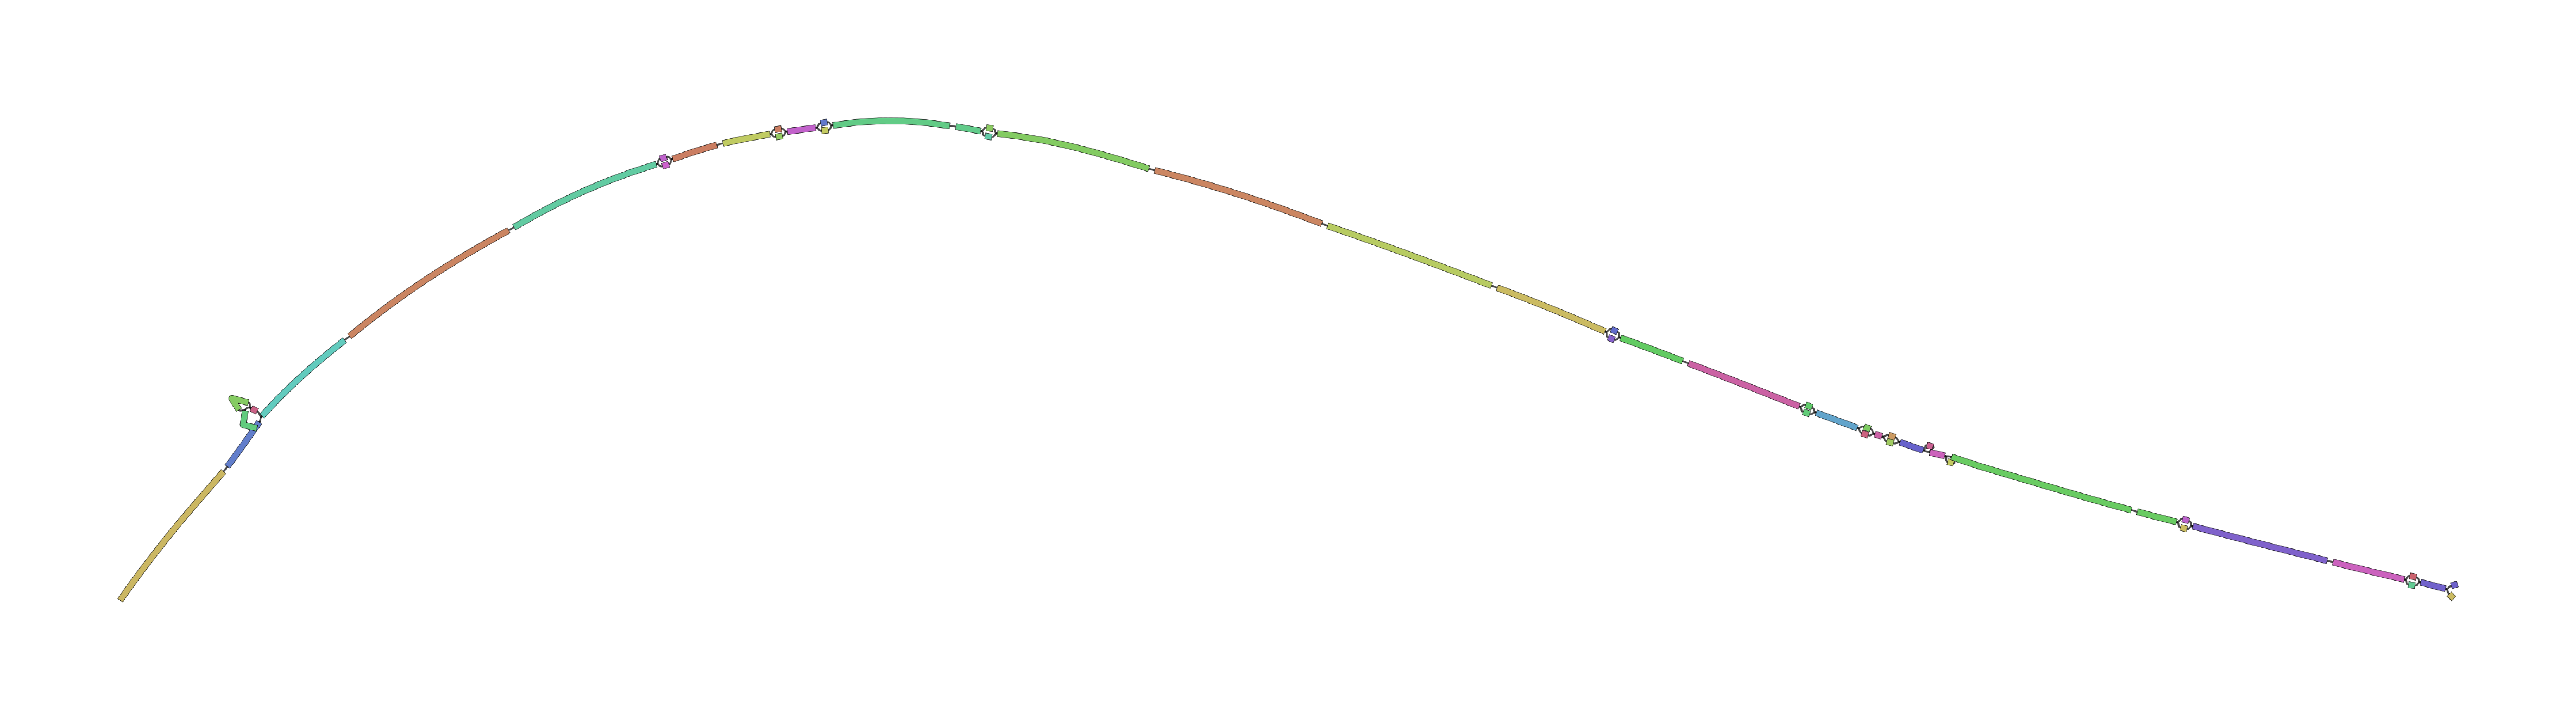
\includegraphics[width=1.0\textwidth]{Chapter2/Figs/vg_view_H-3136_Bandage.pdf}
\caption[Force-directed layout with Bandage]{
  The graph from figure \ref{fig:vg_view_neato} rendered using {\tt Bandage}.
  This rendering algorithm does not include the graph's paths.
  Here, node colors have been randomly assigned, and serve to indicate where nodes start and end.
}
\label{fig:vg_view_bandage}
\end{figure}

\subsection{Linear time visualization}

Graph layout algorithms are computationally complex due to their need to iteratively relate all components of the graph to all others.
In these layouts, we can observe large scale features about the topology and organization of the graph.
These views are helpful in many contexts, but the computational complexity of obtaining them prevents us from quickly visualizing larger graphs.
Also, they do not scale efficiently to large path sets, and it is often difficult to understand alignments or other path-related on the graph using them.

To resolve these issues I developed a linear time rendering algorithm that projects a given VG, as indexed by XG, into a vector graphics format using the widely-available graphics library {\tt libcairo}.
This visualization algorithm uses the sequence basis vector $S_\textbf{iv}$ as a coordinate system to position all elements of the graph.
The graph topology itself is laid out in accordance with the node representation in $S_\textbf{iv}$, flowing from left to right at the top of the rendering.
Node lengths are shown using a black bar, with the sequence labels given below.
The graph topology is rendered above the node set, and layout of these edges can be completed in linear time as they are rendered as simple splines connecting node ends.
Paths, or other annotations such as coverage per read set, are displayed below as colored bars matching the subset of the node space that they cover.
Where paths traverse a given node multiple times, an annotation is added to indicate the copy number.
This technique is implemented as {\tt vg viz}, and an example rendering is given in figure \ref{fig:vg_viz}.

\begin{figure}[htbp!] 
\centering    
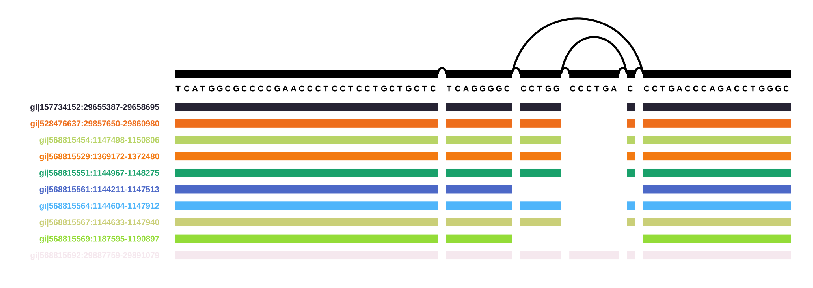
\includegraphics[width=1.0\textwidth]{Chapter2/Figs/vg_viz_H-3136.pdf}
\caption[Linearized variation graph visualization]{
  The same variation graph in figure \ref{fig:vg_view_dot} rendered using {\tt vg viz}.
  Above, we see the graph topology in terms of nodes, their lengths, and the edges that link their ends.
  Node sequence labels are shown below this topology, at the nodes they correspond to.
  Below, each path in the graph occupies a single position on the vertical axis.
  A hash function projects each path into a color, although the specific mapping is not the same as in figures \ref{fig:vg_view_dot} and \ref{fig:vg_view_neato}.
  Each horizontal position corresponds to a unique graph position.
  Where a path touches this graph position, we applied a colored bar at the given vertical axis position corresponding to the path.
  This rendering thus represents paths as binary vectors over the sorted sequence space of the graph.
}
\label{fig:vg_viz}
\end{figure}

It is important to recognize that this approach is lossy.
Path ordering is not clearly represented, as the paths are treated like masks over the sequence space of the graph.
Furthermore, it can be difficult to interpret complex graphs as the topology of the graph is obscured in the simplistic rendering.
{\tt vg viz}'s linear layout treats the graph sequences as a basis space in which other paths or alignments may be interpreted.
This simplistic view is central to many potential applications of {\tt vg}, which I further discuss in section \ref{sec:basis_space}.
The linear scaling of the algorithm should allow it to be applied to whole genomes, provided suitable front-end visualization software can be built, such as in a web interface.

\section{Graph mutating algorithms}

To use variation graphs as reference systems, we need to be able to modify them.
Algorithms in graph theory are frequently based on graph transformations, and I have discussed some of them in the context of assembly and whole genome alignment.
{\tt vg} implements many algorithms that alter the graph, but a number are of importance to its development as a system for resequencing, and I detail them here.

\subsection{Edit}

As discussed in section \ref{sec:extending}, the extension of a variation graph to include new sequences and paths can be thought of as a transformation yielding a bijection between the new and old graphs $edit(G, A) \to (G', \Phi)$.
The main issue which adds complexity to this process is that nodes represent more than a single character.

If nodes did represent a single character, then they would remain atomic through graph extension.
It is simple to edit a ``basepair'' graph of this type: $G = (N, E, P)$, where $\forall_{n \in N}{|seq(n)| = 1}$.
We walk through the alignments to it $A = a_1\ldots a_{|A|}$, adding novel bases represented in them ($seq(A) \notin G = N_A$) as new nodes.
Then for each alignment $a_i$, we add edges connecting nodes in the order they would be traversed by the path of the alignment embedded in the graph $p_{a_i} \in G'$, yielding $E_A$.
Finally, we add paths representing the embedded alignments $P_A$.
The resulting graph unifies these additions $G' = (N \cup N_A, E \cup E_A, P \cup P_A)$.

To achieve lower representation costs in graphs with sparse variation, we usually compress the graph so that nodes cover multiple bases and thus we must consider the editing process in multiple phases.
We first modify graph $G$ so that every novel sequence will be added at the start or end of a node.
We do this by breaking nodes into multiple derivative nodes when they overlap mappings that do not match the graph using $break(G, A) \to (G', \Phi)$.
For instance, if $seq(n_i) = {\tt GATTACA}$ and we have a SNP ${\tt T} \to {\tt C}$ at offset 4, we would obtain $n_i \to n_i', n_i'', n_i''' : seq(n_i') = {\tt GAT} $, $seq(n_i'') = {\tt T}$, $seq(n_i'') = {\tt ACA}$.
We can then apply $translate(A, \Phi) \to A'$, and add edges to $G'$ implied by the alignments as we would when editing a graph with single character nodes.

\subsection{Pruning}
%*2.5p 3h*

The number of paths in a sequence graph grows exponentially with the number of variable sites.
As I have discussed, this causes problems for alignment algorithms and graph sequence indexing.
While we can use efficient disk-backed index construction algorithms like GCSA2 to mitigate the effects of this exponential scaling, only a handful of dense clusters of variation in the graph can increase the memory requirements of path enumeration beyond any reasonable level.
To control this we restructure the graph to limit recombinations in the global sequence index.

We have explored two main techniques for the reduction of graph complexity.
In the first, we prune regions of the graph which have high path complexity using a depth-first search (DFS).
We can optionally add back known haplotypes, in order to mitigate the loss of information from the index.
For VCF-based VGs, where we have haplotype panels, the performance of local alignment is unaffected by the topological complexity, so we only need to apply this pruning to the graph input to GCSA2 indexing.
In assembly graphs, we find that nodes which represent repeats can sometimes have extremely high degree, which causes problems both for indexing and local alignment to the graph.
There, we must remove these nodes in order to use the graph even for local alignment.

\subsubsection{\emph{k}-mer \emph{m}-edge crossing complexity reduction}

In $k$-mer complexity reduction, we enumerate the $k$-mers of the graph, removing edges when a given $k$-mer crossing them would cross $> m$ edges.
We implement this filter, $prune(G, k, m) \to G_\textbf{simple}$, using the $k$-mer enumeration algorithm that generates a DBG from the variation graph, only that our walks through the graph are bounded at $m$ edge crossings.
For each offset in each node $n_i$ and $\overline{n_i}$, we run a DFS forward until we have read $k$ characters of the graph.
During the pruning operation, instead of emitting the $k$-mers with their contexts, we stop the DFS when we have crossed $m$ edges.
We record the edge in $E_\textbf{complex}$. % = \{ e_{ij} : \exists p \in G : |p| > m \mbox{, } node(p_{|p|-1} = i) \mbox{, } node(p_{|p|}) = j \}$.
We thus derive the subgraph from the current graph by removing the complexity-inducing edges: $(N, E \setminus E_\textbf{complex}, P) \to G_\textbf{simple}$.
It can be helpful to remove any small isolated components that result from this pruning, which can be done with a linear subgraph enumeration algorithm and the measurement of the sequence length of each.
A disjoint component $G_\textbf{sub} \in G_\textbf{simple} : \forall_{e_{ij} \in N_\textbf{sub}} n_i \in N_\textbf{sub} \land n_j \in N_\textbf{sub}$ must have length $\sum_{\forall n \in N_\textbf{sub}} |seq(n)| \geq {\cal J}$.
By default, we use $k=24$, $m=3$, and ${\cal J}=33$.

\subsubsection{Filling gaps with haplotypes}

Although removing complex regions will reduce the number of recombinant haplotypes represented by the graph, it is likely to also remove sections of known haplotypes.
We can retain the complexity reduction without losing sequences in known haplotypes by replacing the pruned regions in $G_\textbf{simple}$ with unfolded copies of each haplotype sequence.
When we have a single reference path in $G_\textbf{ref}$, we can accomplish this by overlaying $G_\textbf{simple}$ and $G_\textbf{ref}$.
However, this will not achieve the desired result with even two overlapping paths, as where these differ they would reintroduce the re-combinatorial explosion that we hope to resolve with pruning.
An alternative is to copy the haplotypes in the GBWT index that stretch from one border to the other of each removed region into the removed subgraphs in $G_\textbf{simple}$.
Doing so, we must preserve a mapping between the new nodes and the previous underlying ones in $G$.
This allows matches to the haplotypes to be converted into matches in the base graph.
The exact method by which this filling implemented is described in \cite{siren2018haplotype}.

\subsubsection{High degree filter}

Because they separate dense variation into heterozygous bubbles, assembly graphs may feature greater ``smoothness'' than VCF-based graphs locally.
But, in the context of repeats, they can contain nodes with exceptionally high degree.
If these cluster together then they generate highly-connected regions that introduce degeneracy in the path space of the graph, and cause problems for $k$-mer enumeration and GCSA2 indexing.
Furthermore, the local alignment methods in VG do not support efficient alignment through such dense regions.
Preventing this is relatively simple, in that we remove nodes with more than ${\cal D}$ edges linking them to the graph, yielding $G_\textbf{prune} : \forall_{n_i \in N_\textbf{prune}}{{\cal D} \geq |\{ e_{*i} \cup e_{i*} \cup e_{\overline{i}*} \cup e_{*\overline{i}} \}|}$.

It is not necessary that our local alignment suffers from high-degree nodes.
The problem is that GSSW is provided an alignable graph that is an extracted subset of the full graph.
If this subgraph is extracted using context expansion in the graph, then high-degree nodes will generate extremely large subgraphs.
One solution would be to use the bit-parallel string to graph alignment approach in \cite{rautiainen2018bit}, as this achieves optimal bounds in the size of transformed graph to which we align.
Alternatively, the graph exploration should be more directly linked to the alignment process.
The X-drop aligner {\tt dozeu} could be adapted to this approach, as the X-drop parameter would provide a natural limit to the graph exploration.
Such approaches may allow us to tolerate a larger ${\cal D}$, but it seems unlikely that they will allow alignment to be driven through the most-tangled areas of the graph without a large performance penalty relative to graphs with lower maximum degree.

\subsection{Graph sorting}
%*1p 1h*

To achieve as much partial ordering as possible, we order and orient the nodes in the graph using a topological sort.
The sort is guaranteed to be machine-independent given the initial graph's node and edge ordering.
The algorithm is well-defined on non-DAG graphs, but in these cases the order is necessarily not a topological order.
Our approach is a bidirected adaptation of Kahn's topological sort \cite{kahn1962topological}, which is extended to handle graph components with no heads or tails.
This algorithm can be understood as a kind of seeded depth first search through the graph.
Where the graph has nodes which are pure heads, it begins there.
Otherwise, a set of seed nodes which are stably selected given a particular graph are used to begin the sort.
The details of this procedure are provided in algorithm \ref{alg:pseudotoposort}.

Sorting can provide a simple optimization during read alignment.
If the reference graph has been sorted, then we can use the given order to generate node identifiers, embedding the rank of each node in its id.
We can detect if a given subgraph is possibly non-acyclic if $\exists e_{ij} \in E : i > j$, and if so submit the graph to sorting, unfolding, and DAGification before applying local alignment.

Similarly, the sort allows us to project data in the context of the graph into a single dimension.
Provided the graph is regionally partially ordered, this projection preserves local structures, which is a desirable property.
This makes the sort applicable to visualization techniques as in figure \ref{fig:vg_viz}.

\begin{algorithm}
  \caption[Pseudo-topological sort]{Pseudo-topological sort}
  \label{alg:pseudotoposort}
  \begin{algorithmic}
    \State $G = (N, E, P)$
    \Comment{A copy of our input graph which we will destructively modify}
    \State $L \gets [ \ldots ]$
    \Comment{Stores the pseudo-topological order}
    \State $S \gets \emptyset$
    \Comment{Set of nodes which have been oriented but not yet traversed}
    \State $V \gets \{ n_i \} \in N : \not \exists e_{ji} \forall n_j \in N$
    \Comment{We start from the head nodes of the graph}
    \If{$V = \emptyset$}
    \Comment{If there are no head nodes, we use ``seed'' nodes}
    \State $V \gets \text{Stably-selected seed nodes} \in N$
    \EndIf
    \While{$V \neq \emptyset$}
      \State $n \gets n \in V$
      \Comment{Select a seed node}
      \State $V \gets V \setminus \{n\}$
      \Comment{Remove it from the input node set $V$}
      \State $S \gets S \cup \{n\}$
      \Comment{Store it in our working set $S$}
      \While{$S \neq \emptyset$}
        \State $n_i \gets n_i \in S$
        \Comment{Remove an oriented node from $S$}
        \State $S \gets S \setminus \{n_i\}$
        \State $L \gets [L[1] \ldots L[|L|], n_i]$
        \Comment{Append it to our output order $L$}
        \For{$\forall n_j : e_{ij} \in E$}
          \State $E \gets E \setminus \{e_{ij}\}$
          \Comment{Remove the edge from our edge set}
          \If{$\not \exists e_{kj} \forall k \in N$}
          \Comment{$n_j$ has no other edges to that side}
          \If{$e_{i\overline{j}}$}
            \State $n_j \gets \overline{n_j}$
            \Comment{Orient $n_j$ so the side the edge comes to is first}
          \EndIf
          \State $N \gets N \setminus \{ n_j \}$
          \Comment{Remove $n_j$ from $N$}
          \State $S \gets S \cup \{ n_j \}$
          \Comment{Insert $n_j$ into $S$}
          \Else
          \Comment{This helps start at natural entry points to cycles}
            \State $V \gets V \cup \{ n_j \}$
            \Comment{Record $n_j$ as a place to start when $S$ is empty}
          \EndIf
        \EndFor
      \EndWhile
    \EndWhile \\
  \Return{$L$} \Comment{Return our pseudo-topologically sorted order and orientation}
\end{algorithmic}
\end{algorithm}
 

\subsection{Graph simplification}

Assembly algorithms often employ a \emph{bubble popping} phase, in which small bubbles, which are graph components connected to the rest of the graph through a single source and sink node, are replaced by linear components representing the most-likely path through the bubble given the read data.
In {\tt vg} we can carry out a similar operation based on the bubble decomposition of the graph.
Unlike assembly graph bubble popping, we must retain information about the embedded paths and annotations in the variation graph.
Simplification has a number of potential applications, for instance in reducing the complexity of visualizations of large variation graphs.

\section{Graphs as basis spaces for sequence data}
\label{sec:basis_space}

If we can construct a graph which embeds all the sequences of all genomes which we are interested in, we resolve the separation between reference sequence and variation that is present in standard resequencing.
This suggests that the intermediate steps in resequencing may be made redundant.
If variation is already available during alignment then there is no need for a variant detection phase.
However, if the graph does not include variation in our samples, then variant calling is required.
In {\tt vg} we have implemented several methods to do so.
Similarly, we have implemented coverage summaries of read sets that may be used directly in downstream analyses.

\subsection{Coverage maps}

Numerous population genetic analyses are based on matrix representations of a collection of genomes.
Such models can be used to infer population structure and phylogeny, as well as to associate phenotypes to genomic variants.
If the variation graph used as a reference contains all sequences relevant to our analysis, then a matrix of per-base coverage of the graph by sample will provide highly representative information to downstream analyses.
Exceptions include structural variation that does not result in coverage changes, such as balanced events like inversions.
Also, some local patterns of variation between successive small variation will not be distinguishable.
If we were to annotate edges with their coverage, this method would produce a result equivalent in information content to a Markov model.
It is thus clear that any coverage based index will be lossy relative to the full read set.
However, the lossiness reduces the information cost of storing and processing these coverage maps.
As I described in section \ref{sec:coverage_index}, in {\tt vg} I developed an efficient method to accumulate coverage information of this kind across the graph.

\subsection{Bubbles}

In a sequence graph, a \emph{bubble} is a pair of paths which start and end at the same nodes ($s$, $t$) but are otherwise disjoint in the graph \cite{zerbino2008velvet}.
Bubbles encompass our intuition about genetic variation in graphs.
A homologous sequence corresponding to the common start and end nodes in the bubble flanks two or more alternative alleles in the middle.
These structures were first considered in the context of finding small variation, and it was only in recent years that methods were developed to efficiently enumerate all bubbles of any size in DAGs \cite{birmele2012efficient}.

Bubbles can nest and contain more complicated internal structures between the paths through them.
The bubble may be generalized to the idea of a \emph{superbubble}, which is a directed, acyclic component of a graph with a single head and tail node \cite{onodera2013detecting}.
As for bubbles, efficient enumeration of superbubbles is possible in a DAG \cite{brankovic2016linear}.
The optimal method relies on a recursive topological sort of the graph to structure the nested bubbles.
Candidate node starts ($s$) and ends ($t$) are found following the definition of a superbubble.
The set of candidates is then validated by range min queries (RMQ) to produce the set of superbubbles.
As sort is linear $O(|N| + |E|)$, and the candidate enumeration and RMQ may be implemented on the sorted graph in $O(1)$ each, this yields a linear time algorithm for the enumeration of superbubbles.

The DAG requirement of this method is a significant limitation.
In order to apply the superbubble enumeration to an arbitrary graph we must first DAGify it.
In response, I worked with Benedict Paten and others to generalize the idea of a genetic site to support arbitrary bidirectional sequence graphs \cite{paten2018superbubbles}.
To formulate a generalization of superbubbles, we introduce the concept of a \emph{snarl}, which is any graph component connected to the rest of the graph by two or fewer bordering nodes\footnote{In the paper the formulation is based on a bi-edged graph akin to the Enredo graph, but we note that a node-based formulation is equivalent and matches the other models in this section.}.
Snarls whose internal separated component is acyclic and does not contain any tips are \emph{ultrabubbles}.

Paten observed that trees embedded in the Cactus graph transformation of a variation graph corresponded to the standard concept of superbubbles.
Specifically, the cactus graph is transformed into a \emph{cactus tree} in which each simple cycle in the cactus graph becomes a special kind of node.
Various rootings of this tree may then be used to define a hierarchy of bubbles.
The bidirectional nature of the variation graph mean that snarls can embed each other in a manner akin to how the twist used to generate an M\"{o}bius strip results in it having a single surface and border.
In these cases the resulting cactus tree will support multiple alternative ultrabubble tree rootings, and so unlike the bubble and superbubble decompositions for DAGs the ultrabubble decomposition is not unique.
We can enumerate a subset of these by identifying bridge edges (typically representing tips) in the ``bridge forest'', which is the result of a contraction of the cycles in the cactus graph into a set of top-level cycle representing nodes, and then use them to produce various rootings of the cactus tree.

Ultrabubbles and superbubbles provide a natural framework in which to reason about the hierarchy of variable genetic sites embedded in a graph.
As such they provide the basis for generic models of genotype inference based on variation graphs which are capable of genotyping any kind of genetic variation, including structural variation as well as nested variation, in the same model as SNPs and indels.

\subsection{Variant calling and genotyping}

Given a definition of variable genetic loci in the graph, we can build a genotyping system capable of generating genotype calls in the context of the graph.
In {\tt vg} we have explored two such methods.
The first, originally implemented in {\tt vg call}, generalizes the concepts first implemented in {\tt samtools mpileup} to work on the graph.
A set of alignments are first reduced to pointwise edits against the graph and per base coverage of the graph.
This graph ``pileup'' is then processed by a genotyping algorithm that considers genetic sites using the ultrabubble model.
A schematic overview of the method is shown in figure \ref{fig:vg_call}.

\begin{figure}[htbp!]
  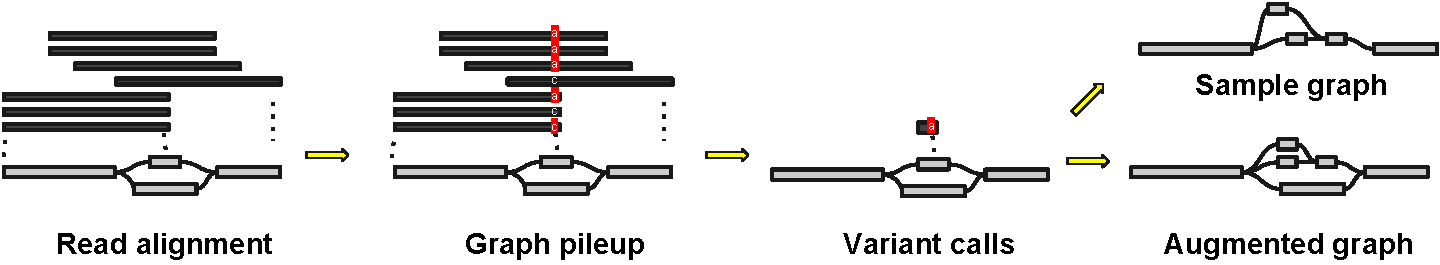
\includegraphics[width=1.0\textwidth]{Chapter2/Figs/vg_call.pdf}
  \caption{
    Pileup variant calling with {\tt vg call}
    }
  \label{fig:vg_call}
\end{figure}

The second model, implemented in {\tt vg genotype}, embeds the alignments in the variation graph using $edit(A, G_\textbf{base}) \to (G_\textbf{aug}, \Phi_{\textbf{aug}\to\textbf{base}})$, and then genotypes across the ultrabubbles of $G_\textbf{aug}$ which are supported by reference paths in $G_\textbf{base}$ or reads.
As the resulting genotypes are represented as unordered sets of paths in $G_\textbf{aug}$, they are projected back into the coordinate space of $G_\textbf{base}$ using the translation $\Phi_{\textbf{aug}\to\textbf{base}}$.
An overview of the process is shown in figure \ref{fig:vg_genotype}.

\begin{figure}[htbp!]
  \centering
  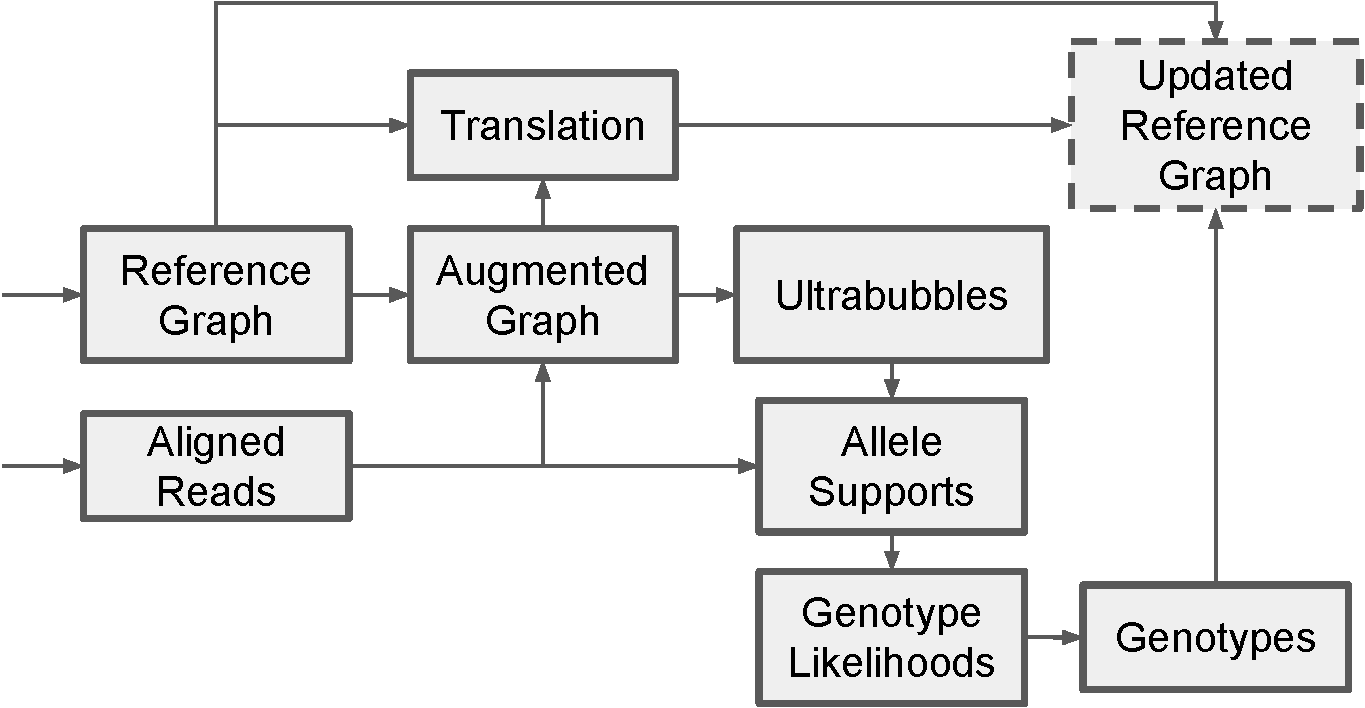
\includegraphics[width=0.7\textwidth]{Chapter2/Figs/vg_genotype.pdf}
  \caption{
    Graph augmentation-based variant calling in {\tt vg genotype}
    }
  \label{fig:vg_genotype}.
\end{figure}

While principled, the full augmentation model in {\tt vg genotype} is very expensive to compute.
The pileup model has proven to be more efficient.
Over time {\tt vg call} has been adjusted to implement some features of the full graph augmentation model in {\tt vg genotype} where the graph is augmented only with sequences supported by some number of alignments at a given quality threshold.
Both methods employ a diploid specification of the genotyping model in freebayes \cite{garrison2012haplotype} to develop their posterior estimates of variant quality.
The generalization of SNP and indel calling to haplotype calling implemented in freebayes corresponds to the same allele model used in both {\tt vg} variant calling methods.
Alleles correspond to DNA sequences of arbitrary length, anchored at the ends to the reference genome (in the case of freebayes) or to the rest of the graph (as in the ultrabubbles used in {\tt vg}).

The complexity of running and evaluating genotyping in the graph has slowed development of these methods.
Currently they are still outperformed by standard variant calling methods based on the linear reference, as indicated by our results in the PrecisionFDA variant calling challenge that I will describe in the next chapter.

%\subsection{MEM matching to the bidirectional GBWT}

%\section{Contributions to related computational methods}

% in this chapter I've described things that I've done
% as a consequence of being in this work, here are things that I helped other people to build
% list papers, give references

% gpBWT
% GCSA2
% ...
